\documentclass[12pt, a4paper]{report}

\usepackage[utf8]{inputenc}
\usepackage[ngerman]{babel}
\usepackage{hyperref}
\usepackage{a4wide}
\usepackage{times}
\usepackage{pdfpages}
\usepackage{tabularx}
\usepackage[section]{glossaries}
\usepackage{todonotes}
\usepackage{multicol}
\usepackage{listings}
\usepackage{etoolbox}
\usepackage{subcaption}
\usepackage{fancyhdr}

%graphics
\usepackage{wrapfig}
\usepackage{graphicx}
\usepackage{float}

\pagestyle{fancy}
\fancyhf{}
\renewcommand\headrulewidth{0pt}
\cfoot{\thepage\ of \pageref{LastPage}}

\makeglossaries
\setcounter{tocdepth}{1}
% Inhaltsverzeicnis wird nur bis \section erstellt


\date{\today}
\title{Studienarbeit Mobile Quiz}
\author{Andrea Hauser und David Windler}



\begin{document}
	
	\begin{titlepage}
	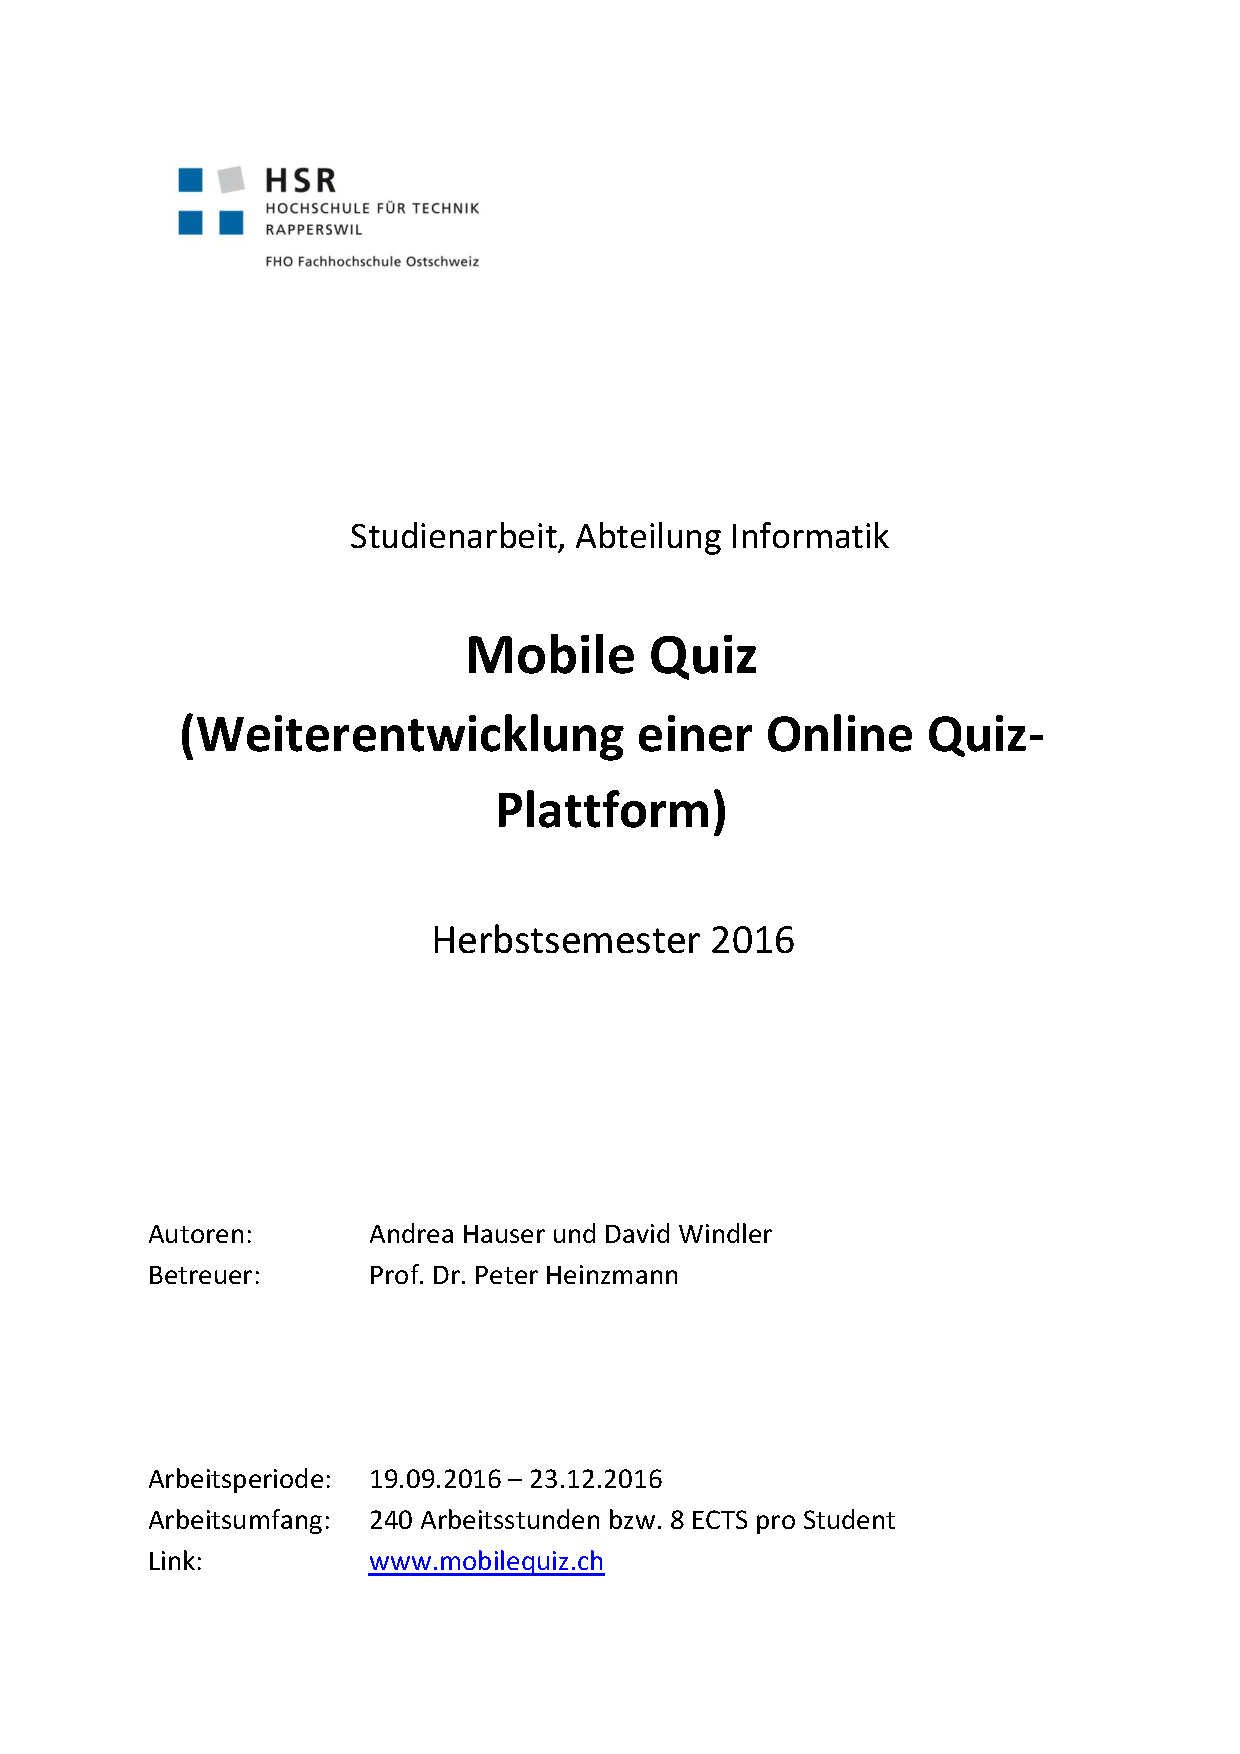
\includepdf{PDFs/Titelblatt}
	\end{titlepage}
	
	\noindent{\LARGE \textbf{Abstract}}
	
	\bigskip
	
	% !TEX root = Projektdokumentation.tex

%Die Kurzzusammenfassung (Abstract) richtet sich an Leute, die den Themenkreis der Arbeit relativ gut kennen. Für diese Leute beschreiben Sie die neuen, eigenen Resultate der Arbeit. Die Kurzzusammenfassung soll nur etwa 200 Worte (etwa 20 Zeilen) lang sein. Bei Studienarbeiten ist das von der HSR Schulleitung vorgegebene Kurzzusammenfassungsformular zu verwenden.

Mobile Quiz ist eine Online-Quiz Plattform für Computer und Smartphones, welche in verschiedenen HSR-Modulen (Computernetze, Informations- und Codierungstheorie, Informationssicherheit) und Weiterbildungskursen regelmässig eingesetzt wird. Mobile Quiz entstand 2012 aus einer Bachelorarbeit und wurde seither mehrmals erweitert. Die zu Beginn der Arbeit vorliegende Mobile Quiz Version umfasste zwar viele praktische Funktionen und Einstellungs-möglichkeiten, es mangelte aber an der Bedienbarkeit. Im Rahmen dieser Studienarbeit sollten einerseits die Benutzerfreundlichkeit erhöht und andererseits neue Funktionen hinzugefügt werden.

\bigskip

In einem ersten Schritt wurde Mobile Quiz gründlich untersucht. Mit einem Usability Test wurden Optimierungsmöglichkeiten für Quizteilnehmer bestimmt. Anhand der Behebung von kleinen Fehlern machte man sich mit dem Code und den eingesetzten Technologien vertraut. Diese umfassen PHP, HTML, CSS, Javascript, JQuery und Bootstrap. Im Rahmen einer Umfeldanalyse wurden ähnliche Online Quiz-Plattformen gesucht, getestet und bewertet. Die aus dieser Projektphase gewonnenen Erkenntnisse halfen bei der Neugestaltung der Seiteninhalte sowie bei der Festlegung von neuen Funktionen. Beim Design wurden die dargestellten Informationen bewusst auf das nötigste beschränkt. Zur Verbesserung der Benutzerführung wurden Symbole durch textuelle Menus ersetzt. Die Implementierung erfolgte während fünf Wochen. Abgeschlossen wurde die Arbeit mit einem Usability Test. 

\bigskip


Die Bedienbarkeit von Mobile Quiz wurde durch diese Studienarbeit sowohl für Quiz-Ersteller, als auch für Teilnehmer wesentlich verbessert. Die Schritt-für-Schritt Benutzerführung erleichtert die Erstellung von Quiz, Fragen und Durchführungen. Dank der neuen Excel-Import Funktion lassen sich Quiz und Fragen einfacher erstellen. Durch die Erweiterung «Fragen mit Bildern» sind attraktivere Fragestellungen möglich. Die Konzeptänderung, welche pro Quiz mehrere Durchführungen möglich macht, erleichtert den Einsatz von Mobile Quiz im Unterricht mit mehreren Übungsgruppen. Dank dem neuen Design sollten sich die Quizteilnehmer schneller zurechtzufinden. Dies belegt der Vergleich der Ergebnisse der beiden Usability-Tests vor und nach der Überarbeitung des Mobile Quiz.  
Die jetzt vorliegende Mobile Quiz – Version wird ab dem nächsten Semester produktiv eingesetzt. Die Umsetzung der in der Analysephase ausgearbeiteten statistischen Auswertungen könnte im Rahmen einer weiteren Studienarbeit erfolgen. 
	\newpage
	
	
	\noindent{\LARGE \textbf{Aufgabenstellung}}
	\bigskip
	%Die unterschriebene Aufgabenstellung des Dozenten.
	% !TEX root = Projektdokumentation.tex


{\renewcommand{\arraystretch}{1.5}
\begin{tabular}{l l}
	Studiengang: & Informatik (I) \\ 
	\hline
	Institut: & ITA: Internet-Techn. und Anwendungen \\ 
	Gruppe: & Andrea Hauser und David Windler \\ 
	\hline 
	Betreuer: & Prof. Dr. Peter Heinzmann (Dozent) und Patrick Eichler (Assistent)
\end{tabular} 
}


\section{Ausgangslage}

In den Modulen Computernetze und Informationssicherheit können die Studierenden nach jeder Vorlesung ihr Wissen zum Vorlesungsstoff mit Hilfe der Webanwendung \url{www.mobilequiz.ch}  überprüfen. Die Studenten A. Hauser und D. Windler haben im Rahmen ihres Software Engineering Projekts ein Lernprogramm zum Thema AES Galois/Counter Mode erstellt. Sie wollten daher ihre Studienarbeit zum Thema Lernkontrollen durchführen.

Die MobileQuiz Lernkontrollen Anwendung wurde in den letzten Jahren im Rahmen von verschiedenen Studienarbeit entwickelt und erweitert. Seit der Überarbeitung durch HSR Assistent P. Eichler funktioniert \url{www.mobilequiz.ch} so stabil, dass es sogar in Prüfungen eingesetzt werden kann.  Dennoch gibt es Verbesserungs- und Erweiterungsmöglichkeiten, welche im Rahmen einer Studienarbeit bearbeitet werden können.

\section{Ziel}
Bei der bestehenden Anwendung \url{www.mobilequiz.ch} zur Durchführung von Lernkontrollen sollen weitere Fragetypen unterstützt werden. Es sollen ausführliche statistische Auswertungen zur Qualität von Fragen und Antworten möglich sein. Ferner soll mit einer generellen Überarbeitung die Bedienfreundlichkeit verbessert werden.

\section{Aufgaben}

\begin{enumerate}
	\item Einarbeitung, Analyse
	\begin{itemize}
		  \item Evaluation verschiedener Systeme zur Durchführung von Lernkontrollen (Vergleichstabelle)
		  \item Detaillierte Analyse der existierenden Anwendung \url{www.mobilequiz.ch} zur Durchführung von Lernkontrollen 
		  \item Durchführung von Usability Tests
		  \item Studium verschiedener theoretischer Untersuchungen zur computerbasierten Durchführung von Lernkontrollen (Abklärung und Übersicht zu Fragetypen)
		  \item Inbetriebnahme von Entwicklungs- und Dokumentationswerkzeugen
	\end{itemize}

	\item Refactoring
	\begin{itemize}
		  \item Inbetriebnahme von \url{www.mobilequiz.ch} auf HSR-Plattformen
		  \item Optimierung der aktuell vorhandenen Funktionen, Behebung von Fehlern (Offline Fragenerstellung und Excel Import/Export von Lernkontrollen, PDF Outputs, Sicherheitsprobleme)
	\end{itemize}

	\item Realisierung neuer Funktionen
	\begin{itemize}
		  \item Vereinfachung und Optimierung des Registrationsprozesses (Interessensgebiete, verbesserte Benutzerführung, Benachrichtigungen über neue Lernkontrollen), Erweiterung zur speziellen Behandlung von Benutzergruppen (Vorlesungsteilnehmende, Praktikumsgruppen)
		  \item Entwicklung neuer Fragetypen (Fragen mit Bildern)
		  \item Entwicklung neuer Antwortmöglichkeiten (Drag\&Drop)
		  \item Erweiterte statistische Auswertungen zu Fragen, Antworten und Resultaten der Teilnehmenden (Antwortzeit, Qualitätsmass für Fragen, Punktevergabe, Qualitätsmass für Antworten) 
		  \item Erweiterte Durchführungskontrolle (Zeitabstand von Wiederholungen bei mehrfachen Durchführungen)
	\end{itemize}
	
	\item Anpassungen für spezielle Use Cases
	\begin{itemize}
		\item Durchführung von Prüfungen
		\item Durchführung von Umfragen (Polls)
	\end{itemize}

	\item Dokumentation und Präsentation der Ergebnisse
  
\end{enumerate}

\section{Referenzen}
\begin{enumerate}
	  \item Hinweise zur Durchführung von Studienarbeiten: \url{https://dl.dropboxusercontent.com/u/4679041/SABA-Web-Anleitungen\_Heinzmann.zip}
	  \item Aktuelle Anwendung \url{www.mobilquiz.ch}  
	  \item Manuela Grob, Quiz, HSR Bachelorarbeit, HS2010.
	  \item Patrik Naef, Khalid Abdul, «Mobile Quiz», HSR Bachelorarbeit, 16.9.2012.
\end{enumerate}

\bigskip \bigskip
\parbox{6cm}{Rapperswil, \hrule
\strut \footnotesize Ort, Datum} \hfill
\parbox{5cm}{\hrule
\strut \footnotesize Betreuer}

	\newpage
	
	
	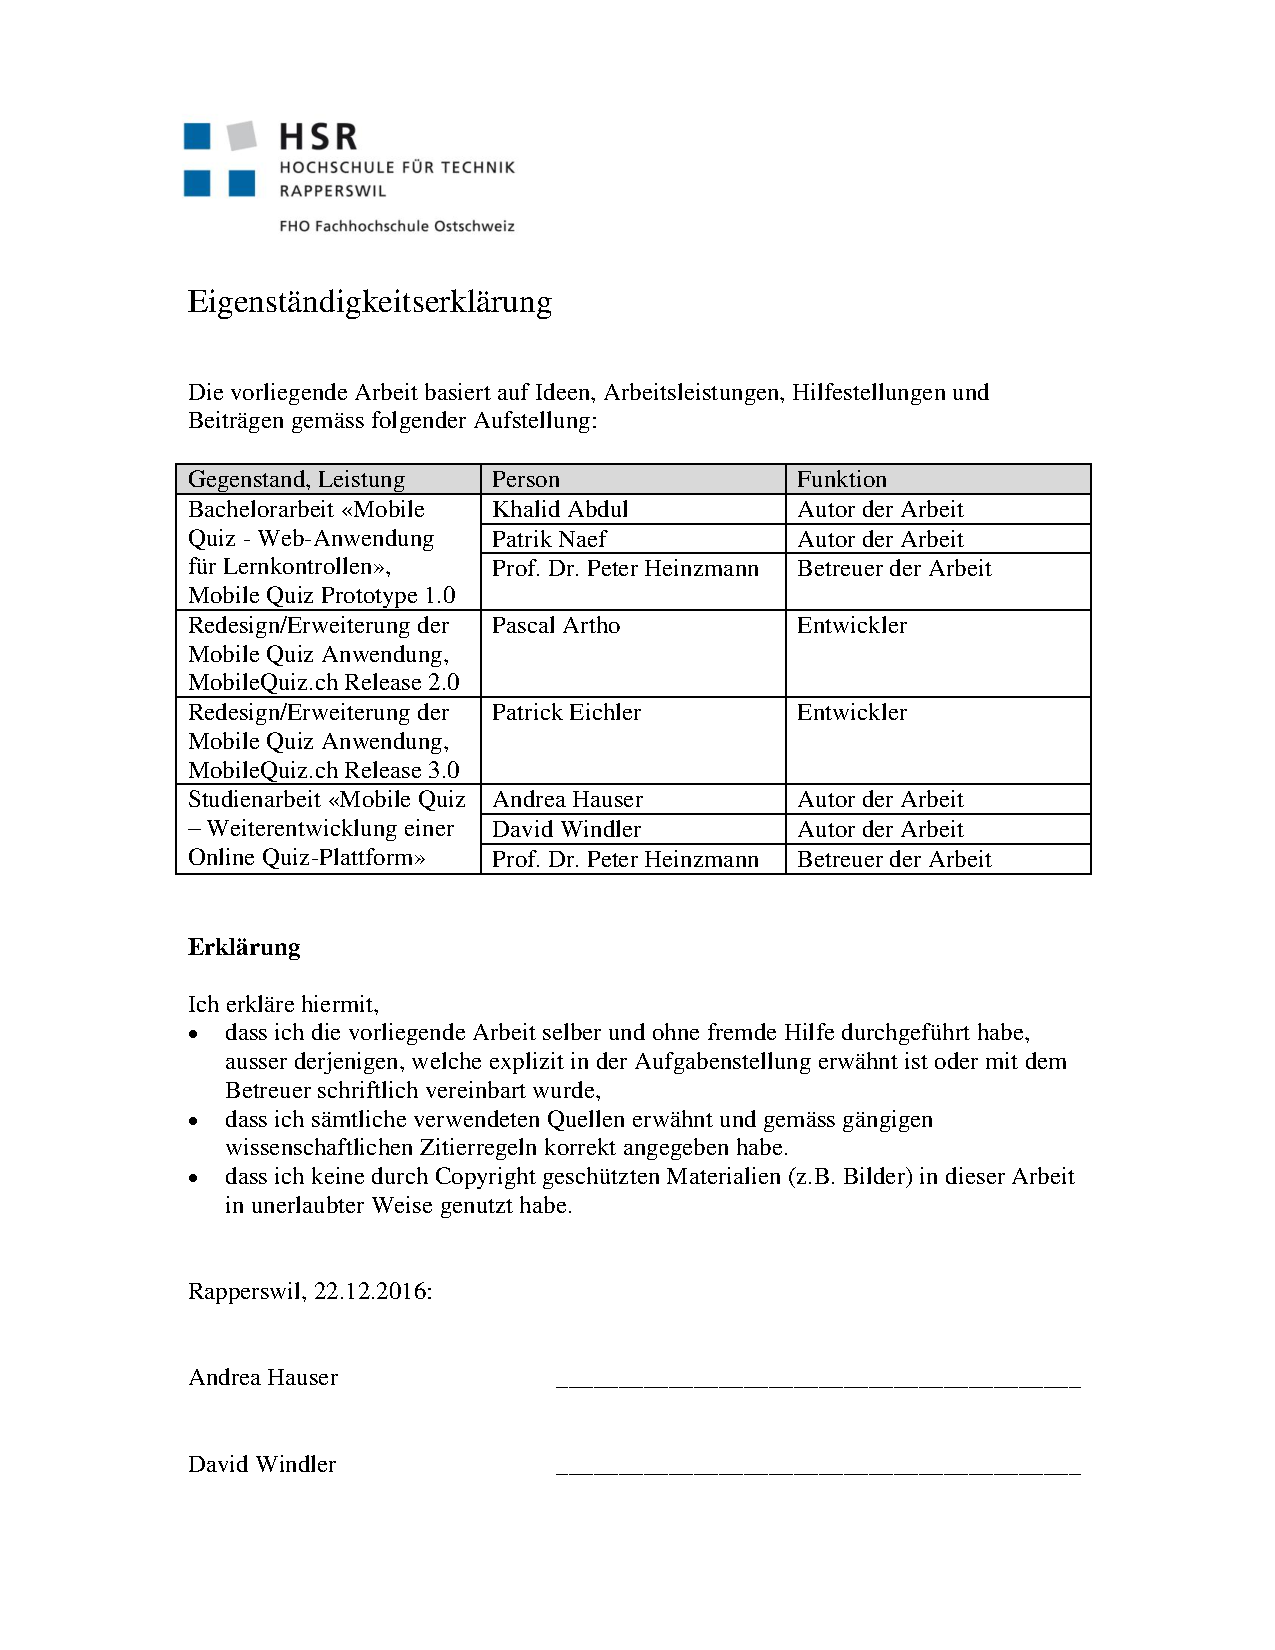
\includepdf[pagecommand={}]{PDFs/Eigenstaendigkeitserklaerung.pdf}
	%Unterschriebenes Formular "Erklärung zur Urheberschaft" Handelt es sich um eine Fortsetzung einer Studienarbeit, so ist in der HSR_Erklaerung_Urheberschaft klar aufzuzeigen, was im Rahmen der Studienarbeit und was bei der Bachelorarbeit gemacht wurde. In diesem Formular ist auch anzugeben, welche Informationen Copyright geschützt sind und daher nicht ohne Weiteres weitergegeben werden können.
	\newpage
	
	
	
\includepdf[pagecommand={}]{PDFs/Vereinbarungen_ueber_Urheber-und_Nutzungsrechte.pdf}
	%Unterschriebenes Formular "Vereinbarung zur Verwendung und Weiterentwicklung der Arbeit".
	\newpage
	
	
	\noindent{\LARGE \textbf{Management Summary}}
	
	\bigskip
	
	% !TEX root = Projektdokumentation.tex

Mobile Quiz ist eine Online Plattform, um Quizzes zu erstellen und zu lösen. Der Zugriff erfolgt via Computer oder Smartphone über einen Web-Browser. Die Plattform wird in verschiedenen HSR-Modulen (Computernetze, Informations- und Codierungstheorie, Informationssicherheit) und Weiterbildungskursen regelmässig eingesetzt. Die erste Version entstand 2012 aus einer Bachelorarbeit und wurde seither mehrmals erweitert. 

\bigskip

Vor allem Dozenten nutzen Mobile Quiz, um für Ihre Studenten Quizzes in Form von Lernhilfen während des Semesters zu bieten. Es besteht weiter die Möglichkeit die Quizzes entweder mit dem Typ Testatbedingung oder als Typ Prüfung zu erstellen und durchzuspielen. Die Wichtigsten Interaktionen mit dem Mobile Quiz System zeigt die folgende Abbildung.

\begin{figure}[H]
	\centering
	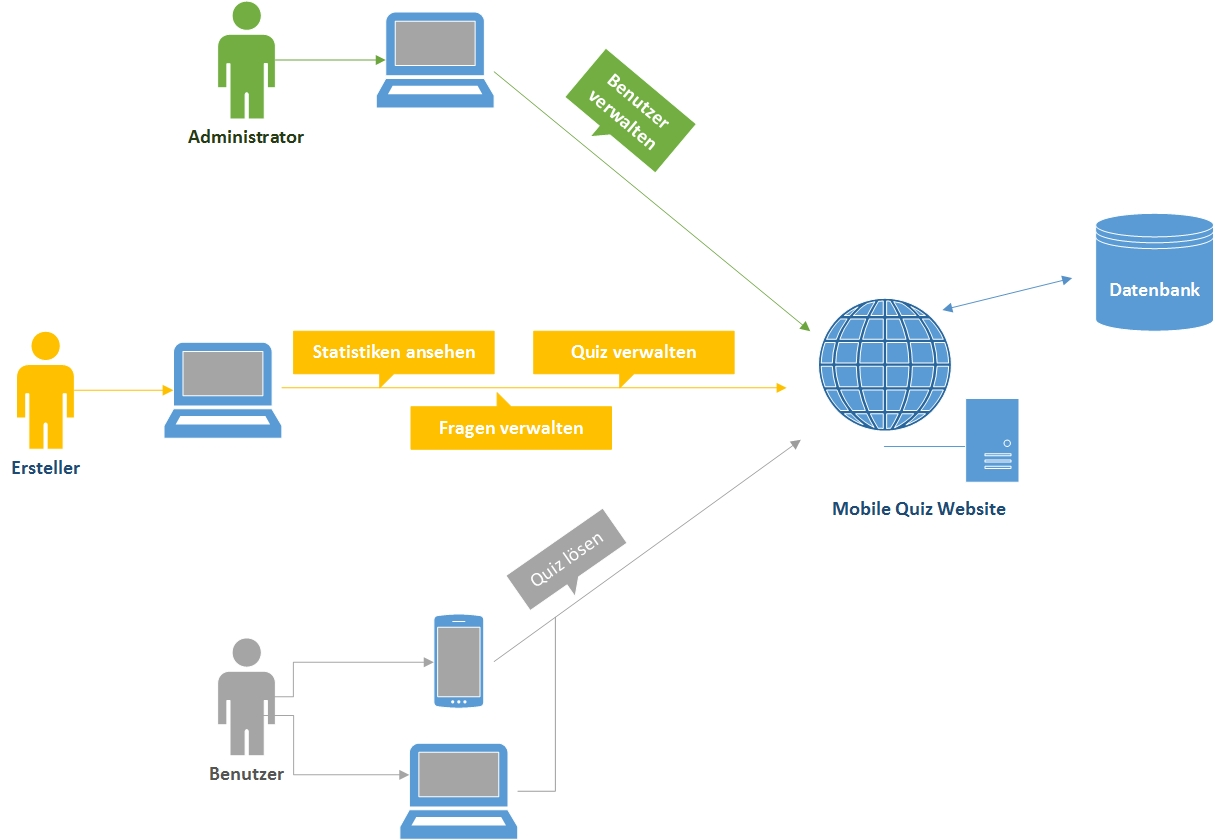
\includegraphics[width=1\textwidth]
	{Images/InteraktionMobileQuiz.jpg}
	\caption{Übersicht der wichtigsten Funktionen des Mobile Quiz}
\end{figure}

\bigskip
Die zu Beginn der Arbeit vorliegende Version umfasste zwar viele praktische Funktionen und Einstellungsmöglichkeiten, es mangelte aber an der Bedienbarkeit. Im Rahmen dieser Studienarbeit sollten deshalb einerseits die Benutzerfreundlichkeit erhöht und andererseits neue Funktionen hinzugefügt werden.

\bigskip

Das Vorgehen um sich in das Thema einzuarbeiten wurde wie folgt gewählt. In einem ersten Schritt wurde Mobile Quiz gründlich untersucht. Mit einem \gls{Usability-Test} wurden danach Optimierungsmöglichkeiten für Quizteilnehmer bestimmt. Durch die Behebung von gefunden Fehlern aus der eigenen Untersuchung machte man sich mit dem Code und den eingesetzten Technologien vertraut. Im Rahmen einer Umfeldanalyse wurden ähnliche Online-Quiz Plattformen gesucht, getestet und bewertet. Die aus den vorangegangenen Projektphasen gewonnenen Erkenntnisse halfen bei der Neugestaltung der Seiteninhalte sowie bei der Festlegung von neuen Funktionen. Beim Entwurf des Design wurden die anzuzeigenden Informationen bewusst auf das Nötigste beschränkt. Die Implementierung der Desings und Konzepte erfolgte während fünf Wochen. Da es sich bei dieser Arbeit um eine Erweiterung eines bestehenden Systems handelt, wurden die Technologien nicht neu gewählt. Es wurde die bereits bestehende Lösung mit PHP, JavaScript und JQuery für die Logik, der MySQL Datenbank für das Speichern der Daten und HTML zusammen mit CSS für die Darstellung verwendet. Nach der Implementierungsphase wurde die Arbeit mit einem zweiten \gls{Usability-Test} abgeschlossen.

\bigskip

Als Ergebnis dieser Arbeit konnte eine sowohl für den Quiz-Ersteller wie auch für den Teilnehmer wesentlich verbesserte Bedienbarkeit erreicht werden. Die Schritt-für-Schritt Benutzerführung erleichtert das Erstellen von Quizzes, Fragen und Durchführungen. Dank der überarbeiteten Excel-Vorlage können Fragen auch unterwegs, ohne eine Verbindung zum Internet, leicht erfasst und später hochgeladen werden. Durch die Erweiterung \glqq Fragen mit Bildern\grqq sind attraktivere Fragestellungen möglich. Die Konzeptänderung, welche pro Quiz mehrere Durchführungen möglich macht, erleichtert den Einsatz von Mobile Quiz im Unterricht mit mehreren Übungsgruppen. 

Mit Hilfe neuen Design sollten sich die Quizteilnehmer zudem schneller zurechtfinden. Dies belegt der Vergleich der Ergebnisse der beiden \gls{Usability-Test}s vor und nach der Überarbeitung der Online Plattform. 

\bigskip

Die jetzt vorliegende Mobile Quiz Version wird ab dem nächsten Semester produktiv eingesetzt. Die Umsetzung der in der Analysephase ausgearbeiteten statistischen Auswertungen sowie weiteren Konzepten könnte im Rahmen einer weiteren Studienarbeit erfolgen.
	%Das "Management Summary" bzw. die Zusammenfassung richtet sich in der Praxis an die "Chefs des Chefs", d.h. an die Vorgesetzten des Auftraggebers (diese sind weniger tief in die Thematik involviert als die direkt Beteiligten). Das Management Summary soll maximal 4 Seiten umfassen und mindestens eine Figur enthalten. Die Sprache soll knapp und klar sein.
	
	%Im Management Summary braucht es keine Untertitel. Die jetzt erstellten Titel sind eher als Vorgabe für den Ablauf gedacht.
	
	
	%Ausgangslage
	%	·         Ausgangslage (Warum wurde das Projekt durchgeführt? Was machen andere und welche ähnlichen Arbeiten gibt es zum Thema? Welche Ziele wurden gesteckt (Muss-, Soll-, Nice-to-Have Ziele)
	
	
	%Vorgehen
	%   ·         Vorgehen (Was wurde gemacht? In welchen Teilschritten? Wer war involviert (Durchführung, Entscheide, Zwischenprüfungen/Feedbacks usw.)? Verwendete Werkzeuge)
	
	
	%Ergebnisse
	%   ·         Ergebnisse (Was ist das Resultat des Projekts (quantifizierbarer und qualitativer Nutzen)? Was musste man selbst tun, was konnte von anderen verwendet werden? Selbstbeurteilung der  Zielerreichung in Bezug auf die Zielsetzungen der Arbeit. Abweichungen von den Zielsetzungen und Begründung dafür (positiv und negativ). Kosten. Lernpunkte aus der Durchführung des Projekts)
	
	
	%Ausblick
	%   ·         Ausblick (Verbleibende Probleme, Risiken und Gegenmassnahmen, was würde man anders machen? Wie geht es mit dem Projekt weiter, wer nutzt was? Welche weiteren Schritte, Entwicklungen, Anpassungen etc. werden empfohlen / sind geplant?)
	
		
	
	\tableofcontents
	%Im Inhaltsverzeichnis sollen Sie nur die Stufen Kapitel (h.), Unterkapitel (h.i) bzw. im Anhang die Haupt- (X) und Unterabschnitte (X.n) aufführen.
	\newpage
	
	
	
	\part{Hauptbericht}
	
	\chapter{Einleitung}
	% !TEX root = Projektdokumentation.tex

% 	Die Einleitung soll allgemein verständlich sein, d.h. sie soll beispielsweise auch für Ihre Freunde und Verwandten verständlich sein. Sie stellt die Aufgabe in einen grösseren Zusammenhang und liefert eine genaue Beschreibung der Ausgangslage und Problemstellung. Allfällige Vorarbeiten oder ähnlich gelagerte Arbeiten sind diskutiert. Zum Schluss der Einleitung können Sie auch beschreiben, welche Abschnitte des Berichts sich an welche Leser wenden (z.B. Anwender des Produkts, Entwickler, Betreiber).

%Überprüfen von Wissen \\
Während dem Studium werden viele Inhalte vermittelt und anschliessend mit einer Schlussprüfung abgeholt. Wie merkt ein Student aber schon vor der Prüfung, ob sein Wissen sattelfest ist? Mobile Quiz bietet eine Lösung dafür. Der Dozent erfasst Fragen, mit welchen die Studenten anschliessend ihren Wissensstand ermitteln können. \\
%Stand Mobile Quiz \\
Stand heute umfasst Mobile Quiz inzwischen einige Funktionen, um Quizzes zu erstellen. Verbesserungspotentiale liegen allerdings noch in den Bereichen der Bedienbarkeit, im Bereich von neuen Fragetypen sowie in der Auswertung von Quizzes. Durch letzteres wäre es dem Dozenten ersichtlich, welche Teile des Stoffs gut verstanden wurden und bei welchen noch Nachholbedarf herrscht. Somit könnte die Vorlesungszeit effizienter genutzt werden.
\\
%In dieser Arbeit wird XY umgesetzt.
\\
%Übersicht Kapitel \\
	
	%Die nach der Einleitung folgenden Hauptabschnitte richten sich in der Regel an die Nutzer und Betreiber des realisierten Systems und an die im entsprechenden Fachgebiet tätigen Ingenieure. Die Hauptabschnitte bilden typischerweise die wichtigsten Ergebnisse Ihrer Arbeit ab. Sie beschreiben das realisierte System bzw. die getätigten Untersuchungen. Die Leser sollen die zur Problemlösung getätigten Überlegungen verstehen. Theoretische Grundlagen sind soweit aufzuführen, als dies für die Lösung der Aufgabe nötig ist (keine Lehrbücher oder Wikipedia-Artikel (ab)schreiben). Die Erkenntnisse aus den theoretischen Untersuchungen sind also wenn immer möglich direkt mit der Problemlösung zu verknüpfen (z.B. mit eigenen Messungen oder mit Beispielen aus der schliesslich erstellten Anwendung zu illustrieren).
	
	%Sparen Sie nicht mit Diagrammen und Figuren. Diese müssen auch im Text diskutiert sein, d.h. es wird auch in Worten beschrieben, was man mit dem Diagramm oder der Figur zeigen will. Spezielle Details, welche die Kontinuität in den Hauptabschnitten stören, sind im Anhang aufzuführen.
	
	%Der Umfang der einzelnen Abschnitte des Berichts entspricht in der Regel dem Arbeitsaufwand, welcher für die entsprechenden Themen eingesetzt wurde.
	
	%Je nach Aufgabenstellung können beispielsweise Hauptabschnitte der folgenden Art vorkommen:
	
	\chapter{Bestehendes Produkt / Inbetriebnahme?}
	% !TEX root = Projektdokumentation.tex

\newglossaryentry{responsives CSS}{name={responsives CSS},description={CSS, welches die Seiteninhalte auf allen Bildschirmgrössen gut aussehen lässt.}}

\newglossaryentry{TLS}{name={TLS},description={Transport Layer Security ist ein Protokoll zur Sicherung der Kommunikation zwischen Client und Server.}}


\section{Eingesetzte Technologien und Werkzeuge}
MobileQuiz in der Version 3 verwendete die folgenden Technologien:

\begin{itemize}
	\item Apache2 als Web-Server
	\item PHP 5.6 als Server-seitige Programmiersprache
	\item MySQL als Datenbank
	\item HTML, CSS, JavaScript für den Seitenaufbau und die Interaktion
	\item jQuery für kürzere JavaScript-Befehle
	\item Bootstrap für \gls{responsives CSS}
\end{itemize}

Diese Technologiepalette wurde im Verlauf dieser Arbeit beibehalten und nicht erweitert. Die verwendeten Werkzeuge zur Entwicklung mit diesen Technologien sowie die restlichen, während dieser Arbeit eingesetzten Werkzeuge, sind im Anhang unter Kapitel \ref{chap:werkzeuge} aufgeführt. Beschrieben sind unter anderem der Einsatzzweck und der Bezugsort. Ergänzt wurden nützliche Hinweise, welche durch die Benutzung dieser Werkzeuge in Erfahrung gebracht wurden.


\section{Inbetriebnahme}
Das Aufsetzen der bestehenden Seite auf einer Server-Instanz der HSR dauerte länger als ursprünglich vorgesehen. Zu Beginn wurde das Aufsetzen mit Docker versucht, da die Server für die Studierenden neu damit ausgeliefert wurden. Anschliessend wurde eine neue Instanz mit reinem Linux Ubuntu bestellt, um die Seite ohne Docker in Betrieb zu nehmen. Beide Varianten scheiterten schlussendlich an der sicheren \gls{TLS}-Verbindung, wodurch diese dann im Code auskommentiert wurde.

Um ein weiteres Aufsetzen zu Erleichtern wurden zu beiden Varianten Anleitungen erstellt. Diese sind im Anhang unter \glqq V2 Apache\_PHP\_MySQL-Docker.tex\grqq und \glqq V3 Apache\_PHP\_MySQL-Ubuntu.tex \grqq zu finden.
Unter \glqq Anleitung Redmine Datenbank Backup\grqq ist dort ebenfalls das Einrichten eines täglichen Backups für die Sicherung der MySQL-Datenbank beschreiben.


\section{Code-Änderungen}
Damit der Code auf der Server-Instanz der HSR lief, waren, neben dem Deaktivieren von TLS, weitere Code-Änderungen nötig. Diese wurden sowohl von Patrick Eichler als auch von den Studenten durchgeführt und schriftlich festgehalten. Alle aufgetretenen Probleme und die dazugehörenden Lösungen sind im Anhang unter \glqq Anfängliche\_Code\_Änderungen.pdf\grqq zu finden.
	
	\chapter{Analyse}
	% !TEX root = Projektdokumentation.tex


\newglossaryentry{Cross-Site-Scripting}{name={Cross-Site-Scripting},description={
		Cross-site scripting (XSS) ist ein Angriff auf eine Webapplikation, die Benutzereingaben nicht sorgfältig überprüft, bevor diese wieder an weitere Benutzer zurückgeschickt werden. So kann ein Angreifer ausführbaren Code mitgeben, der anschliessend bei vielen anderen Benutzern im Browser ausgeführt wird \cite{whatIs_xss}}}

\newglossaryentry{Vulnerability}{name={Vulnerability},description={
		Fehler im Code oder Design, welcher ein potentielles Sicherheitsrisiko darstellt \cite{whatIs_vulnerability}}}

\newglossaryentry{CSV}{name={CSV},description={CSV steht für Comma-Seperated Values und ist ein Textformat.}}

\newacronym{IKF}{IKF}{Institut für Kommunikation \& Führung}

\newacronym{SKMF}{SKMF}{Swiss Knowledge Management Forum}

%Analyse der Aufgabenstellung, Requirements Engineering, Umfeldanalyse (vergleichbare Produkte und Lösungen), Resultate der Literaturrecherche
%Auch: Ziel und Zweck von Mobile Quiz, wofür und vom wem wird es eingesetzt? Was ist zukünftiges Ziel?

% Hier werden alle Erkenntnisse aus den einzelnen Unterkapitel zusammengefasst.
%ohne Titel

Um ein möglichst gutes Bild davon zu erhalten, was im Bereich Online-Quizzes bereits vorhanden ist und wo Mobile Quiz aktuell steht, wurden Informationen in verschiedenen Bereichen gesucht und zusammengetragen.

\bigskip

Dazu wurden unter anderem ähnliche Arbeiten, im Sinne von Bachelorarbeiten oder Studienarbeiten, gesucht (Abschnitt \ref{sec:rechercheAehnlicheArbeiten}) und diese auf ihre Relevanz überprüft. Dabei wurde festgestellt, dass sich, was Arbeiten von Studierenden betrifft, vor allem die HSR auf Quizzes im Lernbereich konzentriert. Andere Hochschulen befassten sich vor allem mit Online-Plattformen, welche auf Prüfungssituationen ausgelegt sind. Da es sich dabei um unterschiedliche Anwendungsbereiche mit unterschiedlichen Anforderungen handelt, wurden diese Arbeiten nicht im Detail angeschaut.

\bigskip

Das Testen von Mobile Quiz selbst (Abschnitt \ref{subsec:eigeneUntersuchungen}) zeigte, dass es noch einige Probleme in der Version 3 anzutreffen gab. Diese zu beheben würde die Plattform solider machen und bestenfalls neue Quiz-Ersteller anziehen.
Weiter wurde beim Vergleich mit anderen Online-Quiz-Plattformen (Abschnitt \ref{subsec:Webuntersuchungen}) ersichtlich, dass Mobile Quiz im Bereich Funktionsumfang und Einstellungsmöglichkeiten gut dastand. Allerdings konnte Mobile Quiz im Bereich Usability nicht Punkten, da viele Funktionen nicht sofort ersichtlich oder nur schwierig zu erreichen waren. Dies wurde auch durch die Usability-Tests (Abschnitt \ref{sec:usability}) bestätigt, welche ebenfalls zu Beginn der Arbeit durchgeführt wurden.

\bigskip

Die Ergebnisse aus dieser Untersuchung flossen zusammen mit den bereits bekannten Verbesserungspunkten in die Aufgabenstellung dieser Studienarbeit ein und sind im Anhang unter \glqq MoeglicheArbeitenSA\grqq ab Seite \pageref{pdf:moeglicheArbeiten} ersichtlich. Um nicht jeden Fehler einzeln aufzuführen, wurden darin die Probleme abstrahiert und nur Themenbereiche aufgeführt und beschrieben. Diese wurden zusammen mit dem Betreuer nach ihrer Wichtigkeit priorisiert.

\newpage

\section{Recherche/ähnliche Arbeiten}
\label{sec:rechercheAehnlicheArbeiten}

Welche ähnlichen Arbeiten, seien es Bachelorarbeiten, Studienarbeiten oder sonstige Arbeiten mit ähnlichem Themenbezug, gibt es bereits?

Um möglichst viele Quellen zu berücksichtigen wurde bei der Bibliothek das Angebot \glqq Book a Librarian\grqq \cite{hsr_book_a_librarian} in Anspruch genommen. Die mitgenommenen Tipps wurden für weitere Arbeiten im Dokument \glqq Recherchetipps\_book-a-librarian\grqq ab Seite  festgehalten. Dieses Dokument ist im Anhang unter \glqq Recherchetipps von Book a Librarian\grqq zu finden. Die allgemeinen Recherchetipps der Bibliothek sind unter folgender URL erreichbar: \url{https://www.hsr.ch/fileadmin/user_upload/customers/hsr/HSR-INTERN/Bibliothek/Bibliothek_Startseite/Recherchetipps_Dossier.pdf}

\bigskip

Da es kein zentrales, Schulen-übergreifendes Verzeichnis aller Arbeiten gibt, musste zur Beantwortung dieser Frage die einzelnen Verzeichnisse der Schulen durchgegangen werden. Dabei wurden die folgende Schulen, aufgelistet mit dem jeweiligen gefundenen Ergebnissen, beachtet:
\begin{itemize}
	\item ETH Zürich
	\begin{itemize}
		\item Die Arbeiten, welche an der ETH Zürich erstellt wurden, behandeln spezifisch auf die Prüfungssituation ausgelegte Tools. Diese Arbeiten wurden deshalb nicht weiter im Detail betrachtet. \cite{zeller_automated_2014} \cite{antonucci_autoteach_2014} \cite{heinrich_design_2008} \cite{nanzer_einsatz_2005}
	\end{itemize}
	\item ZHAW
	\begin{itemize}
		\item Im Verzeichnis aller Arbeiten stach die Arbeit \glqq Edu4u. Geschäftsmodell einer Webplattform im E-Learning-Bereich für E-Lectures, Online-Kurse und Filmdokumentationen\grqq heraus. Leider konnte diese Arbeit nicht genauer angeschaut werden, da sie als vertraulich klassifiziert wurde. \cite{_bachelorarbeiten-2013-zhaw-sml.pdf_}
	\end{itemize}
	\item Universität Zürich
	\begin{itemize}
		\item Hier wurde leider kein Verzeichnis der Arbeiten gefunden.
	\end{itemize}
	\item HSR
	\begin{itemize}
		\item Bachelorarbeit \glqq Digital Native Quiz\grqq \cite{grob_digital_2010} aus dem Jahr 2010, mit Prof. Dr. Peter Heinzmann als Betreuer.
		\item Bachelorarbeit \glqq MobileQuiz\grqq \cite{khalid_bachelorarbeit_mobile_quiz_juni_2012.pdf_2012} aus dem Jahr 2012 mit Prof. Dr. Peter Heinzmann als Betreuer. Dabei handelt es sich um die Vorgängerarbeit zu dieser Studienarbeit.
		\item Studienarbeiten \glqq Crowdsourced Quizzes\grqq \cite{_technischer_bericht-quizzenger_crowdsourced_quizzes.pdf_} und \glqq Crowdsourced Quizzes 2\grqq \cite{_technischer_bericht-quizzenger-2.pdf_} aus den Jahren 2014 und 2015, jeweils mit Prof. Frank Kock als Betreuer. Als Ergebnis entstand der Quizzenger, ein Online-Quiz-Tool, welches viel Wert auf Gamification, also das spielerische Lernen legt.
	\end{itemize}
\end{itemize}


Von den gefundenen Arbeiten konnte keine für die Lösung von spezifischen Fragestellungen als Nachschlagewerk verwendet werden. Die Arbeiten, welche von Prof. Dr. Peter Heinzmann betreut wurden, waren schon in Mobile Quiz integriert, andere Arbeiten wiesen einen anderen Einsatzzweck auf.

Bei der Suche nach ähnlichen Arbeiten, wurde auch der Standard \glqq IMS Question \& Test Interoperability\grqq \cite{imsglobal.org} der IMS Global Learning Consortium entdeckt. Dieser Standard beinhaltet eine umfassende Übersicht von möglichen Fragetypen.

Das IMS Global Learning Consortium setzt sich allgemein dafür ein, dass ein gemeinsamer Standard zur Repräsentation von Fragen entsteht, um für Interoperabilität zwischen einzelnen Lernseiten zu sorgen. Bei vertieften Abklärungen wurde festgestellt, dass sowohl Moodle \cite{moodle} als auch TAO \cite{tao} (zwei der Open Source Seiten, welche in der Webuntersuchung angeschaut wurden) sich auf die Standards von IMS Global Learning Consortium ausrichten.

Es wurde entschieden nicht auf die Standards von IMS Global zu wechseln, da es sich um einen zu grossen Aufwand handeln würde. Zudem ist für MobileQuiz auf absehbare Zeit kein Austausch mit anderen Lern-Webseiten vorgesehen.


\section{Eigene Untersuchungen, Webuntersuchung}
\label{sec:eigeneUntersuchungenWebuntersuchungen}

Was kann Mobile Quiz heute bereits, wo gibt es noch Probleme und wo steht das Quiz heute im Vergleich zu ähnlichen Webanwendungen? Diese Fragen waren Kern der eigenen Untersuchungen. Einerseits wurde dazu Mobile Quiz selbst intensiv getestet, andererseits wurden mehrere vergleichbare Online-Quizzes gesucht und diese anhand von vorher definierten Kriterien verglichen.


	\subsection{Untersuchung www.mobilequiz.ch}
	\label{subsec:eigeneUntersuchungen}
	Während mehrerer Stunden wurden sowohl in der Rolle als Lernender, welcher ein Quiz nutzt, in der Rolle als Ersteller, welcher ein neues Quiz erstellt, und in der Rolle des Administrators, welcher Zugriff auf alle Inhalte hat und auch andere Benutzer verwalten kann, die vorhandenen Funktionen ausprobiert. Dabei kamen verschiedene Probleme zutage, die sich grob in die folgenden Kategorien unterteilen lassen:
	
	
	\begin{itemize}
		\item Sicherheitsrelevante Probleme \\
		Dabei handelt es sich um sämtliche Probleme, welche ein Angreifer ausnutzen kann, um unberechtigte Aktionen durchzuführen. \\
		\textit{Beispiel}: Wird eine Frage erfasst, so kann im Fragetext mittels HTML-Script-Tag JavaScript hinterlegt werden, welches beim Anzeigen der Frage beim Teilnehmer ausgeführt wird. Somit hat Mobile Quiz gegenüber Frage-Erstellern eine \gls{Cross-Site-Scripting} - \gls{Vulnerability}. Diese kann ausgenutzt werden, um das Session-Cookie eines Benutzers zu stehlen. Dabei handelt es sich um ein grosses Risiko, denn sobald ein Angreifer das Session-Cookie eines Benutzers hat, kann er sich als diesen ausgeben. Das Worst-Case Szenario für das Mobile Quiz ist, dass sich jemand an der Prüfung als ein anderer Benutzer ausgibt, oder einem anderen Benutzer die Quiz-Teilnahme sabotiert.
		
		
		\begin{figure}[H]
			\centering
			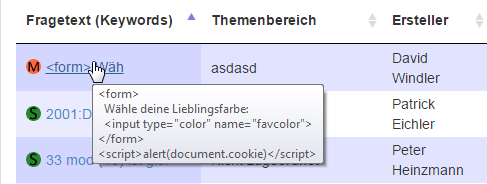
\includegraphics[width=0.7\textwidth
			]{Images/XSS_Frage.PNG}
			\caption{Platzierung des Script-Tags in der Frage}
			\cite{mobilequiz.ch}
		\end{figure}
		
		\begin{figure}[H]
			\centering
			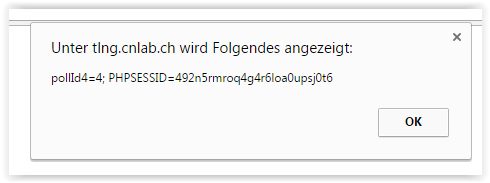
\includegraphics[width=0.7\textwidth
			]{Images/XSS_Cookie.PNG}
			\caption{Anzeige des Cookie beim Lösen der Frage}
			\cite{mobilequiz.ch}
		\end{figure}
		
		
		\item Usability \\
		In dieser Kategorie wurden die Probleme mit der Navigation und dem Auffinden von Funktionen zusammengefasst. \\
		\textit{Beispiel}: In der Lernkontrollen-Übersicht ist der Start-Button zu wenig ersichtlich.
		\begin{figure}[H]
			\centering
			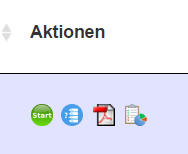
\includegraphics[width=0.20\textwidth]
			{Images/MobileQuizAlteVersionStartbutton.png}
			\caption{Ansicht der möglichen Aktionen inkl. Start-Button}
			\cite{mobilequiz.ch}
		\end{figure}
		\item Mobile-Probleme \\
		Die Kategorie beinhaltet sämtliche Probleme, welche nur in der mobilen Ansicht der Webseite vorhanden sind. \\
		\textit{Beispiel}: Der Zugriff via Smartphone auf den Profilbereich funktioniert nicht.
		\item Administrator \\
		In dieser Kategorie wurden Probleme notiert, welche nur mit Administrator-Rechten vorhanden sind. \\
		\textit{Beispiel}: Wird ein neues Themengebiet beantragt, so wird dies nicht im Log festgehalten.
		\item Probleme/Bugs \\
		In dieser Kategorie wurden alle Fehler und Probleme festgehalten, welche keiner spezifischeren Kategorie zugeordnet werden konnten. \\
		\textit{Beispiel}: Wird bei einer Lernkontrolle festgelegt, dass sie keinen Endzeitpunkt hat, so soll bei der Quiz-Teilnahme auch kein Enddatum angezeigt werden.
		\item Allgemeine Fragen zum Konzept \\
		Die Kategorie umfasst Punkte, welche zwar korrekt funktionieren, aber deren Zweck unter Umständen nicht benötigt wird. \\
		\textit{Beispiel}: Muss bei einer Registrierung wirklich die Adresse angegeben werden?
		\item Schreibfehler/Grammatik \\
		In dieser Kategorie wurden Schreibfehler oder inkonsistente Handhabungen von Ausdrücken festgehalten. \\
		\textit{Beispiel}: Der Benutzer wird wird teilweise mit \glq Sie\grq angesprochen, andernorts wird die \glq Du\grq-Form verwendet.
	\end{itemize}

	Die ausführlichen Resultate sind im Anhang unter \glqq Ergebnisse eigene Tests\grqq ersichtlich.	


	\subsection{Vergleich Online-Quizzes}
	\label{subsec:Webuntersuchungen}
	Um andere Online-Quizzes mit Mobile Quiz zu vergleichen mussten zuerst die Kriterien festgelegt werden. Als Grundlage diente eine Excel-Tabelle von Khalid Abdul und Patrik Naef, welche an die Bedürfnisse dieser Arbeit angepasst wurde. Es wurden folgende Vergleichskriterien festgelegt:
	\begin{itemize}
		\item Fragemöglichkeiten \\
		Welche Möglichkeiten bestehen eine Frage zu stellen? \\
		\textit{Beispiel:} Text mit Bild
		\item Antwortmöglichkeiten \\
		Auf welche Weise kann geantwortet werden? \\
		\textit{Beispiel:} Multiple-Choice
		\item Zeitsteuerung \\
		Gibt es Zeitbeschränkungen? \\
		\textit{Beispiel:} Festlegung der Zeit pro Frage
		\item Visuelle Signale \\
		Gibt das System Rückmeldungen an den Benutzer? \\
		\textit{Beispiel:} Rückmeldung bei Ablauf der Zeit
		\item Fragenauflösung \\
		Welche Möglichkeiten zur Punktevergabe sind vorhanden? \\
		\textit{Beispiel:} Individuelle Punktevergabe pro Frage
		\item Testfunktion \\
		Kann das Quiz vor Veröffentlichung durchgespielt werden? \\
		\item Textdarstellung \\
		Welche Einstellung können am angezeigten Text vorgenommen werden? \\
		\textit{Beispiel:} Anpassung der  Schriftgrösse
		\item Auswertungsmöglichkeiten \\
		Welche Möglichkeiten gibt es für den Ersteller das Quiz auszuwerten? \\
		\textit{Beispiel:} Auswertung pro Teilnehmer
		\item Internationalisierung \\
		Welche Möglichkeiten gibt es zur Unterstützung von mehreren Sprachen? \\
		\textit{Beispiel:} Mehrsprachige Erfassung der Quiz-Fragen
		\item Erfassen von unterschiedlichen Elementen \\
		Kann der Ersteller Kategorien, Studenten oder Gruppen erfassen?
		\item Allgemein \\
		Verschiedenen Möglichkeiten, um den Umgang mit dem Quiz zu erleichtern. \\
		\textit{Beispiel:} Erstellung eines QR-Codes zur direkten Teilnahme am Quiz
		\item Spezielle Funktionen \\
		Gibt es die Möglichkeit von Online-Kursen?
		\item Benutzerfreundlichkeit \\
		Gibt es Elemente, die dem Benutzer helfen sich leichter zurechtzufinden? \\
		\textit{Beispiel:} Schritt-für-Schritt - Erstellung eines Quizzes
	\end{itemize}
	
	\bigskip
	
	Die zu vergleichenden Websites wurden durch Google-Suchen und Empfehlungen von educatorstechnology.com \cite{educatorstechnology.com} ausgewählt.
		
	Um sicher zu sein, dass die gewählten Webseiten einen repräsentativen Anteil der Lernquizzes abdecken, wurde Kontakt mit Personen aufgenommen, welche in diesem Umfeld tätig sind. Um Unterstützung angefragt wurde bei Switch AAA, dem \acrfull{IKF} und beim \acrfull{SKMF}.
	Leider hatte bei Switch AAA niemand Zeit zur Beantwortung dieser Frage. Das \acrshort{IKF} hat selbst keine Vergleiche über bestehende Online-Quizzes, oder falls doch, handelt es sich um Unterrichtsmaterial, welches nicht herausgegeben wird. Das \acrshort{SKMF} konnte nur via ein Webformular kontaktiert werden und hat sich bis zum Ende dieser Arbeit nicht zurückgemeldet.
	
	\bigskip
	
	Die detaillierte Auswertung des Vergleichs ist im Dokument 'SA-Mobile-Quiz\_QuizSysteme-Funktionen-Vergleich-Matrix.xlsx' ersichtlich. Im Folgenden werden die wichtigsten Punkte aus dieser Analyse aufgezeigt. Es wird jeweils die Lösung im aktuellen Mobile Quiz der HSR mit der besten Lösung aus den verschiedenen Vergleichsquizzes präsentiert:
	
	\begin{itemize}
		\item Willkommensseite \\
		Webanwender haben eine riesige Auswahl an Seiten, welche auf ihr Bedürfnis zugeschnitten sind. Sie wenden deshalb nicht viel Zeit auf, um sich über eine einzelne Seite genauer zu informieren. Aus diesem Grund ist der erste Eindruck entscheidend, also eine ansprechende Willkommensseite. \\
		
		\begin{figure}[H]
			\centering
			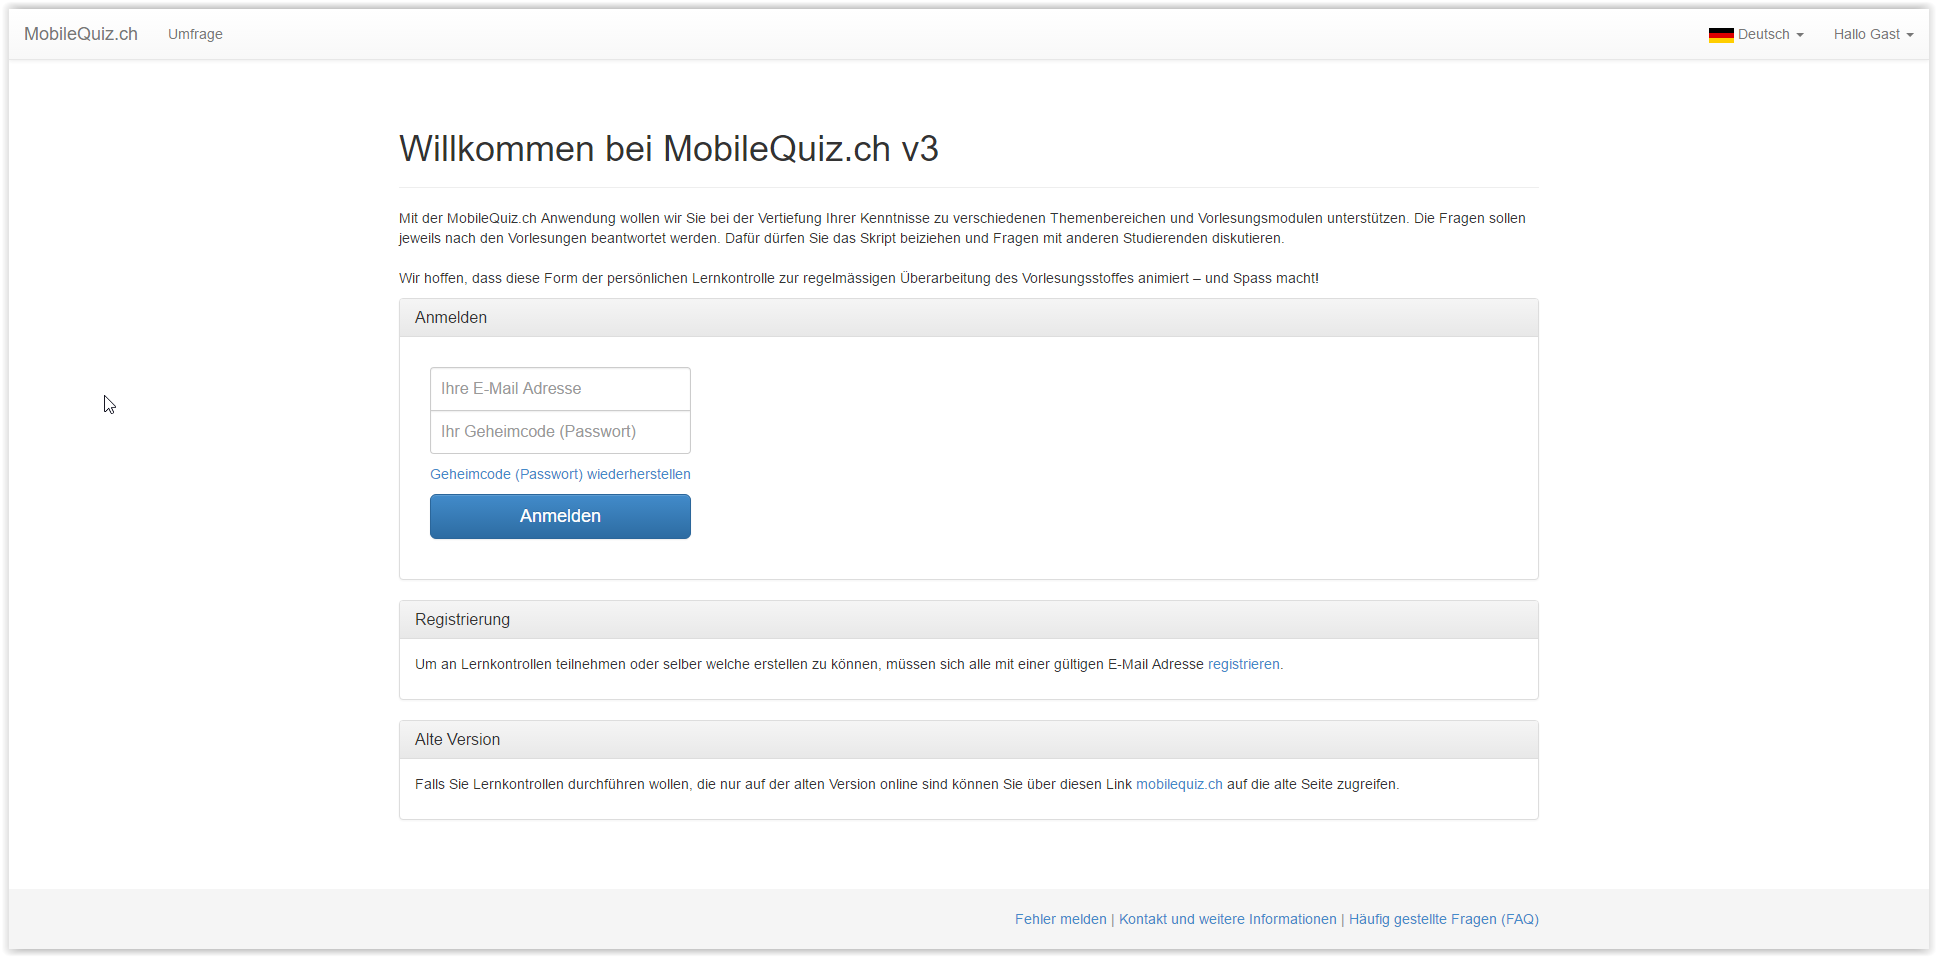
\includegraphics[width=0.75\textwidth]{Images/MobileQuiz_StartPage.PNG}
			\caption{Startseite Mobile Quiz Version 3}
			\cite{mobilequiz.ch}
		\end{figure}
		
		Ruft man www.mobilequiz.ch auf, so sieht man viel Text, der die Seite beschreibt. Ein Benutzer weiss jedoch noch nicht genau, was ihn erwartet, wenn er sich registriert und einloggt.
		
		\begin{figure}[H]
			\centering
			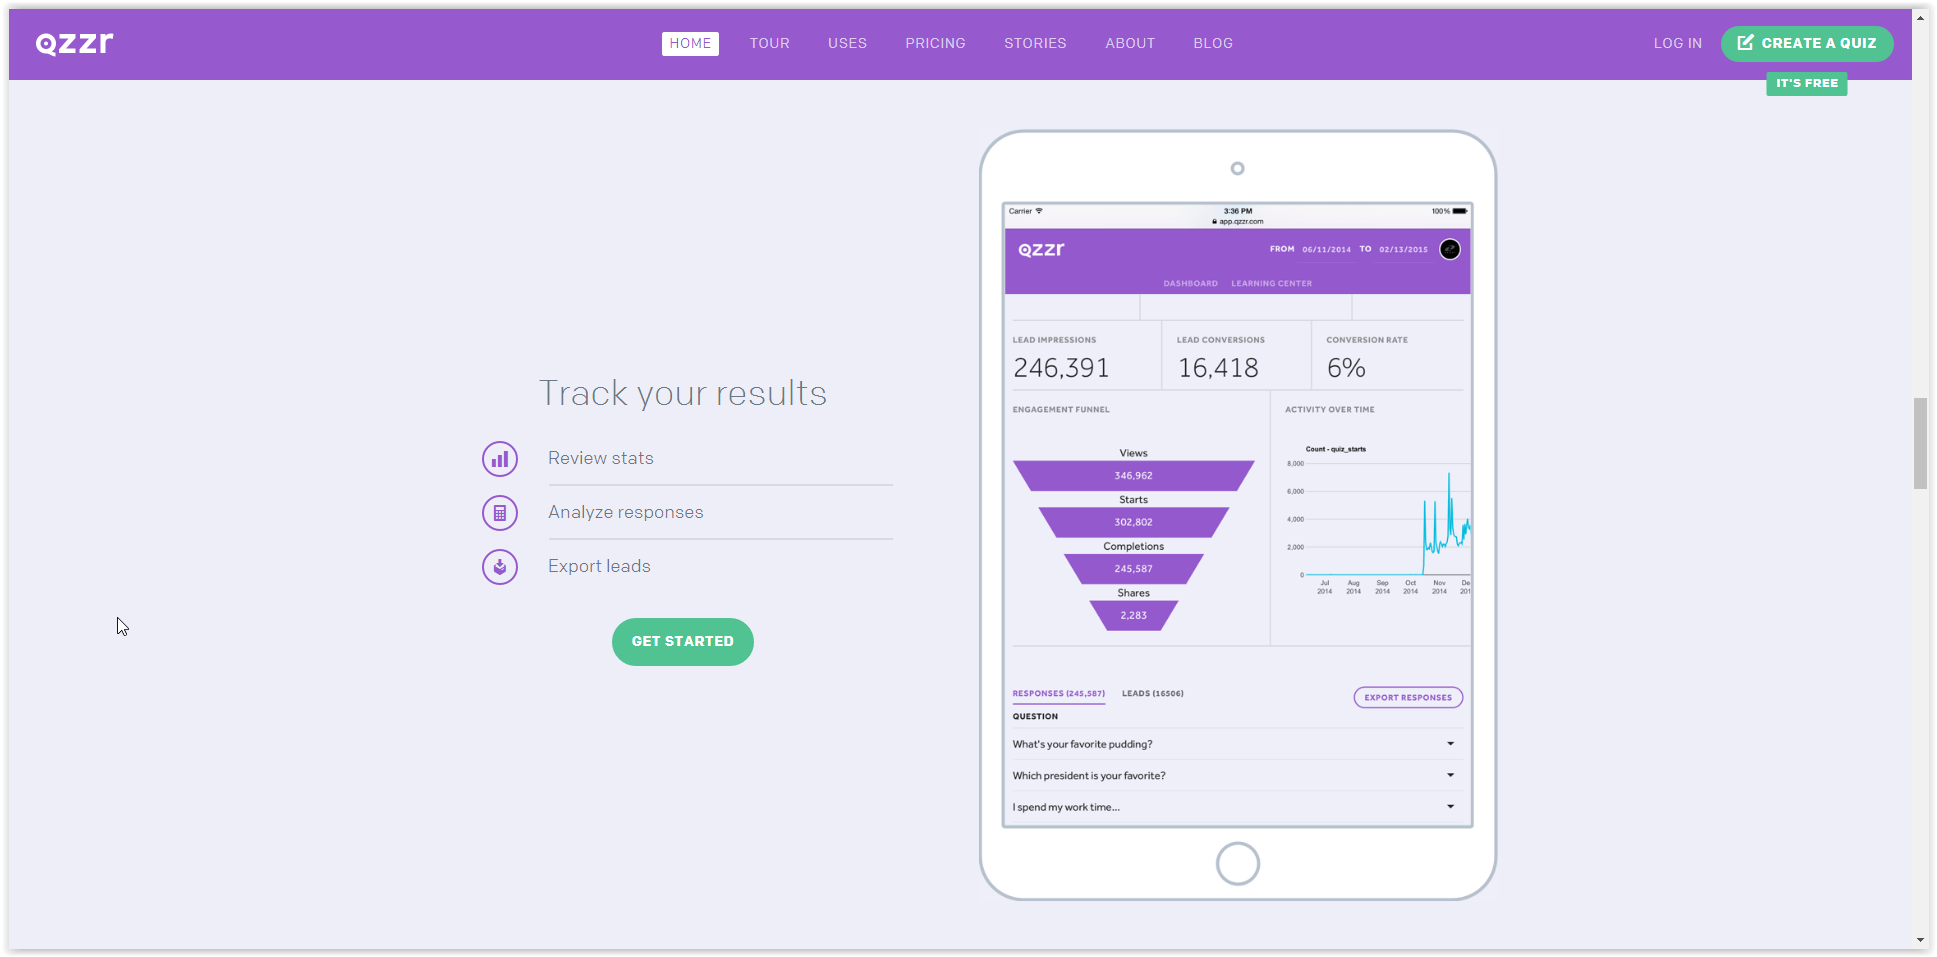
\includegraphics[width=0.75\textwidth]
			{Images/Qzzr_StartPage_Statistics.PNG}
			\caption{Startseite Qzzr}
			\cite{qzzr.com}
		\end{figure}
				
		Seiten wie Qzzr \cite{qzzr.com} hingegen, zeigen anhand von Bildern und Symbolen auf, was die Funktionalitäten sind und wie diese konkret aussehen. Solche Bilder sind schnell erfasst  und verarbeitet.
		Mobile Quiz könnte die gleichen Funktionsumfang bieten, aber wenn es der Benutzer nicht sofort sieht, klickt er weiter und registriert sich andernorts.
		
		Was machen gute Willkommensseiten also aus? \\
		Antworten darauf bietet unter anderem der Blog-Eintrag \glqq 16 of the Best Website Homepage Design Examples\grqq \cite{hubspot_kolowich} von Lindsay Kolowich.
		Aufgrund von mangelnder Zeit konnte die Willkommensseite nicht neu gestaltet werden. Dieser Punkt fliesst deshalb ins Kapitel \ref{sec:InhalteFuerStudentenarbeiten}, Inhalte für weitere Studentenarbeiten ein.
		
		
		\item Schritt für Schritt - Erstellung von Quizzes \\
		Um ein Quiz zu erstellen benötigt es einerseits die Fragen, andererseits das Quiz selbst, welches mehrere Fragen umfasst. In welcher Reihenfolge sollen diese beiden Ressourcen erstellt werden? \\
		Bei Mobile Quiz war der Ablauf so geregelt, dass zuerst die Fragen und anschliessend das Quiz separat erstellt wurde. War man sich dieser Tatsache bewusst, so stellte dies kein Problem dar, aber war es auch intuitiv? Wie in den durchgeführten Usability-Tests festgestellt wurde, war dem nicht so. Die Benutzer starteten sofort mit der Erstellung des Quizzes, mussten dann aber abbrechen, weil darin keine neuen Fragen erfasst werden konnten.
		Aus diesem Grund war es sinnvoll, diese Reihenfolge in Mobile Quiz zu ändern. Hier bot Testmoz \cite{testmoz.com} ein gutes Vorgehen:
		
		\begin{enumerate}
			\item Testnamen eingeben
			\item Testeinstellungen vornehmen
			\item Fragen erfassen
			\item Veröffentlichen
			\item Reports anschauen
		\end{enumerate}
		
		\begin{figure}[H]
			\centering
			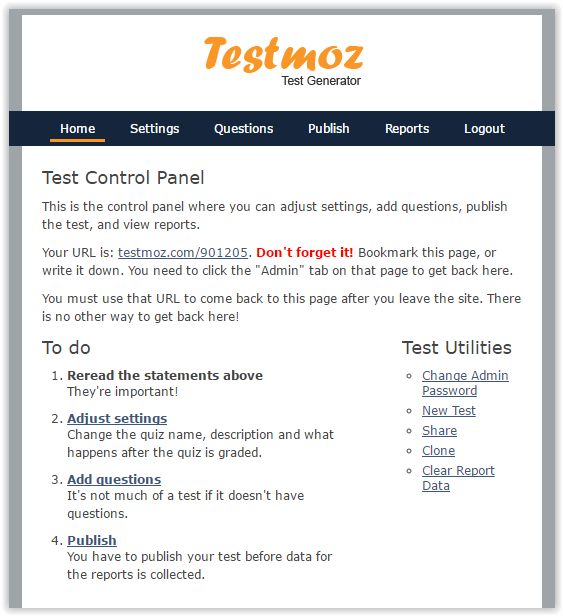
\includegraphics[width=0.4\textwidth]{Images/Testmoz2.PNG}
			\caption{Ablauf Testmoz}
			\cite{testmoz.com}
		\end{figure}
		
		Der Ablauf von Mobile Quiz war einzig darin zu ändern, dass neue Fragen während der Erstellung eines Quizzes erfasst werden können. Zur Vereinfachung konnte auch beitragen, dass der Ablauf wie bei Testmoz \cite{testmoz.com} verteilter dargestellt wird, sodass pro Seite weniger Informationen stehen. Somit findet sich der Benutzer schneller zurecht. Die genaue Beschreibung dieser Umstellung ist in Kapitel \ref{subsec:quiz-erstellung} genauer beschrieben.
		
		
		
		
		\item  Quiz-Einstellungen \\
		Quizzes können für unterschiedliche Bedürfnisse eingesetzt werden. Die möglichen Einsatzzwecke reichen von Freunden, die zum Zeitvertreib ihr Wissen gegenseitig messen wollen, über Dozenten, die prüfen möchten, ob die Studenten den Unterrichtsstoff verstanden haben, bis zu Dozenten, welche die Quizzes als Prüfung verwenden.
		Diese Situationen verlangen viele Einstellungsmöglichkeiten, welche für den Benutzer möglichst selbsterklärend sein sollen. Trifft dies jedoch nicht zu, oder ist die Darstellung unverständlich, so wird sich der Quiz-Ersteller möglicherweise nach einer anderen Quiz-Plattform umsehen.
		
		\begin{figure}[H]
			\centering
			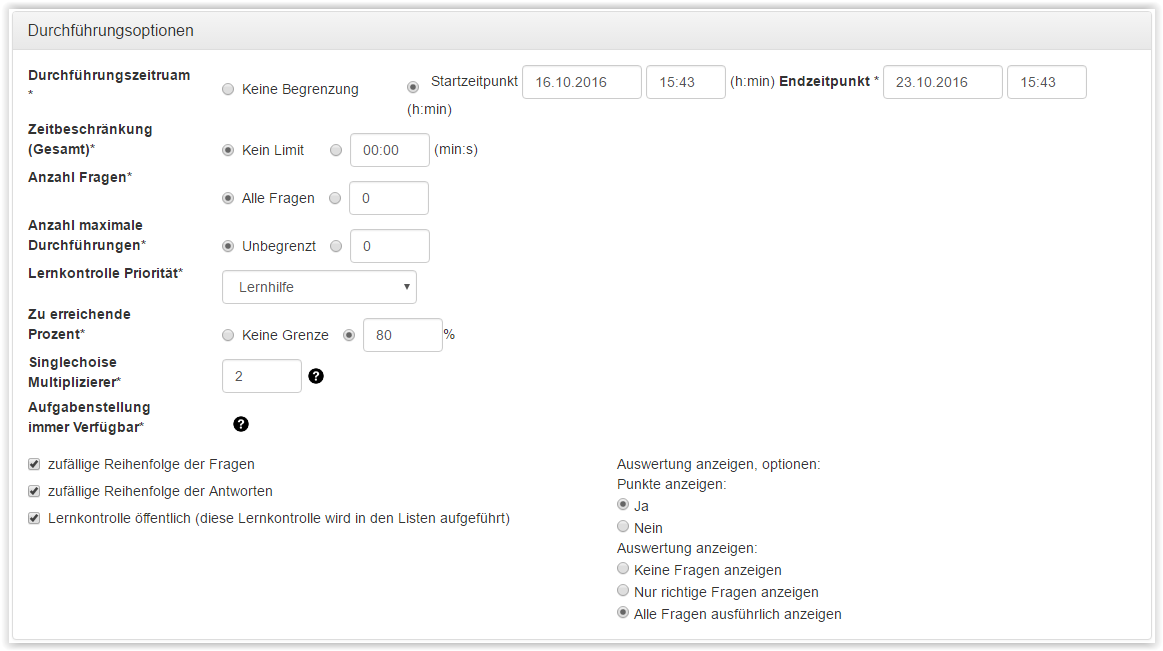
\includegraphics[width=0.75\textwidth
			]{Images/MobileQuiz_Quiz-Settings.PNG}
			\caption{Quiz-Einstellungen Mobile Quiz Version 3}
			\cite{mobilequiz.ch}
		\end{figure}
		
		
		Mobile Quiz bot zwar viele Einstellungsmöglichkeiten an, diese waren jedoch so zahlreich, dass sie den Benutzer fast überforderten. Zudem war die Darstellung zum Teil nicht optimal, da beispielsweise die 'Auswertung Anzeigen - Optionen' weiter rechts angezeigt wurde als alle anderen Einstellungen.
		
		\begin{figure}[H]
			\centering
			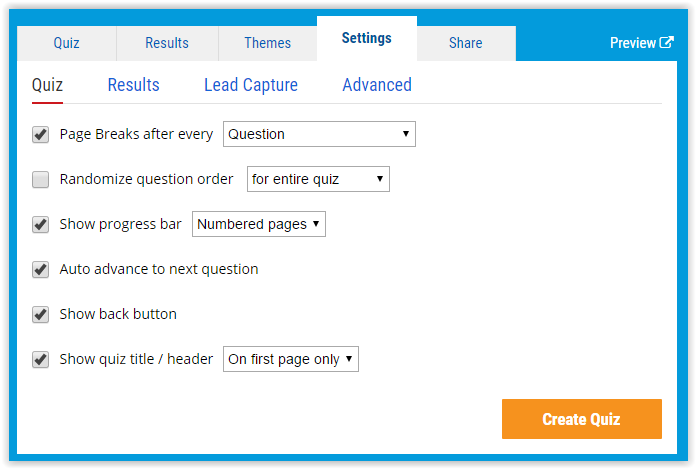
\includegraphics[width=0.5\textwidth
			]{Images/QuizMaker_Quiz-Settings.PNG}
			\caption{Quiz-Einstellungen Quiz Maker}
			\cite{quiz-maker}
		\end{figure}
		
		Aufgeräumter wirkten die Einstellungen beispielsweise bei Quiz Maker \cite{quiz-maker}. Zwar gab es ebenfalls eine Vielzahl von Möglichkeiten, diese wurden aber übersichtlich dargestellt, indem sie Themen zugeordnet und auf Tabs verteilt wurden. Zudem gab es einen eigenen Tab für erweiterte Optionen. \\
		Bei Mobile Quiz wurde der Ablauf der Quiz-Erstellung neu organisiert und in diesem Schritt auch die Quiz-Einstellungen verteilter und übersichtlicher angeordnet. Die genaue Beschreibung ist in Kapitel \ref{subsec:quiz-erstellung} vorzufinden.
		
		
		
		\item Quiz kann vor Veröffentlichung durchgespielt werden \\
		Wie sieht das erstellte Quiz für den Teilnehmer aus? Gibt es noch Rechtschreibfehler oder werden Inhalte nicht optimal dargestellt? Ein Quiz-Ersteller wird sich all diese Fragen womöglich stellen und die einfache Lösung dazu ist, dass man das Quiz vor Veröffentlichung selbst durchspielt. Die eigene Teilnahme soll jedoch nicht zählen, da sie die Auswertungsstatistik verfälschen kann. \\
		Mobile Quiz bot die Möglichkeit an, ein Quiz noch nicht zu veröffentlichen und es auf diese Weise auszuprobieren. Dies funktionierte aber nur, wenn man als Administrator eingeloggt war. Zudem zählte die eigene Teilnahme in die Gesamtauswertung mit hinein.
		Dieser Punkt konnte mangels Zeit nicht umgesetzt werden, wird aber in Kapitel \ref{sec:InhalteFuerStudentenarbeiten}, Inhalte für weitere Studentenarbeiten einfliessen.
		
		
		\item Template für Frage-Import \\
		Ist man im Zug unterwegs und möchte trotzdem an einem neuen Quiz-Fragen arbeiten, so fehlt meist der Internetzugang. Dies kompensierte Mobile Quiz dadurch, dass Fragen aus \gls{CSV}-Dateien eingelesen und erstellt werden konnten. Um dies zu nutzen, benötigte es jedoch eine spezielle Formatierung, was neue Benutzer abschrecken konnte. \\
		Die Lösung dazu war es, ein Excel-Template, also eine Vorlage, für neue Fragen bereitzustellen. Darin kann der Benutzer schnell und einfach Fragen erfassen und muss sich nicht um das Format kümmern. Solche Templates bot beispielsweise
		Socrative \cite{socrative.com} an. Es ist im Anhang unter 'socrativeQuizTemplate.xlsx' zu finden.
		
		Im Rahmen dieser Arbeit wurde ebenfalls ein solches Template erstellt, welches nun Quiz-Erstellern zum Download angeboten wird. Die genaue Beschreibung der Umstellung ist im Kapitel \ref{subsec:FrageTemplate} ersichtlich.
		
	\end{itemize}
		
	\chapter{Konzepte}
	% !TEX root = Projektdokumentation.tex

\newacronym{ICTh}{ICTh}{Informatios- und Codierungstheorie}


%Einleitung mit Erkenntniss / Zusammenfassung aus allen Unterkapiteln
Beim Erstellen der neuen Mockups wurde festgestellt, dass nebst dem Aussehen auch grundsätzliche Überlegungen zu gewissen Themen vertieft erarbeitet werden sollen. Diese Konzeptüberlegungen umfassen die Bereiche des Gruppenmanagements, der neuen Fragetypen sowie der Statistiken und den dazugehörigen Auswertungen.
In diesen Bereichen wurde Theorie erarbeitet und dann festgelegt, wie diese Konzepte umgesetzt werden können. Beim Gruppenmanagements wurden die Rollen sowie das Arbeiten mit Gruppen analysiert und erweitert. Im Bereich der neuen Fragetypen wurde zuerst theoretisch neue Frage-Formen erarbeitet und dann die Umsetzung nach Schwierigkeit und Nützlichkeit beurteilt. Schliesslich wurde bei den Statistiken mögliche neue Auswertungsformen untersucht und aufgezeigt, welche neuen Berechnungen dazu vorgenommen werden sollen.

\section{Gruppenmanagement}
In diesem Teil wurden die Rollen sowie das bestehende Gruppenmanagement angeschaut. Zu beiden Themen wurde eine Bestandsaufnahme gemacht, welche dann um sinnvolle Konzepte und Anforderungen erweitert wurde.

\bigskip

Im Bereich Rollen wurden zusätzliche Rollen definiert. Dabei handelt es sich um den Demo-User sowie um den Assistenten.

Die Rolle des Demo-Users ist dazu gedacht, dass jemand anonym die Funktionen von MobileQuiz ausprobieren kann. Nur speziell für den Demo-User gekennzeichnete Quizzes sind dabei ersichtlich und durchführbar. Eine Quiz-Durchführungen des Demo-Users wird in den Statistiken nicht erfasst.

Mit der Rolle des Assistenten wird es für einen Ersteller möglich eine oder mehrere Personen zu bestimmen, welche ebenfalls die Quizzes des Ersteller auswerten, bearbeiten und sogar in seinem Namen erstellen können. Damit wird der Situation Assistent und Dozent aus der realen Welt Rechnung getragen.

\bigskip

Die Idee der bereits bestehenden Gruppen wurde so erweitert, dass ein Teilnehmer neu mehr als einer Gruppe zugewiesen werden kann.

Zudem kann ein Quiz neu mehrere Durchführen haben. Die Festlegung des Durchführungszeitraum sowie des Quiz-Typs wird aus dem Quiz in die Durchführung verschoben. Damit ist es möglich, das Quiz einmal zu erstellen und es dann aufgrund der gewählten Durchführungszeiträume und Quiz-Typen als unterschiedliche Durchführungen laufen zu lassen. Die Durchführung wird so konzipiert, dass ihr entweder eine Gruppe oder ein einzelner Teilnehmer hinzugefügt werden kann. 

\bigskip

Die ausführliche Ausarbeitung aller Ergebnisse ist im Anhang im Dokument 'Strukturierte\_Gruppenadministration\_AnforderungenV2.doxc' ersichtlich. Zudem finden Sie sämtliche Datenbankanpassungen, welche für diese Änderungen notwendig sind, im Dokument \\'DB\_nach\_Änderungen\_Assistant-has-1-CreatorV2.pdf'.


\section{Neue Fragetypen}
Für dieses Konzept wurde zuerst die Theorie zu unterschiedlichen Fragetypen erarbeitet. Danach wurde beurteilt, welche neuen Fragetypen wie schwierig umzusetzen sind und wie nützlich sie für MobileQuiz sind. Zudem wurde ein neues Excel-Template entwickelt, dessen detaillierte Beschreibung unter 12.1.1 'Frage-Template' ersichtlich ist.

\bigskip

\noindent Es wurden folgende Fragetypen als mögliche neue Fragetypen angeschaut:
\begin{itemize}
	\item Single-Choice und Multiple-Choice - Fragen mit Bildern als Antwort
	\item Single-Choice und Multiple-Choice - Fragen mit Bild in der Frage
	\item Freitext
	\item Lückentext
	\item Lückentext mit DropDown Auswahl
	\item Drag \& Drop
	\item Antworten Sortieren
	\item Code-Evaluation
\end{itemize}

\bigskip

Davon wurden die folgenden weiterverfolgt:
\begin{itemize}
	\item Single-Choice und Multiple-Choice - Fragen mit Bild in der Frage:
	Dieser Fragetyp wird beispielsweise bei \acrshort{CN1} verwendet, um Fragen zu einem Netzwerklayout zu stellen.
	\item Freitext:
	Dieser Fragetyp nicht implementiert, diente er als Inspiration für ein Feedback-Feld unter jeder Frage. Ist eine Frage für einen Studenten nicht verständlich, so kann er seine Frage über dieses Feld direkt an den Quiz-Ersteller senden.
	\item Antworten Sortieren:
	Dieser Fragetyp wäre beispielsweise bei \acrshort{CN1} nützlich, um Netzwerktechnologien nach Geschwindigkeit zu ordnen.
	\item Drag \& Drop:
	Dieser Fragetyp wäre für \acrshort{CN1} und \acrshort{ICTh} attraktiv, beispielsweise für die Bezeichnungen von Übertragungsverfahren.
\end{itemize}

\noindent Für die weiteren Fragetypen besteht derzeit kein Bedarf, worauf auf die Umsetzung verzichtet wird.

\bigskip

Sämtliche Überlegungen zu diesem Kapitel befinden sich im Dokument \\ 'Strukturierte\_Fragetypen\_AnforderungenV2.docx', die dazu notwendigen Datenbankänderungen sind im Dokument 'newQuestions\_MobileQuizDB.mdj' festgehalten.
Das neu erarbeitete Excel-Template ist unter 'Umsetzungsvorschlag\_Frage\_TemplateV2.xlsx' ersichtlich.

\section{Statistiken und Auswertungen}
In den Statistiken und Auswertungen wurden neue Auswertungstypen angeschaut und beurteilt, welche davon umgesetzt werden sollen. Zudem wurde ausgearbeitet, wie die neuen Auswertungen zugänglich sein sollen.

\bigskip

\noindent Dabei handelt es sich um folgende neue Statistiken:
\begin{itemize}
	\item Anzahl der Teilnahmen
	\item Mittelwert
	\begin{itemize}
		\item für Punkte
		\item für Zeit
	\end{itemize}
	\item Standardabweichung
	\begin{itemize}
		\item für Punkte
		\item für Zeit
	\end{itemize}
	\item Aufgabenschwierigkeit
	\item Risikobereitschaft
	\item Discrimination Index
\end{itemize}

Die genaue Erläuterung sowie die Berechnung finden Sie im Dokument \\ 'Strukturierte\_Statistiken\_AnforderungV2.docx'. Die dazu nötigen Datenbankänderungen sind im Dokument 'newStatistiken\_MobileQuizDB.pdf' dokumentiert.
















	
	
	
	\chapter{Software Engineering}
	%Software Engineering: Systembeschreibung, Software-Architektur, Domainmodell, Sequenzdiagramme, etc. (Anhand dieses Teils sollte man genau verstehen, was wie realisiert wurde. Informatiker sollten alle für die Optimierung oder Weiterentwicklung des System nötigen Informationen haben.)
	%Überarbeitung gewisser Konzepte, Bspw. Teilnahme
	% !TEX root = Projektdokumentation.tex


\section{Datenbankänderung}

\subsection{Bestehende Datenbank}

Für die Behebung der bestehenden Fehlern sowie für die Erstellung neuer Funktionalitäten war es wichtig, einen exakten Überblick über die Datenbank zu besitzen. Da zu Beginn nur eine veraltete Übersicht über die Tabellen vorhanden waren, musste diese zuerst aktualisiert werden. Die erstellte Übersicht ist im Anhang unter \glqq Datenbank aktueller Zustand \grqq auf Seite \hyperlink{page.\getpagerefnumber{pdf:dbVorVeraenderung}}{\getpagerefnumber{pdf:dbVorVeraenderung}} zu finden.



\subsection{Änderung an der Datenbank}
\label{subsec:DBAenderungen}
Verschiedene neue Funktionalitäten verlangten eine Änderung der Datenbank, da neue Arten von Daten abgespeichert werden mussten.


\begin{figure}
	\centering
	\begin{subfigure}{.5\textwidth}
		\centering
		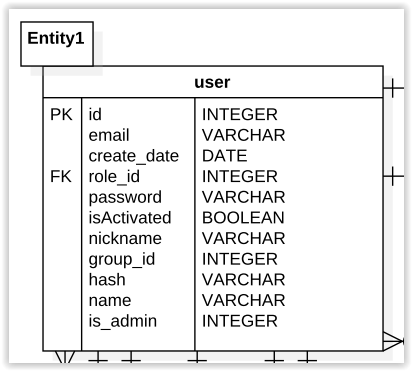
\includegraphics[width=0.6\textwidth]{Images/DB_User_Table.PNG}
		\caption{Alte User-Tabelle}
	\end{subfigure}%
	\begin{subfigure}{.5\textwidth}
		\centering
		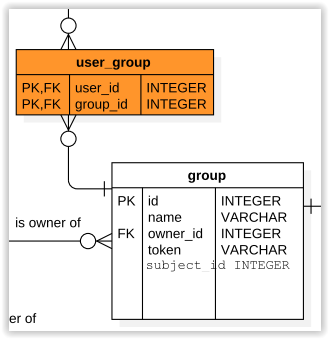
\includegraphics[width=0.6\textwidth]{Images/DB_Group_Table.PNG}
		\caption{Neue user\_group - Beziehung}
	\end{subfigure}
\end{figure}



\begin{itemize}
	\item Gruppenmanagement\\
	Ein Benutzer konnte bisher nur einer Gruppe zugeordnet sein. Wie auf dem Bild a) ersichtlich, war deren ID direkt in der Tabelle \glqq User\grqq gespeichert. Neu sollte eine Gruppe mehrere Benutzer beinhalten und ein Benutzer in mehreren Gruppen sein können. Es wurde deshalb, wie auf Bild b) ersichtlich, eine Zwischentabelle für die Auflösung der N:M - Beziehung gemacht.\\
	Mehrere Gruppen werden unter anderem dafür benötigt, dass ein Benutzer neu seine\\ Themenbereich-Interessen angeben kann und dafür je einer Gruppe zugeordnet ist. Dazu kommen die Praktikums- und Vorlesungsgruppen.
	\item Quiz-Durchführungen\\
	Da es im Modul \gls{CN1} mehrere Praktikumsgruppen gibt, welche unterschiedliche Zeiträume für die Lösung von Quizzes zur Verfügung haben, benötigte es pro Quiz mehrere Durchführungen.
	
	Neu können mehrere Durchführungen erstellt und zu diesen Gruppen zugeordnet werden. So kann ein Enddatum pro Gruppe festgelegt werden.
	Dafür mussten in der Datenbank einige Änderungen vorgenommen werden. 
	
	Die Wichtigste dieser Änderungen war das Erstellen der \glqq execution\grqq - Tabelle. Die bisherigen Einstellungen für eine Durchführung eines Quizzes wurden aus der Tabelle \glqq questionnaire\grqq in die Tabelle \glqq execution\grqq übertragen.
	
	Es wurden mehrere Verknüpfungstabellen nötig, welche dafür sorgen, dass Quizzes, Teilnehmer und Gruppen einer Durchführung zugeordnet werden können.
	
	Schlussendlich wurde die Tabelle \glqq priority\_settings\grqq erstellt. In dieser werden vom Standard abweichende Einstellungen eines Erstellers abgespeichert. Bei der Erstellung einer neuen Durchführung wird überprüft, ob solche Werte vorhanden sind. Wenn ja, werden diese für die neue Durchführung eingetragen, wenn nein, werden die vordefinierten Standard-Einstellungen von Mobile Quiz verwendet. Das Ziel dahinter ist, dass der Ersteller so wenig wie möglich von Hand einstellen muss, sobald er seinen Durchführungstyp beziehungsweise seine Durchführungspriorität (Lernhilfe, Testatbedingung, Prüfung) gewählt hat.
	
	In der untenstehenden Grafik sind alle Datenbankänderungen festgehalten. Dabei sind die neu erstellten Tabellen orange ausgefüllt und die veränderten Tabellen orange umrahmt.
	
	\begin{figure}[H]
		\centering
		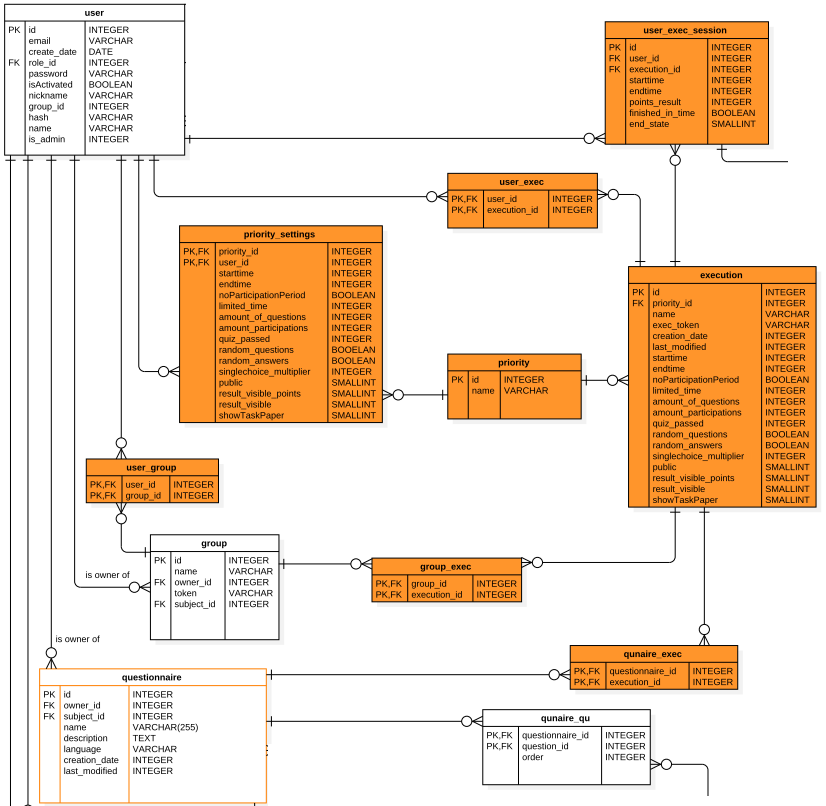
\includegraphics[width=1\textwidth
		]{Images/DB_Execution_Table.PNG}
		\caption{Datenbankänderungen für die Durchführung}
	\end{figure}
	
\end{itemize}

Diese umfangreichen Datenbank-Änderungen zogen viele Anpassungen von Datenbankabfragen nach sich, da beim bisherigen \glqq questionnaire\grqq viele Verbindungen zusammenliefen. So musste von der Quiz-Erstellung, über die Quiz-Durchführung bis zur PDF-Generierung der Auswertung vieles umgeschrieben werden.
	
	
	
	
	\chapter{Realisierung}
	%Realisierung, System- oder Softwarekonzepte
	%Umsetzung von neuen Konzepten und Desgin
	% !TEX root = Projektdokumentation.tex

\newglossaryentry{XML External Entitiy} {name={XML External Entitiy-Attacke},description={Eine Attacke, welche gegen einen XML-Input-Parser geht. Sie tritt auf, wenn der XML-Input einen Verweis auf eine externe Server-Ressource enthält, auf welche der Angreifer gar keinen Zugriff haben dürfte, und der Parser dies nicht prüft. \cite{xxe}}}

\newglossaryentry{Refactoring}{name={Refactoring},
	description={Refactoring bezeichnet die manuelle oder automatisierte Strukturverbesserung von Quelltexten unter Beibehaltung des beobachtbaren Programmverhaltens. Dabei sollen die Lesbarkeit, Verständlichkeit, Wartbarkeit und Erweiterbarkeit verbessert werden, mit dem Ziel, den jeweiligen Aufwand für Fehleranalyse und funktionale Erweiterungen deutlich zu senken. \cite{_refactoring_2016}}
}

\newglossaryentry{URL}{name={URL},description={\begin{quote}
			Uniform Resource Locator (URL) ist eine Adressierungsform für Internetadressen, die vor allem innerhalb des World Wide Web (WWW) zur Anwendung kommt.
		\end{quote} \cite{url}}}

\newglossaryentry{Denial of Service}{name={Denial of Service},description={\begin{quote}
			\glqq Durch einen Denial-of-Service (DoS)-Angriff werden Dienste in ihrer Funktionalität beeinträchtigt und stehen Nutzern sowie Unternehmen nur eingeschränkt zur Verfügung.\grqq
		\end{quote} \cite{dos}}}

\newacronym{AJAX}{AJAX}{Asynchronous Javascript And XML}



\section{Verbesserung der bestehenden Lösung}

\subsection{\gls{Refactoring} und Fehlerbehebung}

Aufgrund der im Kapitel \ref{subsec:eigeneUntersuchungen} vorgenommenen eigenen Untersuchungen von Mobile Quiz entstand eine Liste von zu behebenden Problemen. Diese detaillierte Liste ist im Dokument \glqq Ergebnisse eigene Tests\grqq ab Seite \hyperlink{page.\getpagerefnumber{pdf:eigeneTests}}{\getpagerefnumber{pdf:eigeneTests}} ersichtlich. In diesem Kapitel werden die wichtigsten vorgenommenen Änderungen angeschaut.

\begin{itemize}
	\item Es wurden unterschiedliche Fehlermeldungen bei falscher E-Mail Adresse oder falschem Passwort ausgegeben. Dies wurde aus Sicherheitsgründen geändert, da es einem Angreifer Aufschluss über korrekte E-Mail - Adressen gibt. Es wird neu bei einer falschen Eingabe von Passwort oder E-Mail folgende generelle Meldung angezeigt:	
	\begin{figure}[H]
		\centering
		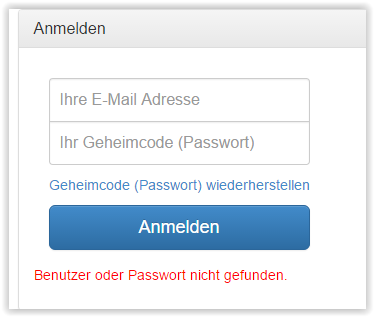
\includegraphics[width=0.5\textwidth]
		{Images/nachher_Email-und-Passwort.PNG}
		\caption{Neu umgesetzte Fehlermeldung}
	\end{figure}

	\item Wenn während einer Quiz-Teilnahme versucht wurde, das Quiz durch klicken auf den Abbrechen-Button zu verlassen, führte das teilweise zu keiner Aktion. An was dies lag, ist in folgendem Bild gut ersichtlich. Es wurde nur innerhalb der blauen Markierung auf die Klicks von Benutzer reagiert. Dieser blaue Ausschnitt war jedoch verschoben und wurde als Korrekturmassnahme direkt über dem Abbrechen-Button platziert.
	
	\begin{figure}[H]
		\centering
		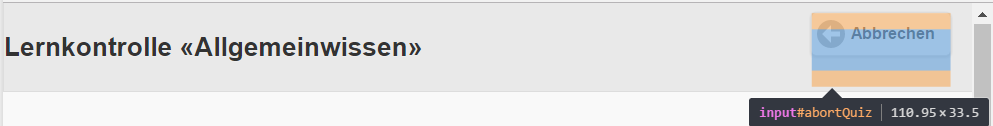
\includegraphics[width=0.75\textwidth]
		{Images/CancelButtonProblem.PNG}
		\caption{Screenshot des Problems des Abbrechen-Buttons}
		\cite{mobilequiz.ch}
	\end{figure}
	
	\begin{figure}[H]
		\centering
		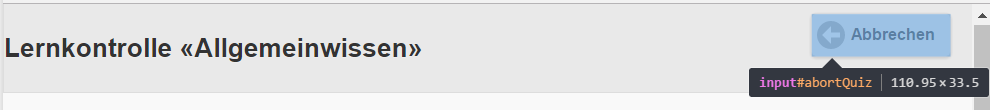
\includegraphics[width=0.75\textwidth]
		{Images/CancelButtonFix.PNG}
		\caption{Screenshot der Lösung für das Problem des Abbrechen-Buttons}
	\end{figure}
	
	\item Es wurden diverse Verbesserungen im HTML vorgenommen. Zum Beispiel waren im Registrierungsformular sämtliche Input-Typen auf 'text' gesetzt. Diese wurden entsprechend dem erwarteten Eingabetyp angepasst.
	
	Zudem wurde der Doctype-Tag von HTML4 auf HTML5 aktualisiert. Dieser Doctype-Tag teilt dem Browser mit, in welcher Version das HTML geschrieben ist und wie er das Dokument zu interpretieren hat.
	
	\item An den wichtigsten Stellen wurde die gefundene \gls{Cross-Site-Scripting} Schwachstelle behoben. Es gibt allerdings noch Stellen im Mobile Quiz an denen diese Schwachstelle nicht behoben wurde. Grundsätzlich müsste jedes Element welches von einem Benutzer (sei es Teilnehmer, Ersteller, Assistent oder Administrator) eingegeben wurde bei seiner Ausgabe so codiert werden, dass es nicht mehr ausgeführt werden kann. Wenn dies nicht gemacht ist, kann ein böswilliger Benutzer von ihm erstellten Code ausführen lassen. Dies kann im schlimmsten Fall zum Verlust von Benutzerdaten und Sessions führen. Damit kann ein Angreifer dann im Namen von anderen Benutzer im System agieren.
	
	\item Bei der Durchführung eines Quizzes wird oben links im Stil X/Y jeweils angezeigt, bei welcher Frage X der totalen Anzahl zu beantwortenden Fragen Y man sich befindet. Allerdings hatte es einen Fehler in der Logik, es wurde beim Zurück-Navigieren ebenfalls nach oben gezählt, womit die Aussage nicht mehr stimmte.
	Die Logik wurde so angepasst, dass dieser Zähler nun in jedem Fall korrekt berechnet wird. 
	
\end{itemize}


\subsection{Frage-Template}

\label{subsec:FrageTemplate}
Die Möglichkeit, Fragen offline zu erstellen und anschliessend hochzuladen, bestand bereits. Unterstützt wurde die Erfassung von Singechoice und Multiplechoice-Fragen. Dazu konnten Fragen in eine \gls{CSV}-Datei geschrieben werden. Alle korrekten Antworten wurden mit einem Asterisk (Stern-Zeichen) versehen. Eine Multiplechoice-Frage lag vor, wenn mehr als eine Antwort mit einem Asterisk versehen war.

In dieser Arbeit wurde das CSV-Template durch ein Excel-Template abgelöst. Die Gründe dazu sind die folgenden:
\begin{itemize}
	\item Die Regeln für das Erstellen waren einem kleinen Personenkreis bekannt. Sie wurden auf der Webseite nicht beschrieben. Damit die Funktion aber Verbreitung findet, muss die Vorgehensweise öffentlich zugänglich sein.
	
	Es wurde entschieden, ein Excel-Template zum Download auf der Webseite anzubieten. Darin sind alle relevanten Informationen für die Erstellung vorhanden.
	
	\item Werden die Fragen in Excel erstellt und anschliessend daraus eine CSV-Datei generiert, so hat man die Wahl zwischen 3 verschiedenen CSV-Varianten.
	
	Der Excel-Import hingegen unterstützt alle Excel-Dateien mit der Endung .xlsx. Dieses Format ist ab Excel 2007 das Standardformat und daher weit verbreitet.
	\cite{microsoft2016}
	
	\item Das CSV-Template war auf Singlechoice und Multiplechoice - Fragen beschränkt.
	
	Da neue Fragetypen unterstützt werden sollten, wurde eine neue Struktur mittels Excel erarbeitet. Um den Ersteller zu Unterstützen wurde mit Farben und weiteren Funktionen gearbeitet, welche durch CSV nicht unterstützt werden.

\end{itemize}

Durch den Einsatz des neuen Templates konnte auch ein Umlaute-Bug behoben werden, welcher aufgrund des CSV-Templates entstand. Bei der Erstellung von Fragen wird geprüft, ob die gleiche Frage bereits schon besteht. Falls dies der Fall ist, wird beim Quiz die bestehende Frage hinzugefügt und keine neue erstellt. Mit dem CSV-Template gab es einen Fehler bei der Erkennung von Umlauten, wodurch es zu Doppel-Erstellungen kam. Mit dem neuen Excel-Template geschieht dies nicht mehr.

\bigskip

Ein Beispiel des ursprünglichen Formats sowie des neuen Excel-Templates ist im Anhang, im Kapitel 19 \glqq Details zur Lösungsfindung\grqq auf den Seiten \hyperlink{page.\getpagerefnumber{pdf:csvTemplate}}{\getpagerefnumber{pdf:csvTemplate}} und \hyperlink{page.\getpagerefnumber{pdf:excelTemplate}}{\getpagerefnumber{pdf:excelTemplate}}, ersichtlich.

\bigskip

Der neue Template-Import wurde mit PHPExcel \cite{phpexcel} umgesetzt. Diese PHP-Library war bereits im Projekt eingebunden und wird dazu verwendet, die Rangliste aller Teilnehmenden eines Quizzes in eine Excel-Datei zu Exportieren. Die neue Logik befindet sich hauptsächlich in der neu erstellen Datei \glqq importExcel.php\grqq.

\bigskip

Bei PHPExcel gab es bis zur Version 1.7.9 eine \gls{XML External Entitiy} - \gls{Vulnerability}. Dadurch war es Remote-Angreifern möglich, beliebige Dateien auf dem Server zu lesen oder eine \gls{Denial of Service} - Attacke durchzuführen. \cite{cvedetails_phpexcel}
Da bei Mobile Quiz allerdings die Version 1.8.0 verwendet wird, ist dies nicht mehr möglich. Es wurde mit dem Wissen aus dem Fach Informationssicherheit 3 versucht eine solche Attacke durchzuführen, was ebenfalls zum Ergebnis führte, dass diese Sicherheitslücke nicht mehr vorhanden ist.



\subsection{Ablauf Quiz-Erstellung}
\label{subsec:quiz-erstellung}

Um in Mobile Quiz ein Quiz zu erstellen war es bisher so, dass zuerst die Fragen und anschliessend das Quiz separat erstellt werden musste. Dieser Ablauf war nicht nur bei der eigenen Untersuchung der Webseite unklar, er warf auch bei den Usability-Tests Fragen auf. Dabei versuchten die Teilnehmer oft ein Quiz zu erstellen und wollten darin die Fragen erfassen. Da dies auch der Standard-Ablauf aller anderen untersuchten Quiz-Webseiten war, wurde er auch in Mobile Quiz implementiert.

Wie auf der unteren Abbildung ersichtlich ist, werden nun zuerst die allgemeinen Informationen erfasst, welche bei jeder Quiz-Durchführung gleich sein sollen. Anschliessend können im Frage-Tab neue Fragen erstellt oder bestehende zum Quiz hinzugefügt werden. Schliesslich können eine oder mehrere Durchführungen erstellt werden.

\begin{figure}[H]
	\centering
	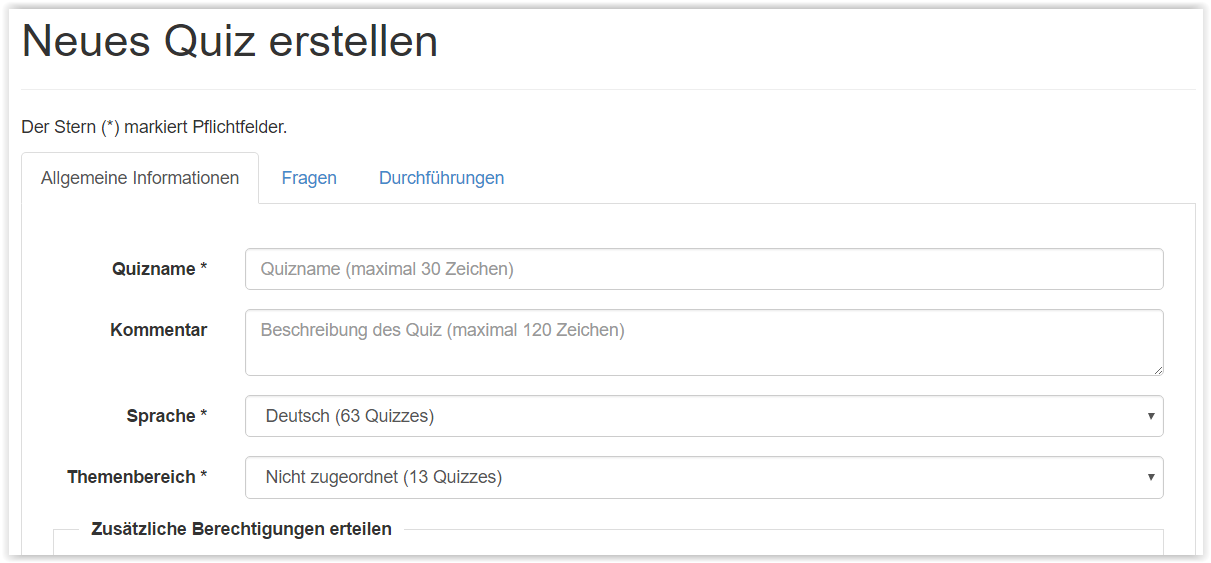
\includegraphics[width=0.8\textwidth]{Images/Quiz_Erstellen1.PNG}
	\caption{Neuer Ablauf der Quiz-Erstellung}
\end{figure}

Das Konzept der Durchführungen wurde in diesem Projekt neu erarbeitet und entstammte aus dem Wunsch, Quizzes für die einzelnen \acrshort{CN1}-Praktikumsgruppen anzupassen. Dabei nehmen die Studenten, in immer der gleichen Gruppe, jeweils im zwei-Wochen-Takt am Praktikum teil. Es gibt sowohl in der ersten als auch in der zweiten Woche mehrere Praktikumsgruppen.

Nach dem Praktikums wird das Gelernte mit einem Online-Quiz überprüft. Dieses soll aber erst nach dem Praktikum und nur eine Woche lang aufgeschaltet sein. Dies konnte mit der bestehenden Mobile Quiz - Version nur mit Mehraufwand umgesetzt werden, da der festgelegte Durchführungszeitraum für alle Gruppen gleich war. Unterschiedliche Termine konnten nur festgelegt werden, indem mehrere Quizzes mit entsprechenden Datumsbeschränkungen erstellt wurden.

\bigskip\bigskip

\textbf{Lösung}
\bigskip

Neu ist es für solche Fälle möglich, ein Quiz mit mehreren Durchführungen zu erstellen. Das Quiz selbst umfasst nur noch Eigenschaften wie der Name oder die Sprache, welche bei jeder Durchführung gleich sind. Ebenfalls werden die Fragen mit dem Quiz verknüpft. Anschliessend ist es möglich, für das Quiz mehrere, unterschiedliche Durchführungen zu erstellen. Diese beinhalten Einstellungen wie zum Beispiel den Start- und Endzeitpunkt sowie die zugewiesenen Gruppen und Teilnehmer.


\begin{figure}[H]
	\centering
	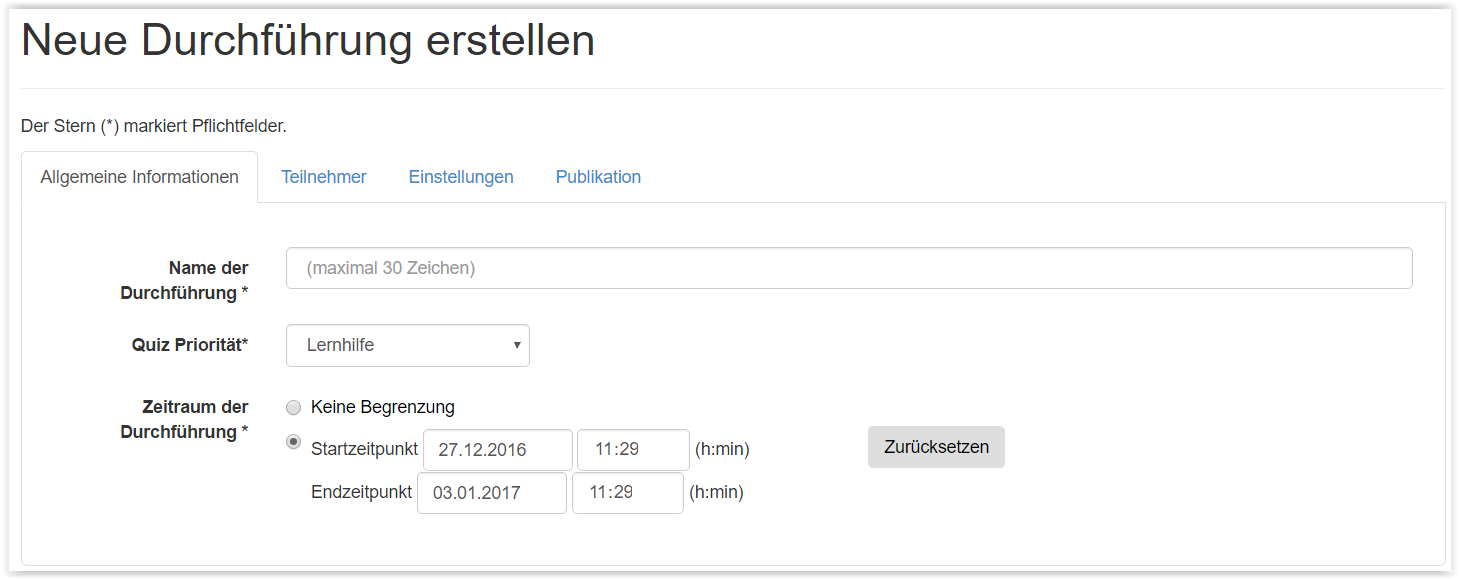
\includegraphics[width=0.8\textwidth]{Images/Quiz_Durchfuehrung1.PNG}
	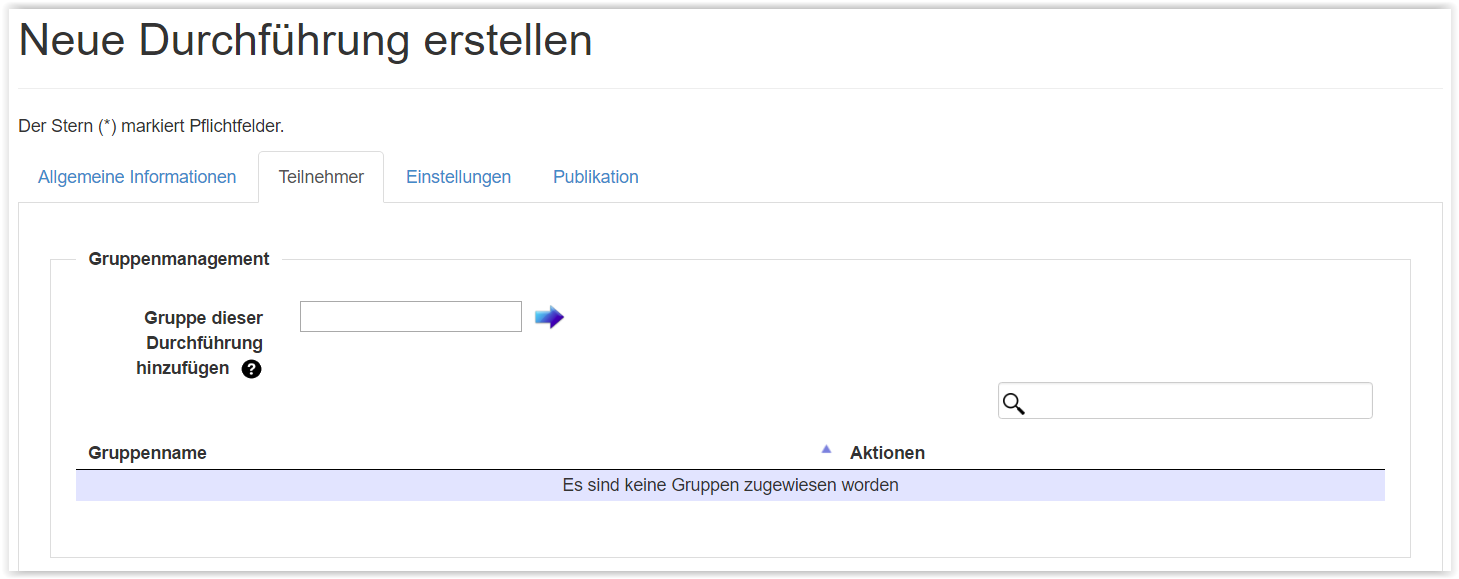
\includegraphics[width=0.8\textwidth]{Images/Quiz_Durchfuehrung2.PNG}
	\caption{Erfassung einer Durchführung}
\end{figure}


Auf diese Weise bietet Mobile Quiz für die oben beschriebene Situation eine einfache Lösung an. Das Quiz selbst muss nur noch einmal erstellt werden. Für die Praktikumsgruppen der ersten Woche wird dann eine Durchführung für den Zeitraum einer Woche nach dem Praktikum erfasst und die Gruppen zugewiesen. Das gleiche gilt für die Praktikumsgruppe der zweiten Woche. \\

\bigskip\bigskip

\textbf{Weitere Vereinfachungen}
\bigskip

Mobile Quiz geht hier allerdings noch einen Schritt weiter. Schon in der bestehenden Version gab es drei Quiz-Prioritäten, nämlich Lernhilfen für Unterrichtsfragen, Lernkontrollen für Testate und Prüfungen. Jede dieser Prioritäten besitzt bereits vordefinierte Einstellungen, welche automatisch gesetzt werden, wenn bei der Quiz-Erstellung die Priorität gewechselt wird. So ist zum Beispiel die maximale Anzahl Teilnahmen bei einer Prüfung immer eins. Somit wird der Ersteller davon befreit, alle Einstellungsmöglichkeiten selbst zu setzen. Möchte er trotzdem einzelne Werte verändern, so werden diese neuen Werte in der Datenbank in seinem Profil abgespeichert. Bei jeder nachfolgenden Quiz-Erstellung wird dann geprüft, ob beim Ersteller solche Werte gespeichert sind. Falls dies nicht der Fall ist, werden wieder die vordefinierten Default-Werte verwendet. Die mit Herr Heinzmann besprochenen Default-Werte sind im Anhang unter \glqq Default-Einstellungen\grqq auf Seite \hyperlink{page.\getpagerefnumber{pdf:defaultEinstellungen}}{\getpagerefnumber{pdf:defaultEinstellungen}} ersichtlich.

\bigskip\bigskip

Aufgrund von fehlender Zeit konnte die Implementierung der Durchführungs-Erstellung nicht abgeschlossen werden. Dieser Punkte wurde deshalb in den noch nicht fertiggestellten Arbeiten \ref{subsec:NichtFertiggestellteArbeiten} aufgeführt.





\subsection{Design Quiz- und Frage-Erstellung}
Bei der ersten Durchführung der \gls{Usability-Test}s stellte sich heraus, dass die Teilnehmer von den Einstellungsmöglichkeiten teilweise überfordert waren. Dies lag vor allem daran, dass sehr viele Optionen auf einmal angezeigt wurden und diese zudem unstrukturiert, auf der ganzen Seite verteilt, dargestellt wurden.


\begin{figure}[H]
	\centering
	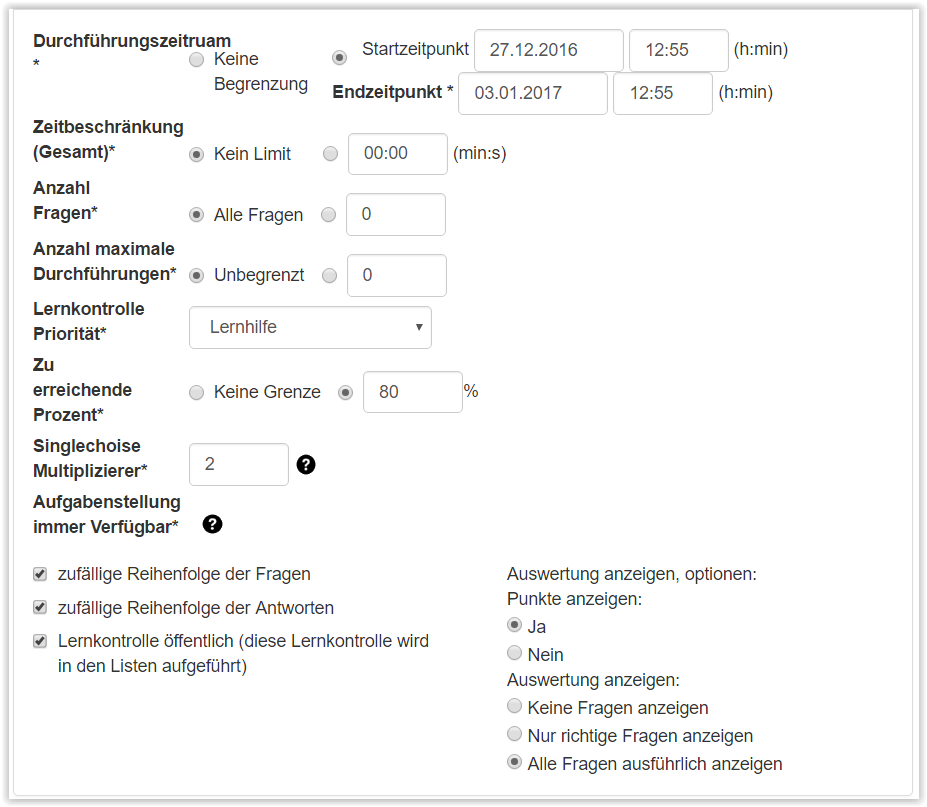
\includegraphics[width=0.6\textwidth]{Images/Einstellungen_alt.PNG}
	\caption{Einstellungsmöglichkeiten der bestehenden Mobile Quiz - Version 3}
	\cite{mobilequiz.ch}
\end{figure}


Um dem entgegenzuwirken wurde die Quiz-Erstellung auf mehrere Seiten aufgeteilt, welche thematisch zusammengehören. Diese Seite werden in einzelnen Tabs dargestellt. Da Tabs auf mobilen Geräten nicht immer gut dargestellt werden, wurde ein Design gesucht, welches die Inhalte in dieser Ansicht optimal anzeigt. Dieses wurde mit dem Accordion-Design gefunden.


\begin{figure}[H]
	\centering
	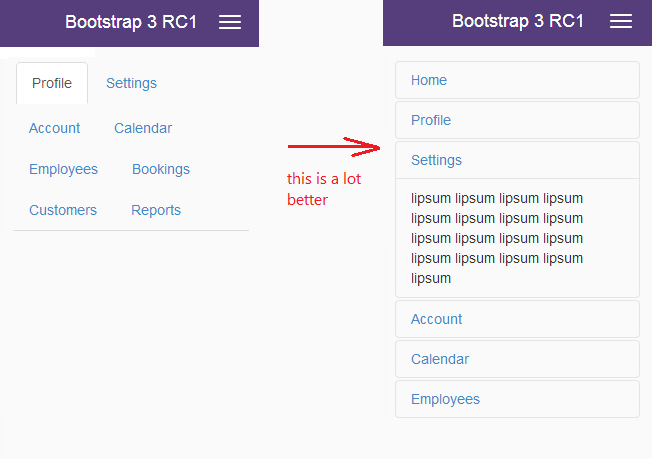
\includegraphics[width=0.6\textwidth]{Images/Bootstrap_Accordion.png}
	\caption{Tabs im Vergleich zum Accordion - Design}
	\cite{tabs_accodion}
\end{figure}

Um nun beide Ansichten zu vereinen wurde \glqq Bootstrap Tab Collapse\grqq \cite{bootstrap-tabcollapse} verwendet. Das Design verhält sich wie folgendermassen:

Bis zu einer gewissen Fensterbreite werden die Inhalte mit Tabs angezeigt. Bei kleineren Bildschirmen wird automatisch in die Accordion-Ansicht gewechselt. Dieses verdankt seinen Namen den aufklappenden und zusammenziehenden Elementen, welche es wie ein Akkordeon aussehen lassen.

Somit konnten die Seiteninhalte für die Quiz-Erstellung auf mehrere Seiten verteilt werden, welche in jeder Ansicht gut dargestellt werden können.


\begin{figure}[H]
	\centering
	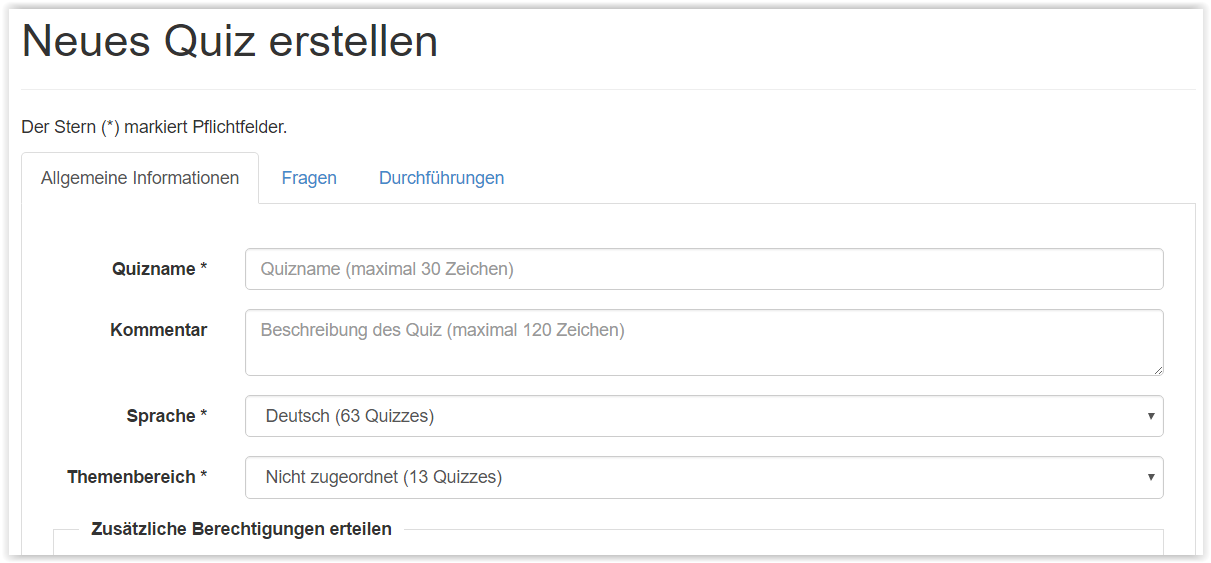
\includegraphics[width=0.8\textwidth]{Images/Quiz_Erstellen1.PNG}
	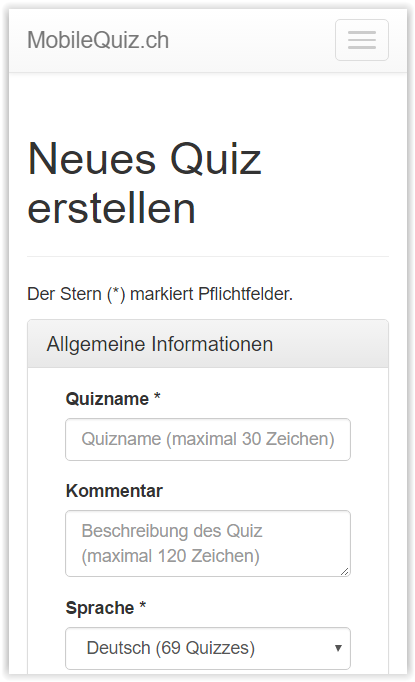
\includegraphics[width=0.3\textwidth]{Images/Quiz_Erstellen_Mobile.PNG}
	\caption{Desktop- und Mobile-Ansicht der Quiz-Erstellung}
\end{figure}

\bigskip
\textbf{Funktionale Umstellungen}
\bigskip

Da nun mit dem Quiz zusammen auch Fragen und Durchführungen erstellt werden, dauert dieser Vorgang länger als das alleinige Erfassen eines Quizzes in der bestehenden Mobile Quiz - Version. Da es sein kann, dass der Benutzer diesen Vorgang unterbrechen muss, beispielsweise arbeitet er im Zug und muss umsteigen, sollten die Benutzereingaben zwischendurch gespeichert werden.

Für die Umsetzung wäre ein halb-minütiger Countdown möglich gewesen, bei dessen Ablauf alle Daten im Hintergrund an den Server geschickt werden. Die Probleme liegen darin, dass der Ersteller im schlimmsten Fall 29 Sekunden Arbeit verliert oder unnötig viele Daten verschickt werden, falls keine oder nur wenige Änderungen vorliegen.

Aus diesem Grund wurde entschieden, jede neue Benutzereingabe einzeln an den Server zu senden. Dies wird mit \acrfull{AJAX} umgesetzt, welches es ermöglicht Daten an den Server zu schicken, ohne die gesamte Seite neu zu laden. Da jeweils nur ein Eingabefeld verändert wird, werden jeweils nur die wirklich benötigten Daten an den Server geschickt. Zudem ist die Handhabung auf dem Server ebenfalls einfacher, da meist nur ein Attributwert eines einzelnen Datenbank-Eintrages verändert werden muss.

Damit ein Benutzer weiss, dass seine Eingabedaten fortlaufend gespeichert werden, bekommt er jedes Mal eine entsprechende Meldung zurück. In Abbildung \ref{fig:Eingabe bei der Quiz-Erstellung} ist links ersichtlich, wie eine solche Meldung aussieht und rechts was der entsprechende \acrshort{AJAX}-Request an den Server beinhaltet.


\begin{figure}
	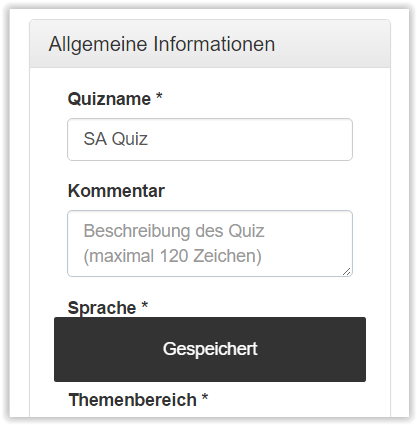
\includegraphics[width=0.35\textwidth]{Images/Quiz_Erstellen_Gespeichert.PNG}
	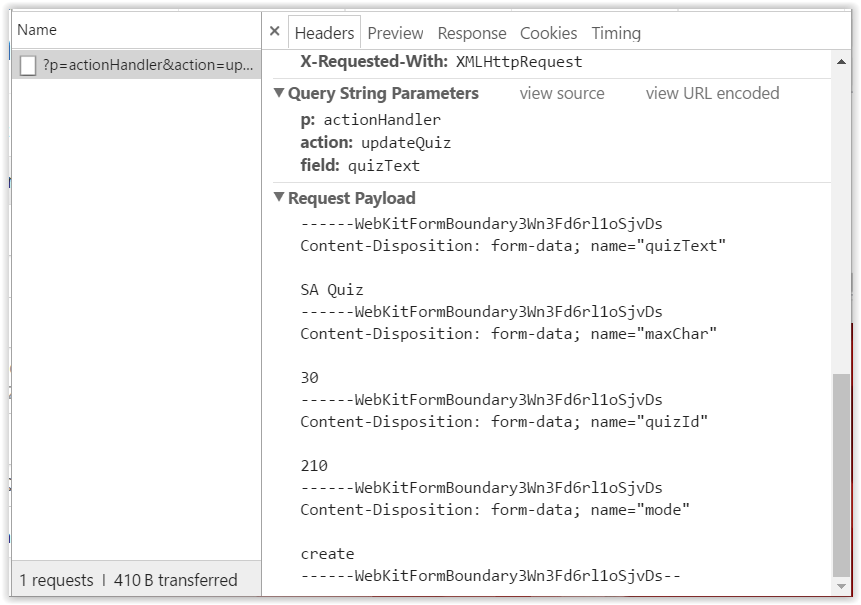
\includegraphics[width=0.65\textwidth]{Images/Quiz_Erstellen_Request.PNG}
	\caption{Eingabe bei der Quiz-Erstellung}
	\label{fig:Eingabe bei der Quiz-Erstellung}
\end{figure}

\bigskip\bigskip

\textbf{Frage-Erstellung}

\bigskip

Das oben beschriebene Design und die Kommunikation mit \acrshort{AJAX} wurde ebenfalls für die Frage-Erstellung umgesetzt. Dabei waren die Überlegungen die gleichen. \\

Zusätzlich wurde implementiert, dass eine Frage erst mit der ersten Benutzereingabe erstellt wird. Will sich ein Ersteller die Eingabemaske nur ansehen, so werden noch keine Daten in die Datenbank gespeichert.

Schliesslich wurde ein weiteres Verhalten implementiert, welches das Erfassen der Frage vereinfacht. Wenn ein Ersteller überprüfen will, ob seine Daten wirklich gespeichert wurden, so aktualisiert er die Seite und es wird normalerweise seine letzte angeforderte Seite erneut geladen. Dies ist in diesem Fall aber die Frage-Erstellungs-Seite, welche ihm ein neues, leeres Erfassungsformular anzeigt. Damit aber seine soeben eingegebenen Daten angezeigt werden, wurde mit JavaScript der \glqq Unload-Event\grqq abgefangen, welcher durch eine Seitenaktualisierung ausgelöst wird, und die angefragte \gls{URL} ausgetauscht, sodass neu die Frage-Bearbeitungs-Seite vom Server geladen wird.
Dieses Verhalten funktioniert bisher allerdings nur in Firefox \cite{firefox}.



\subsection{Umgestaltung Startseite Teilnehmer / Ersteller}

Die Startseite enthält neu nicht mehr die einzelnen Quizzes, sondern alle Durchführungen der Quizzes. Diese Umstellung war nötig, damit Teilnehmer ihre Durchführung leicht finden und nicht zuerst über das Quiz einsteigen müssen.

Wie im Abschnitt Interessensgruppen und Filterumstellung \ref{InteressensgruppenUndFilterumstellung} beschrieben, wurde ausserdem der Filter so angepasst, dass neu eine Mehrfachauswahl von Optionen möglich ist.

\bigskip\bigskip

\begin{quote}
	\glqq Probleme bereitete meist, dass Funktionen nicht auf den ersten Blick ersichtlich sind.\grqq
\end{quote}

Dies war eine der Schlussfolgerung des ersten \gls{Usability-Test}s und bezog sich vor allem auf die Startseite, da von dort aus die meisten Aktionen gestartet werden können. In dieser Arbeit wurde das Problem so angegangen, dass einerseits weniger Informationen zu den einzelnen Quizzes angezeigt werden und andererseits die Icons durch Text ergänzt wurden.

Konkret wurde die Anzahl Fragen, die Anzahl eigene Teilnahmen sowie die Anzahl Gesamtteilnahmen entfernt. Der Benutzer kann somit schneller die benötigten Informationen erfassen. Um die korrekte Durchführung zu finden war es jedoch nötig, zusätzlich den Durchführungstyp aufzuführen. 


\begin{figure}[H]
	\centering
	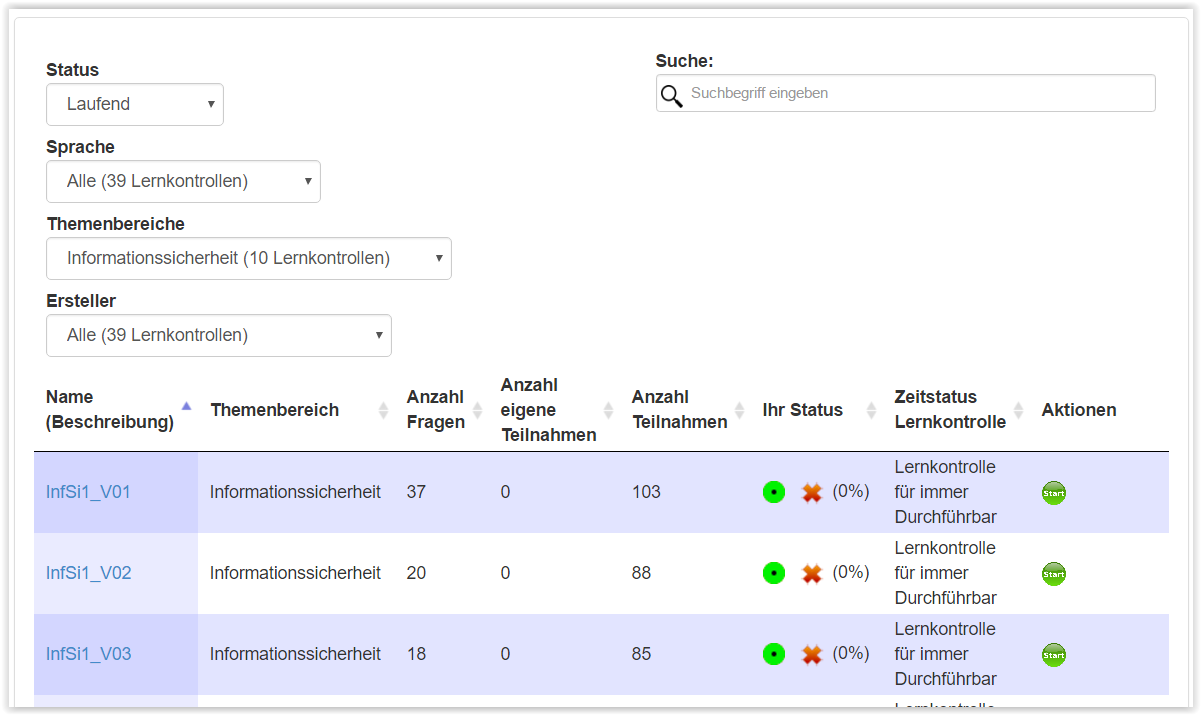
\includegraphics[width=0.8\textwidth]{Images/Startseite_alt.PNG}
	\caption{Startseite der bestehenden Mobile Quiz - Version 3}
	\cite{mobilequiz.ch}
\end{figure}


\begin{figure}[H]
	\centering
	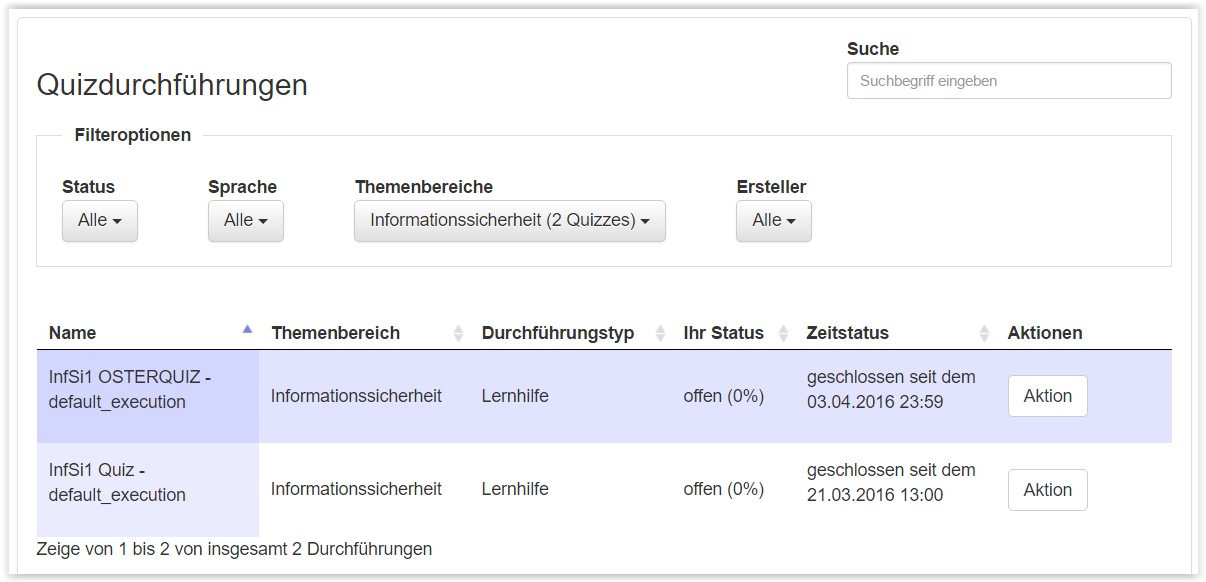
\includegraphics[width=0.8\textwidth]{Images/Startseite_neu.PNG}
	\caption{Neue Startseite für den Teilnehmer}
\end{figure}


Weiter wurden die unterschiedlichen Icons der Aktionen durch ein ausklappbares Menu ersetzt. Dieses beinhaltet die Aktionen als Text sowie einheitliche Icons. Dazu wurden Glyphicons von Bootstrap \cite{glyphicons} verwendet. Dies vereinfacht das Navigieren für den Benutzer, da er alle Aktionen beschrieben sieht und nicht, wie zuvor, erst mit der Maus über alle Symbole fahren muss. Dieses Verhalten war auf mobilen Geräten zudem gar nicht möglich, da es dort den \glqq Mouse-Hover-Effekt\grqq, also das darüberfahren mit der Maus, gar nicht gibt. Die neue Lösung ist somit auch mobile-tauglich.

Icons gibt es zwar weiterhin, diese dienen aber dem schnelle Erfassen der Auswahlmöglichkeiten und der Gruppierung von ähnlichen Aktionen.


\begin{figure}[H]
	\centering
	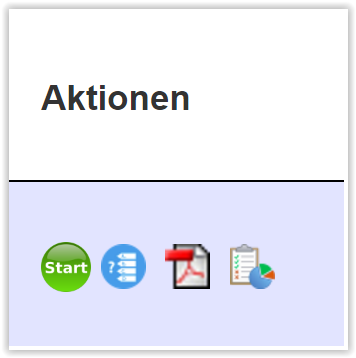
\includegraphics[width=0.3\textwidth]{Images/Aktionen_alt.PNG}
	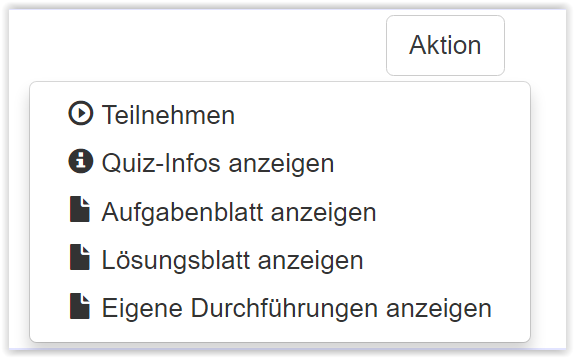
\includegraphics[width=0.5\textwidth]{Images/Aktionen_neu.PNG}
	\caption{Vergleich des bestehenden und der neuen Aktions-Anzeige}
	\cite{mobilequiz.ch}
\end{figure}







\section{Neuerungen}

\subsection{Fragen mit Bilder}

\subsubsection{Hochladen und Entfernen eines Bildes}
Bei jedem Fragetyp ist es neu möglich ein Bild zu hinterlegen. Die Funktion des Bild-Uploads auf den Server bestand bereits, wurde aber erweitert.
\\
\\
Beim Hochladen des Bildes wurde zuvor eine Fehlermeldung ausgegeben, wenn ein Bild eine Grösse von über 20 Megabyte überstieg. Diese Limite wurde herabgesetzt, weil ein Bild von dieser Grösse zu lange benötigt, bis es heruntergeladen werden kann. Unten ist ein Vergleich von Downloadzeiten bei verschiedenen Dateigrössen aufgeführt. Die angegebene Geschwindigkeit ist die Downloadgeschwindigkeit welche 80\% der Kunden erreichen. Diese wurden anhand von Speedtests der cnlab AG \cite{cnlab_speedtest} ermittelt. \\


\begin{tabular}{|c|c|c|c|}
	\hline 
	Dateigrösse & Art & Downloadgeschwindigkeit & Benötigte Zeit \\ 
	\hline 
	20 MB & DSL-Anbieter & 13,6 Mbit/s & 11,8 s \\ 
	\hline 
	20 MB & Kabel-Anbieter & 40,6 Mbit/s & 3,9 s \\ 
	\hline 
	20 MB & Mobile & 8,9 Mbit/s & 18 s \\ 
	\hline 
	5 MB & DSL-Anbieter & 13,6 Mbit/s & 2,9 s \\ 
	\hline 
	5 MB & Kabel-Anbieter & 40,6 Mbit/s & 1 s \\ 
	\hline 
	5 MB & Mobile & 8,9 Mbit/s & 4,5 s \\ 
	\hline 
	800 KB & DSL-Anbieter & 13,6 Mbit/s & 0,5 s \\ 
	\hline 
	800 KB & Kabel-Anbieter & 40,6 Mbit/s & 0,2 s \\ 
	\hline 
	800 KB & Mobile & 8,9 Mbit/s & 0,7 s \\ 
	\hline 
\end{tabular}\\

Falls ein Bild nun 800 Kilobyte übersteigt, so wird es so lange komprimiert, bis seine Dateigrösse darunterliegt. Dies wird durch die PHP-Funktion 'imagecopyresampled' erreicht. Als Code-Vorlage diente das Beispiel von www.williseiler.ch \cite{willis_php}. \\

Weiter gibt es Grössenbeschränkungen von Apache selbst \cite{stackoverflow_largeFilePHP}. Im File 'php.ini' können folgende drei Werte definiert werden:
\begin{itemize}
	\item upload\_max\_filesize: Legt die maximale Dateigrösse für eine Upload-Datei fest. Der Standardwert liegt bei 2 MB.
	\item post\_max\_size: Legt die maximale Grösse aller POST-Daten zusammen fest. Der Standardwert liegt bei 8 MB.
	\item max\_file\_uploads: Legt die maximale Anzahl aller Dateien fest, welche auf einmal hochgeladen werden können. Der Standardwert liegt bei 20 Dateien.
\end{itemize}

Werden via Excel-Template 10 Fragen mit je einem Bild à 1 Megabyte hochgeladen, so ist dies mit der Standardkonfiguration nicht möglich. Diese wurde deshalb folgendermassen angepasst:
\begin{itemize}
	\label{php.ini:neueGroessenbeschraenkungen}
	\item upload\_max\_filesize: Neu 5 MB. Grössere Dateien benötigen zu lange für den Upload. Allerdings soll der Benutzer nicht nur auf kleine Grössen beschränkt sein, deshalb wurde von der 2MB-Standardgrösse abgewichen.
	\item post\_max\_size: Neu 25 MB. Bei dieser Grösse beträgt die Uploadzeit bei einer Geschwindigkeit von 10,3 Mbit/s 19,4 Sekunden. Dies ist die Uploadgeschwindigkeit von 80\% der DSL-Messungen, welche beim Speedtest der cnlab AG \cite{cnlab_speedtest} erreicht wurde. Dem Benutzer sollte bewusst sein, dass der Upload bei so vielen Dateien einige Zeit in Anspruch nimmt.
	Auf der anderen Seite soll der Benutzer aber auch nicht eingeschränkt werden. Es soll möglich sein, gleichzeitig 20 Fragen mit Bildern à 1 MB sowie 1 Frage mit einem grösseren Bild plus das Excel-Template hochzuladen.
	\item max\_file\_uploads: Neu 25 Dateien. Der Standard-Wert wird nur leicht angehoben, da es möglich sein soll 20 Fragen mit Bildern gleichzeitig zu erstellen. Damit würde das Maximum von 20 Dateien nicht ausreichen.
\end{itemize}

Das Excel-Template für die Frage-Erstellung wurde ebenfalls erweitert, so dass auch Fragen mit Bilder erstellt werden können. Dazu wurde eine neue Spalte eingefügt, bei welcher man den Bildnamen inklusive Endung einträgt. Die Bilder müssen sich dabei im gleichen Ordner wie das Template befinden. Anschliessend wird der gesamte Ordner hochgeladen.

Es war dabei nicht möglich, nur die Excel-Datei alleine hochzuladen und anschliessend die Bilder selbstständig zu holen. Dies wäre bezüglich der Sicherheit höchst bedenklich.


\subsubsection{Anzeige eines Bildes}
Das Bild sollte beim Anzeigen der Frage gross genug dargestellt werden. Auf dem Computer war dies kein Problem, da ein Browserfenster genug Platz dazu bot, bei einem Smartphone hingegen war dieser beschränkt. Deshalb wurde die Anzeige so umgesetzt, dass das Bild beim Klick darauf auf dem ganzen Bildschirm dargestellt wird. Dies wurde mit Photoswipe \cite{photoswipe} umgesetzt, welches von GitHub \cite{github_photoswipe} bezogen wurde. Photoswipe ist eine JavaScript-Library, welche es ermöglicht, Bildgalerien auf Websites darzustellen. Sie unterstützt unter anderem Touch-Gesten und Zoom. So ist es kein Problem, ein Bild mit vielen Details darzustellen.

\begin{figure}
	\centering
	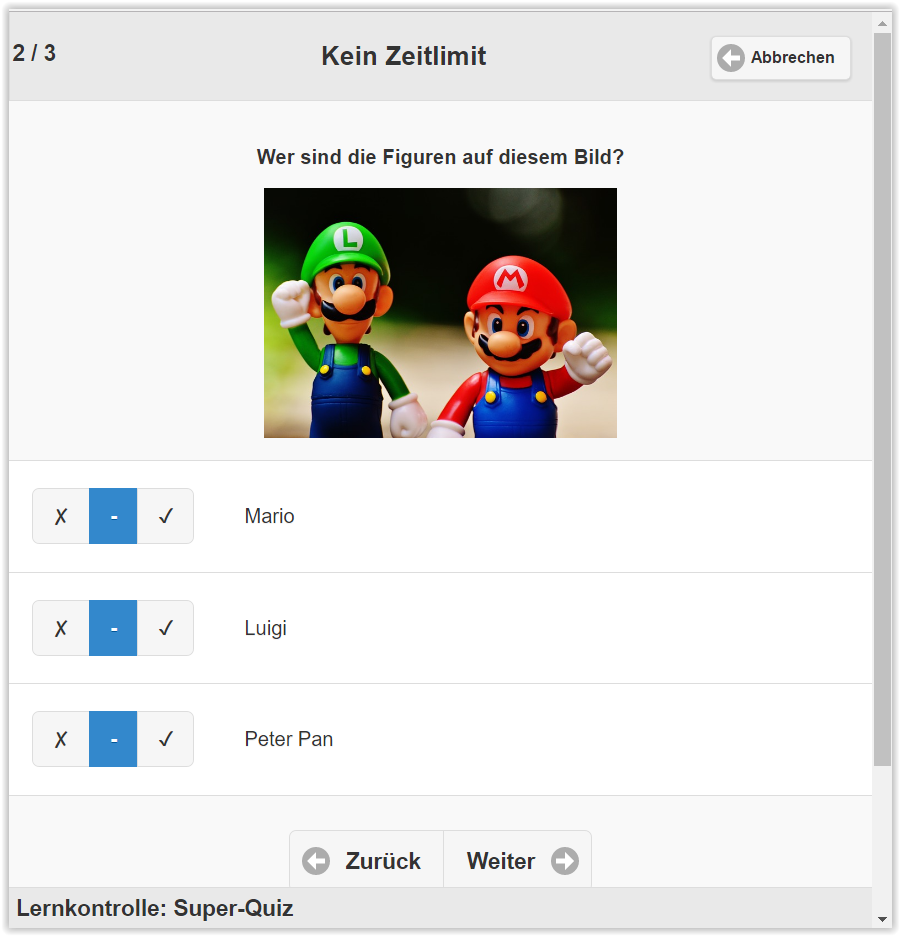
\includegraphics[width=0.5\textwidth]{Images/Frage-Bild_Anzeige_PC.PNG}
	\caption{Anzeige des Frage-Bildes am Computer}
	Quelle Fragebild: \cite{_bild_pixabay_mario_}
\end{figure}

\begin{figure}
	\centering
	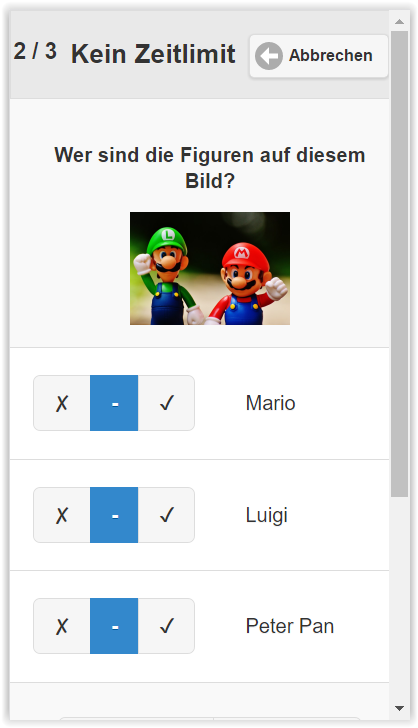
\includegraphics[width=0.3\textwidth]{Images/Frage-Bild_Anzeige_Mobile.PNG}
	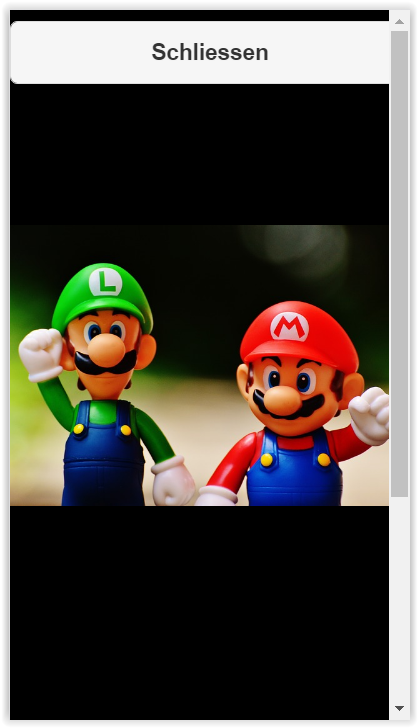
\includegraphics[width=0.3\textwidth]{Images/Frage-Bild_Anzeige_Mobile_Full.PNG}
	\caption{Anzeige des Frage-Bildes auf dem Smartphone}
	Quelle Fragebild: \cite{_bild_pixabay_mario_}
\end{figure}

Da sich eine Frage, bei welcher ein Bild hochgeladen wird, oft auf Inhalte aus dem Bild bezieht, wurde auch für die Auswertungsseite eine Bild-Anzeige implementiert. Somit können die Auswertungen besser nachvollzogen werden.

Weiter wurde die Generierung des PDF-Aufgabenblattes und Lösungsblattes ergänzt, damit auch dort die Bilder angezeigt werden. Hat man unterwegs kein Internet, so kann man sich die Fragen damit auch vorgängig herunterladen und im Zug anschauen.








\newpage
\subsection{Feedback an Quiz-Ersteller}
Bei der Ausarbeitung der neuen Fragetypen kam die Idee einer Freitext-Frage auf. Bei diesem Fragetyp sind keine Antwortmöglichkeiten vorgegeben, stattdessen schreibt der Teilnehmer seine Antworten in ein leeres Textfeld. Das Problem dabei ist aber die Korrektur, da eine korrekte Antwort auf viele verschiedene Wege niedergeschrieben werden kann. Aus diesem Grund wurde beschlossen, diesen Fragetyp nicht umzusetzen, aber die Idee andernorts zu verwenden.

Ist eine Frage unklar gestellt, gibt es Schreibfehler oder andere Verbesserungsmöglichkeiten, so musste dies ein Teilnehmer bis anhin selbst notieren und den Quiz-Ersteller, in den meisten Fällen der Dozent, im Unterricht fragen. Dies setzt aber voraus, dass der Quiz-Ersteller für den Teilnehmer immer ansprechbar ist. Erstellt ein Dozent aus Rapperswil ein Quiz, an welchem Teilnehmer der ganzen Schweiz mitmachen, so besteht diese Möglichkeit nicht.

Dieses Problem wurde nun angegangen. Unter jeder Frage gibt es neu die Möglichkeit einen Kommentar direkt an den Quiz-Ersteller zu senden.

\begin{figure}[H]
	\centering
	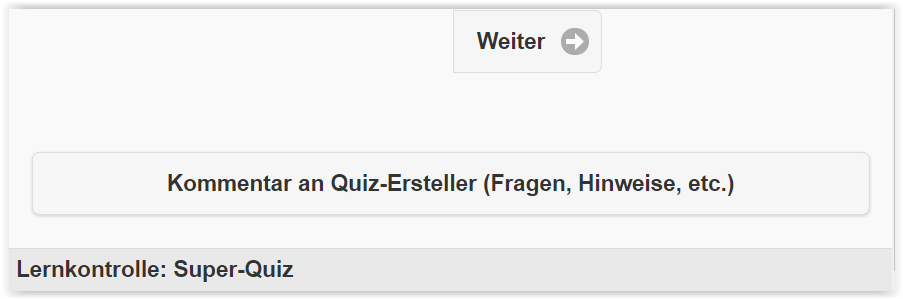
\includegraphics[width=0.7\textwidth]{Images/Feedback-Button.PNG}
	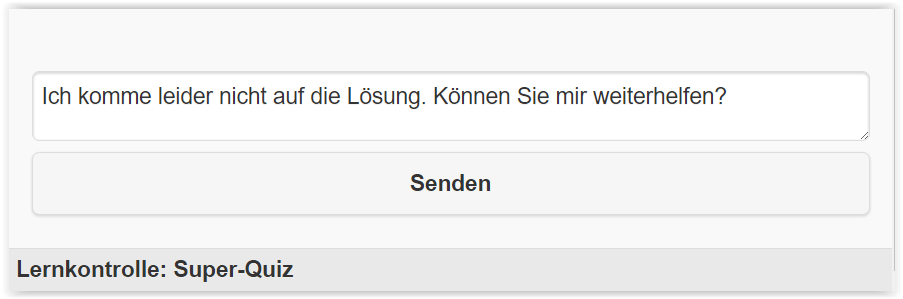
\includegraphics[width=0.7\textwidth]{Images/Feedback-Frage.PNG}
	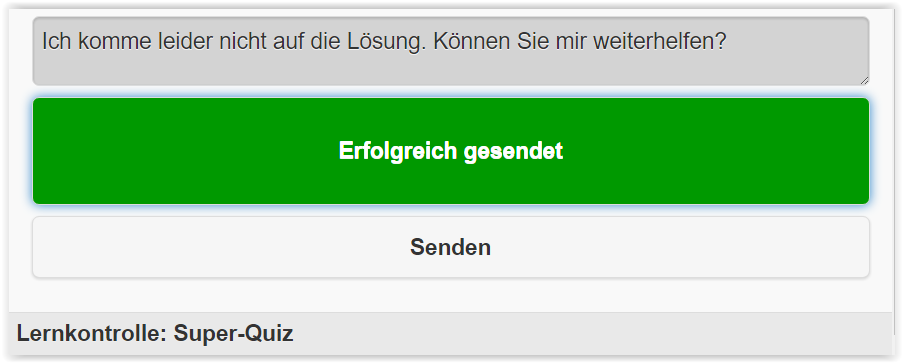
\includegraphics[width=0.7\textwidth]{Images/Feedback-Frage-gesendet.PNG}
	\caption{Ablauf der Feedback-Erfassung}
\end{figure}


Nach dem Senden des Feedbacks erhält der Quiz-Ersteller eine E-Mail. Darin ist nicht nur die Frage des Teilnehmers aufgeführt, sondern auch Informationen zum Teilnehmer selbst sowie die gesamte Frage inklusive Antwortmöglichkeiten. Somit hat der Quiz-Ersteller alle Informationen, um auf die Teilnehmer-Frage zu antworten.

\begin{figure}[H]
	\centering
	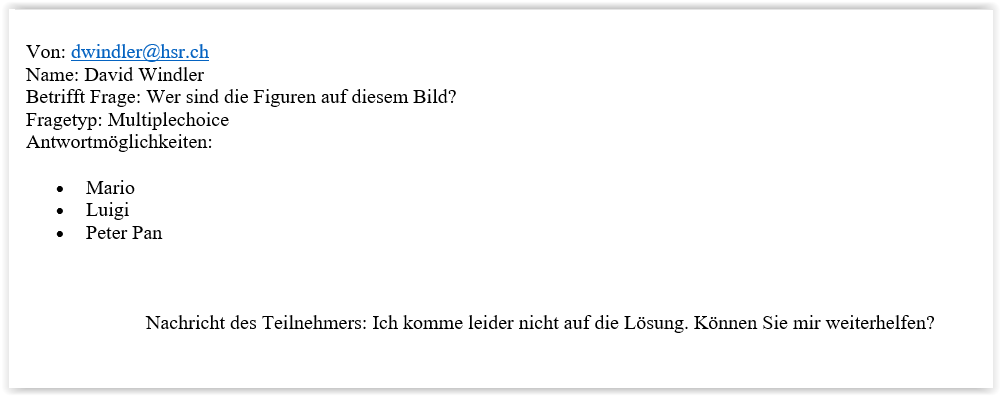
\includegraphics[width=0.9\textwidth]{Images/Feedback-Mail_Quiz-Ersteller.PNG}
	\caption{E-Mail an Quiz-Ersteller}
\end{figure}

Der Teilnehmer selbst erhält ein Bestätigungsmail mit den gleichen Informationen, wie sie auch der Quiz-Ersteller erhält.

\begin{figure}[H]
	\centering
	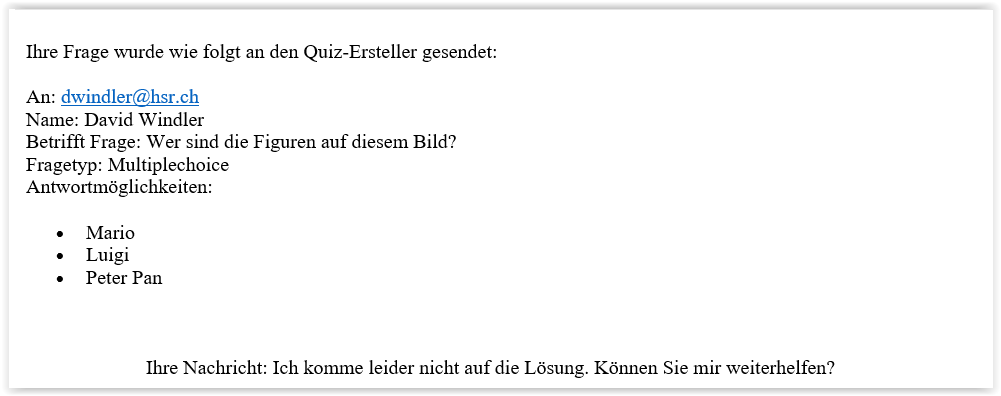
\includegraphics[width=0.9\textwidth]{Images/Feedback-Mail_Teilnehmer.PNG}
	\caption{Bestätigungs-E-Mail an Teilnehmer}
\end{figure}




\subsection{Interessensgruppen und Filterumstellung}
\label{InteressensgruppenUndFilterumstellung}
Loggt sich ein Teilnehmer bei Mobile Quiz ein, so soll er möglichst wenige Klicks von seinem zu lösenden Quiz entfernt sein. Dadurch spart er Zeit da, er sich nicht mit Filteroptionen und Suchfeldern auseinandersetzen muss. Doch wie erkennt Mobile Quiz welche Quizzes für den Teilnehmer interessant sind?

Möglich wäre es nachzuschauen, zu welchem Themengebiet der Teilnehmer schon Quizzes gelöst hat und aufgrund dessen die Filterauswahl bereits auf das Themengebiet mit seinen meisten Teilnahmen zu setzen. Das Problem dieser Methode liegt darin, dass sie für neu registrierte Teilnehmer nicht verwendet werden kann.
Aus diesem Grund wurde eine noch einfachere Methode implementiert. Dabei wird bei der Registrierung eines oder mehrere Interessengebiete angegeben. Diese werden dabei vorgemerkt und beim anschliessenden Aufruf aller Durchführungen wird der Themengebiet-Filter entsprechend der Interessensgebiete des Teilnehmers gesetzt. Meldet sich beispielsweise ein Student von \acrshort{CN1} bei Mobile Quiz an und setzt das Interessengebiet entsprechend, so werden zuerst immer die Quiz-Durchführungen von \acrshort{CN1} angezeigt. Besucht er zu einem späteren Semester das Modul Informationssicherheit 1, so kann er das Interessensgebiet jederzeit in seinen Profileinstellungen ändern.

\begin{figure}[H]
	\centering
	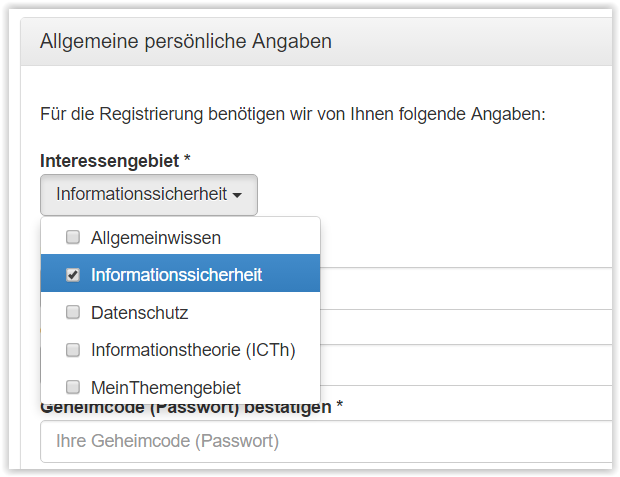
\includegraphics[width=0.5\textwidth]{Images/Themengebiet_Angabe_Registrierung.PNG}
	\caption{Angabe des Interessengebietes bei der Registrierung}
\end{figure}

Wie werden die Interessen der Teilnehmer in der Datenbank abgespeichert? Dazu half die Umstellung der Datenbank, welche es nun zulässt, dass ein Teilnehmer in mehreren Gruppen eingetragen werden kann.
Für jedes Themengebiet wurde eine Interessengruppe erstellt. Gibt ein Teilnehmer ein neues Interesse an, so wird er automatisch zur entsprechenden Interessen-Gruppe hinzugefügt. Interessengruppen werden automatisch mit der Erfassung eines neuen Themengebietes erstellt, beziehungsweise mit dem Entfernen wieder gelöscht und alle Teilnehmer ausgetragen.

\bigskip

Damit ein Teilnehmer mehrere Interessensgebiete angeben kann, war es nötig die Implementierung der Filter zu ändern. Bisher konnte jeweils nur eine Auswahl pro Filter gesetzt werden. Für die Umsetzung wurde die Library 'Bootstrap Multiselect' \cite{bootstrap_multiselect} von David Stutz verwendet. Durch eine Logikumstellung auf dem Server war es anschliessend für Quiz-Durchführungen und Fragen möglich eine Mehrfachauswahl pro Filter zu setzen.

\begin{figure}[H]
	\centering
	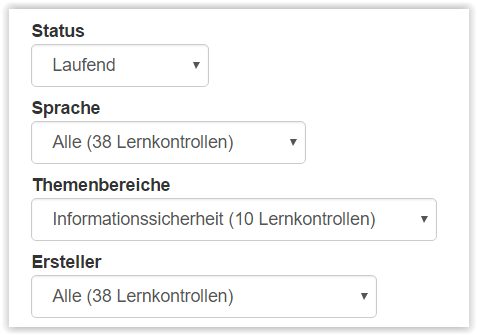
\includegraphics[width=0.462\textwidth]{Images/Alte_Filter_Mobile_Quiz.PNG}
	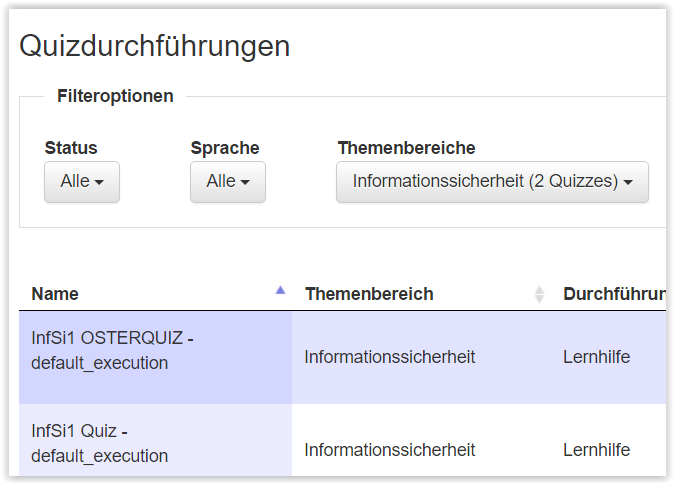
\includegraphics[width=0.45\textwidth]{Images/Neue_Filter_Mobile_Quiz.PNG}
	\caption{Filter der bestehenden (links) und der neuen (rechts) Mobile Quiz - Version}
	\cite{mobilequiz.ch}
\end{figure}



\newpage
\section{Schlussprodukt}

\begin{figure}[H]
	\centering
	\begin{itemize}
		\item Verbesserung der bestehenden Lösung
		\begin{itemize}
			\item \gls{Refactoring} und Fehlerbehebung
			\item Frage-Template
			\item Ablauf Quiz-Erstellung
			\item Design Quiz- und Frage-Erstellung
			\item Umgestaltung Startseite Teilnehmer/Ersteller
		\end{itemize}
		\item Neuerungen
		\begin{itemize}
			\item Fragen mit Bildern
			\item Feedback an Quiz-Ersteller
			\item Interessensgruppen und Filterumstellung
		\end{itemize}
	\end{itemize}
	\caption{Übersicht der Änderungen}
\end{figure}

Fasst man die Änderungen am bestehenden Mobile Quiz zusammen, so gab es einen überwiegenden Teil Überarbeitung der bestehenden Lösung sowie einen kleineren Teil von zusätzlichen Funktionalitäten. Die Verbesserungen kamen dabei zu einem Grossteil aus den Erkenntnissen der ersten \gls{Usability-Test}s, welche zu Beginn der Arbeit durchgeführt wurden. Diese sind im Anhang auf Seite \hyperlink{page.\getpagerefnumber{pdf:UTAW1}}{\getpagerefnumber{pdf:UTAW1}} zu finden. Die Wirkung davon blieb nicht aus, denn in der zweiten Durchführung gab es viel weniger Probleme mit dem Lösen der gegebenen Aufgaben, wie auf Seite \hyperlink{page.\getpagerefnumber{pdf:UTAW2}}{\getpagerefnumber{pdf:UTAW2}} ersichtlich ist.
Ausserdem haben die Fehlerbehebungen zu Beginn die Zuverlässigkeit von Mobile Quiz erhöht, was allen Benutzern zugute kommt und was das Vertrauen der Benutzer steigert.

Die Neuerungen ergänzen die Online Quiz-Plattform in verschiedenen Bereichen. Die Bild-Fragen geben dem Ersteller neue Möglichkeiten zur Wissensabholung und machen die Teilnahme an einem Quiz für Teilnehmer spannender.
Das Feedback an den Quiz-Ersteller erhöht die Kommunikation zwischen Teilnehmer und Quiz-Ersteller und soll dabei helfen Unklarheiten möglichst schnell aus dem Weg zu schaffen.
Schliesslich ist das Ziel der Interessensgruppen, dass Teilnehmer möglichst nur das sehen, was sie auch interessiert. Dadurch soll ein langes Suchen nach der gewünschten Quiz-Durchführung vermieden werden, wodurch die Bedienung als angenehm empfunden werden soll.

\bigskip

Alles in allem konnte Mobile Quiz durch die Umsetzung der oben beschriebenen Punkte zu einer verlässlicheren und bedienungsfreundlicheren Quiz-Plattform umgestaltet werden.



	
	\chapter{Inhalte für Folgearbeiten}
	% !TEX root = Projektdokumentation.tex

\newacronym{SE1}{SE1}{Software-Engineering 1}


\section{Arbeiten für die HSR}
\label{sec:ArbeitenFuerDieHSR}

\subsection{Nicht fertiggestellte Arbeiten}

\begin{itemize}
	\item Implementierung der Durchführung\\
	Damit ein Quiz wieder komplett erstellt werden kann, muss die Erstellung der Durchführung fertig implementiert werden. Für die Umsetzung ist einerseits die Datei \glqq createEditExecution \grqq für die Darstellung und Benutzerinteraktion, andererseits \glqq action\_execution\grqq für die Logik auf dem Server mit der Datenbankkommunikation wichtig. Was noch gemacht werden muss, ist die Abspeicherung der Daten im Tab Einstellungen und im Tab Publikation. Der Tab Allgemeine Informationen ist bereits vollständig umgesetzt und kann als Beispiel verwendet werden, um die noch notwendigen Implementierungsschritte zu erkennen. Der Tab Teilnehmer wurde ebenfalls vollständig umgesetzt.
	\item Erstellung aller Interessengruppen\\
	Ein Teilnehmer kann derzeit angeben für welche Themenbereiche er sich interessiert. Es wurde jedoch noch nicht zu allen bestehenden Themen eine entsprechende Interessengruppe in der Datenbank erstellt. Diese Datenbankbefehle müssen von Hand gemacht werden, da jede Gruppe ein eindeutiges Token benötigt. Ein Beispiel der Umsetzung ist nur für die Gruppe \glqq interest\_group\_Informationssicherheit\grqq vorhanden, welches in der Zusammenstellung aller Datenbank-Änderungen im Anhang vorhanden ist.
	Der Rest der Logik wurde komplett implementiert. Die Eintragung des Interesse am Themengebiet, das Setzen des Filters gemäss Interesse sowie das nachträgliche Verändern der Interessen funktionieren.
\end{itemize}



\subsection{Weiterentwicklung}

\begin{itemize}
	\item Fehlermeldung bei zu grossem Bild\\
	Wird ein Bild über 5 MB  hochgeladen, wird es von Apache nicht angenommen, da dies in der Datei \glqq php.ini\grqq so festgelegt wurde. Der Benutzer erhält nur einen allgemeinen Fehlercode. Das Übersteigen der Bildgrösse soll abgefangen und dem Benutzer ein spezifischer Fehlercode ausgegeben werden.

	\item Optimierung der Datenbank\\
	Allenfalls Änderung des Speichermodells, da beispielsweise das Abspeichern jeder eingegebenen Antwort in «an\_qu\_user» sehr viele Datenbankeinträge generiert.

	\item Aufräumen und Vereinheitlichung des Programm-Codes\\
	Es gibt einige Code-Stellen, welche gar nie aufgerufen werden, oder welche leserlicher geschrieben werden könnten. Zudem sind sehr viele verschiedene Programmierstile aufzufinden.

	\item Vereinheitlichung der Error-Codes\\
	Derzeit sind alle Error-Codes in der Datei \glqq errorCodeHandler.php\grqq abgelegt. Ein Code (-1) kann bei jeder Seite etwas komplett anderes bedeuten. Allenfalls könnten 3-Stellige Codes verwendet werden, bei denen alle 1XX für Datenbank-Fehler stehen, alle 2XX für Berechtigungs-Fehler, usw.

	\item Language-Support\\
	Der Language-Support ist mit 2 Language-Files etwas unhandlich. Allenfalls kann eine bessere Methode gefunden werden, um MobileQuiz leichter in verschiedenen Sprachen anzubieten.\\
	In \acrfull{SE1} wird für Java der Umgang mit Sprachfiles in Form von \glqq Resource Bundles\grqq vorgestellt, was ebenfalls eine Verwendung von mehreren Files pro Sprache ist, welche jeweils viele Key-Value-Paare beinhalten.
	
	\item Zurücksetzen des Filters\\
	Hat man beispielsweise beim Filter Themengebiete mehrere Werte ausgewählt und möchte nun alle Themengebiete anzeigen lassen, so müssen alle Werte einzeln abgewählt werden. Es soll bei allen Filtern eine zusätzliche Auswahlmöglichkeit \glqq alle\grqq vorhanden sein, um Filter schnell zurücksetzen zu können.
	
	\item Fehlermeldung bei offenem Request\\
	Falls für eine Frage noch eine offener Topic- oder Sprach-Request besteht, kann sie nicht gelöscht werden. Nach dem Klick auf das Lösch-Symbol bleibt die Frage in der Liste vorhanden, der Benutzer bekommt aber keine Rückmeldung warum. Er soll entsprechende Fehlermeldung angezeigt bekommen.
	
	\item Vergrösserung des Mobile-Menu\\
	Wählt man in der mobilen Version auf das Menu und anschliessend auf Profil, so ist nicht ersichtlich, dass ein Untermenu aufgeklappt wird. Der Grund liegt darin, dass dies in einem Bereich geschieht, welcher für den Benutzer nicht mehr sichtbar ist, da das Menu nicht gross genug angezeigt wird.
	
	\item Filteroption \glqq Alle\grqq \\
	Bei der eigenen Benutzung der neuen Filter fiel auf, dass es lange dauert, um mehrere ausgewählte Optionen abzuwählen, damit wieder alle Quizzes angezeigt werden. Allenfalls kann bei jedem Filter eine zusätzliche Single-Choice-Option \glqq Alle\grqq angeboten werden, um den entsprechenden Filter zurückzusetzen.
	
	\item Umsetzung der Verbesserungsvorschläge aus den zweiten Usability-Tests\\
	Da die zweite Durchführung der Usability-Tests erst in der letzten Projekt-Woche durchgeführt werden konnte, wurden die Ergebnisse daraus noch nicht umgesetzt. Sie sind im Anhang unter \glqq Auswertung Usability-Tests Durchführung 2\grqq zu finden.
\end{itemize}





\section{Inhalte für weitere Studentenarbeiten}
\label{sec:InhalteFuerStudentenarbeiten}

Während dieser Studienarbeit konnten nicht alle zusammengetragenen Arbeiten und theoretisch erarbeitete Konzepte umgesetzt werden. Alle möglichen Arbeiten sind im Anhang unter \glqq MoeglicheArbeitenSA\grqq zu finden, die Konzepte sowie deren Datenbankänderungen unter \glqq Konzept Gruppenmanagement\grqq, \glqq Konzept Neue Fragetypen\grqq und \glqq Konzept Statistiken\_Auswertungen\grqq.
		


\begin{itemize}
	\item Umgestaltung der Willkommensseite \\
	Wie im Kapitel \ref{subsec:Webuntersuchungen} beschrieben, besteht Verbesserungspotential beim ersten Eindruck von Mobile Quiz. Ein entsprechender Blog-Eintrag zu diesem Thema ist ebenfalls dort aufgeführt.
	
	\item Durchspielen vor Veröffentlichung \\
	Um ein Quiz auf Fehler zu Überprüfen soll es vor Veröffentlichung durchgespielt werden können. Dies ist bereits möglich, indem das Quiz auf privat gesetzt wird. Dies funktioniert aber nur im Administratoren-Modus korrekt.
	Wird das Quiz anschliessend veröffentlicht, soll der Ersteller gefragt werden, ob er die Quiz-Statistik zurücksetzen will. Ohne die Mitzählung seiner eigenen Teilnahme erhält er schlussendlich eine aussagekräftigere Auswertungsstatistik.
	
	\item Anonyme Teilnahme \\
	Ein Teilnehmer eines Quizzes soll sich nicht anmelden müssen. Eine Anonyme Teilnahme am Quiz soll möglich sein. Speziell daran ist die Handhabung von mehreren Sessions nicht erstellter Benutzer.\\
	Wird zudem ein privates Quiz erstellt, um es vor Veröffentlichung durchzuspielen, wird der Ersteller bei dessen Veröffentlichung gefragt, ob die Statistiken des Quizzes zurückgesetzt werden sollen. Somit wird sichergestellt, dass diese durch die Teilnahme des Erstellers nicht verfälscht werden.
	
	\item Sicheres Login und Passwort-Recovery
	Das Login sowie das Zurücksetzen des Passwortes sollen mittels OWASP Cheat-Sheets umgesetzt werden. Diese sind unter folgenden Links zu finden:
	\begin{itemize}
		\item Login \\
		\url{https://www.owasp.org/index.php/Authentication_Cheat_Sheet}
		\item Password-Recovery \\ \url{https://www.owasp.org/index.php/Forgot_Password_Cheat_Sheet}
	\end{itemize}
	
	\item Speicherung der Filter-Einstellungen \\
	Wählt der Benutzer eine Einstellung, ein Filter oder ähnliches, welches vom Standard-Fall abweicht, so soll dies in seinen Benutzerdaten gespeichert werden. In dieser Arbeit wurde bereits umgesetzt, dass der Teilnehmer ein oder mehrere Interessengebiete angeben konnte. Wechselte er auf die Ansicht aller Quizzes, so wurde zuerst nach diesen Interessengebieten gefiltert.
	
	
	\item Statistiken
	\begin{itemize}
		\item Statistiken pro Gruppe
		\item Statistiken über mehrere Quizzes \\
		Die Auswertungen sollen nicht nur für ein Quiz ersichtlich sein. Es soll auch möglich sein, mehrere Quizzes auszuwählen und sich von allen zusammen die Auswertung anzeigen zu lassen.
		\item Statistiken pro Gruppe über mehrere Quizzes \\
		Die Ergebnisse, welche eine Gruppe über mehrere Quizzes hinweg erreicht hat, sollen als Verlauf dargestellt werden. So kann P. Heinzmann prüfen, wie die CN1-Teilnehmer über das Semester hinweg die Lernhilfen der Vorlesung gelöst haben.
		\item Der Quiz-Ersteller soll bei einem Testat sehen, wer von der Gruppe das Testat bestanden hat und wer nicht. (z.B. Rot/Grün eingefärbt)
	\end{itemize}
	
	
	\item Mockups umsetzen \\
	\begin{itemize}
		\item Umsetzung der ausgearbeiteten Mockups\\
		Die in dieser Arbeit erstellten Mockups konnten nicht alle umgesetzt werden. Einige der im Anhang befindlichen Screens können deshalb noch umsetzt werden. Dabei sind die Hinweise im Kapitel \ref{chap:mockups} zu beachten.
		
		\item Erfassung von Gruppen \\
		In der Ansicht \glqq Quiz Erstellen – Administration\grqq soll die Möglichkeit bestehen, Gruppen zu erfassen. Wird ein Quiz anschliessend veröffentlicht, so wird diese Gruppe benachrichtigt.
		
		\item Anzeige von wichtigen Quizzes \\
		Ziel ist es, dass einer Gruppe ein Quiz, beispielsweise als Testat, zugewiesen werden kann. Anschliessend sieht der Teilnehmer auf der Quiz-Übersichts-Seite sofort, welche Quizzes seine sofortige Bearbeitung benötigen.
		Im Optimalfall sieht der Teilnehmer durch diese Option sowie durch das automatische Setzen des Filters nach seinen Interessen bereits alle Quizzes, welche er benötigt.
		
		\item Auswertungs-Darstellung \\
		Bei der Auswahl der Quiz-Einstellung «nur richtige Anzeigen» wird in der Auswertung bei den falsch beantworteten Fragen ein «?» anstatt die korrekte Antwort angezeigt. Dies verstehen die Studenten nicht. Überlegen, wie man dies besser darstellen kann.
		
		\item Ergänzung des Auswertungs-Screens\\
		In den Auswertungen für den Ersteller soll nebst den totalen Anzahl Stimmen einer Antwort auch der prozentuale Anteil angegeben sein. So kann direkt abgelesen werden, wie viele der Teilnehmer sich der Antwort enthalten haben, also «keine Antwort» angewählt haben.
	\end{itemize}
	
	\item Automatisch Erfassung von Teilnehmern und Gruppen \\
	Die Erfassung aller Teilnehmer für eine Vorlesung soll durch den Administrator erfolgen können. Dieser zu Beginn des Semesters alle Studenten via einer Excel-Datei ein, welche er von \url{www.unterricht.hsr.ch} generieren liess. Mobile Quiz erstellt automatisch die Teilnehmer. Auf einer Gruppen-Management-Seite weist der Administrator die Teilnehmern dann den Gruppen zu.
	
	\item Durchführungsbeschränkungen \\
	Es soll möglich sein zu unterscheiden, ob nur zugewiesene Gruppen ein Quiz durchführen können oder ob das Quiz allen offenstehen soll.
	
	\item Umsetzung von Polls \\
	Zur Umsetzung sind  grundlegende Abklärungen zu erarbeiten.
	Als Vorlage für die bestehende Lösung durch Patrick Eichler diente \glqq Straw Poll\grqq . \cite{straw_poll} Weitere Informationen zu diesem Thema sind unter folgendem Link erhältlich, welcher von Herr Markus Stolze und Herr Frank Koch zugeschickt wurde. \url{https://dl.dropboxusercontent.com/u/8905964/Breeze/FUM_Tilly_Polling_Tools.pdf}
	
	\item Session pro Benutzer \\
	Die Session soll pro Benutzer und nicht pro Gerät erstellt werden. Ist ein Benutzer am Computer angemeldet und meldet sich anschliessend auch auf dem Smartphone an, so soll die Computer-Session beendet werden.
	
	\item Schlagwörter \\
	
	\item Frage-Einreichung von Teilnehmer \\
	Es gibt eine neue Funktion, mit der Teilnehmer eigene Vorschläge für Fragen und Antworten an den Quiz-Ersteller senden können. Der Ersteller des Quizzes kann dann die Vorschläge annehmen, ablehnen oder anpassen.
	
	\item Ursprungsseite beim Melden von Fehlern feststellen \\
	Beim Beheben von Fehlern wäre es nützlich zu wissen, auf welcher Seite sich der Benutzer befand, bevor er auf auf «Fehler melden» klickte.
	
	\item Status-Konzept überarbeiten \\
	Konzept der Status soll dabei überarbeitet werden: Welche gibt es genau und was verursacht ein Status-Übergang?
	Bisherige Status: offen (0\%), in Bearbeitung(1-99\%), erledigt(100\%)
	
	\item Benachrichtigung der Interessengruppe\\
	Wird ein neues Quiz zu einem Themenbereich erstellt, sollen alle in der Interessengruppe eingetragenen Teilnehmer per E-Mail informiert werden. Vom Erhalt dieser Nachrichten können sie auch abmelden.
	
\end{itemize}



	
	
	\chapter{Qualitätsmanagement}
	% !TEX root = Projektdokumentation.tex

\newglossaryentry{Usability-Tests}{name={Usability-Tests},description={Probanden aus der Zielgruppe der Anwendung werden Aufgaben gestellt, welche sie mit der bestehenden Anwendung lösen sollen. Dabei wird untersucht, welcher Weg zur Lösung der Aufgabe eingeschlagen wird und wo dabei Probleme auftauchen.}}

\newacronym{CN1}{CN1}{Computernetze 1}

\newglossaryentry{Wireframes}{name={Wireframes},description={Die Visualisierung stellt die Seitenstruktur und Featureumsetzung sehr grob und schematisch dar. Der Wireframe wird in schwarz-weiss-grau angefertigt und gleicht dadurch einer Skizze oder Bleistiftzeichnung. Dieses Art der Visualisierung ist sehr schnell, einfach und günstig zu erstellen. Dazu genügt Papier und Bleistift oder eine entsprechende Wireframe-Software.}}

\newacronym{UI}{UI}{User Interface}

\newglossaryentry{User Interface}{name={User Interface},description={Unter einer Benutzeroberfläche oder Benutzerschnittstelle (UI) versteht man die Art und Weise, wie Befehle und Daten in den Computer eingegeben werden. Die Benutzeroberfläche ist die Schnittstelle zwischen Computer und Mensch. \cite{itWissen_benutzeroberflache}}}

%Qualitätsmanagement: Messungen, Tests, Usability Tests, Code Review usw. (mit vollständiger Beschreibung der Anordnungen und Rahmenbedingungen)

\section{Usability}
\label{sec:usability}
Im Internet gibt es zahlreiche Online-Quizzes, auch für das schulische Umfeld. Damit Mobile Quiz häufig und gerne genutzt wird, gibt es einige Faktoren zu beachten. \cite{marketingfire.de} Dazu zählen unter anderem das Design und die Strukturierung der Seite. \\

Wie gut die bestehende Mobile Quiz - Version in diesen Bereichen abschneidet, kann mit einem \gls{Usability-Tests} festgestellt werden. Davon wurden zwei Durchführungen gemacht, wobei die erste zu Beginn der Arbeit dabei half, Schwierigkeiten in der Bedienung offenzulegen. Anschliessend flossen die Ergebnisse draus in die Aufgabenstellung mit ein. Gegen Ende der Arbeit fand dann die zweite Durchführung statt, um zu messen, welche Fortschritte durch die Arbeit gelungen sind.

\subsection{Methoden}
Bei den \gls{Usability-Tests} zu Beginn der Arbeit nahmen drei Studenten der \acrfull{CN1}-Vorlesung, ein Student aus der Raumplanung sowie ein Student aus dem 5. Semester Informatik teil, was der Zielgruppe von Mobile Quiz entspricht. Zudem hatten die Studenten aus \acrshort{CN1} erst wenig Erfahrung damit gesammelt. \\
Bei der Durchführung wurden die Teilnehmern in Situationen hineinversetzt, welche bei der Benutzung von Mobile Quiz oft vorkommen (siehe Usability-Test\_Aufgabenstellung). Die Teilnehmer wurden dabei eins zu eins beobachtet und Schwierigkeiten oder Abweichungen von den Erwartungen (siehe Usability-Test\_Erwartungen) notiert. Die Gesamtauswertung wurde anschliessend in einem separaten Dokument festgehalten (siehe Usability-Test\_Auswertung). Die erwähnten Dokumente befinden sich im Anhang.

\subsection{Erkenntnisse}
% Hier folgen sämtliche Erkenntnisse zum Bereich Usability.
% Auch die Auswertung was neu gemacht wird, kommt hier hin bzw. sicher eine Zusammenfassung und ganzes ist dann im Anhang.
Die Durchführung der \gls{Usability-Tests} zeigte, dass vor allem im Bereich der Benutzerführung Probleme vorhanden sind, denn die vorhandenen Funktionen werden nicht auf den ersten Blick gefunden.
Aus den Erkenntnissen der \gls{Usability-Tests} sowie den eigenen Tests mit dem MobileQuiz wurden die ersten \gls{Wireframes} erstellt, diese befinden sich im Anhang. 

\section{Codestatistik}
Mit Codestatistiken soll erkannt werden, ob sich die Codequalität während der Arbeit verbessert oder nicht. Dafür wird das Webtool Code Climate eingesetzt.

Der nachfolgende Screenshot zeigt den Stand der Codequalität ganz zu beginn des Projektes. Die bereits eingezeichneten Verbesserungen sind entstanden, da die Grundeinstellungen auf unsere Bedürfnisse angepasst und verfeinert wurden.

\begin{figure}[H]
	\centering
	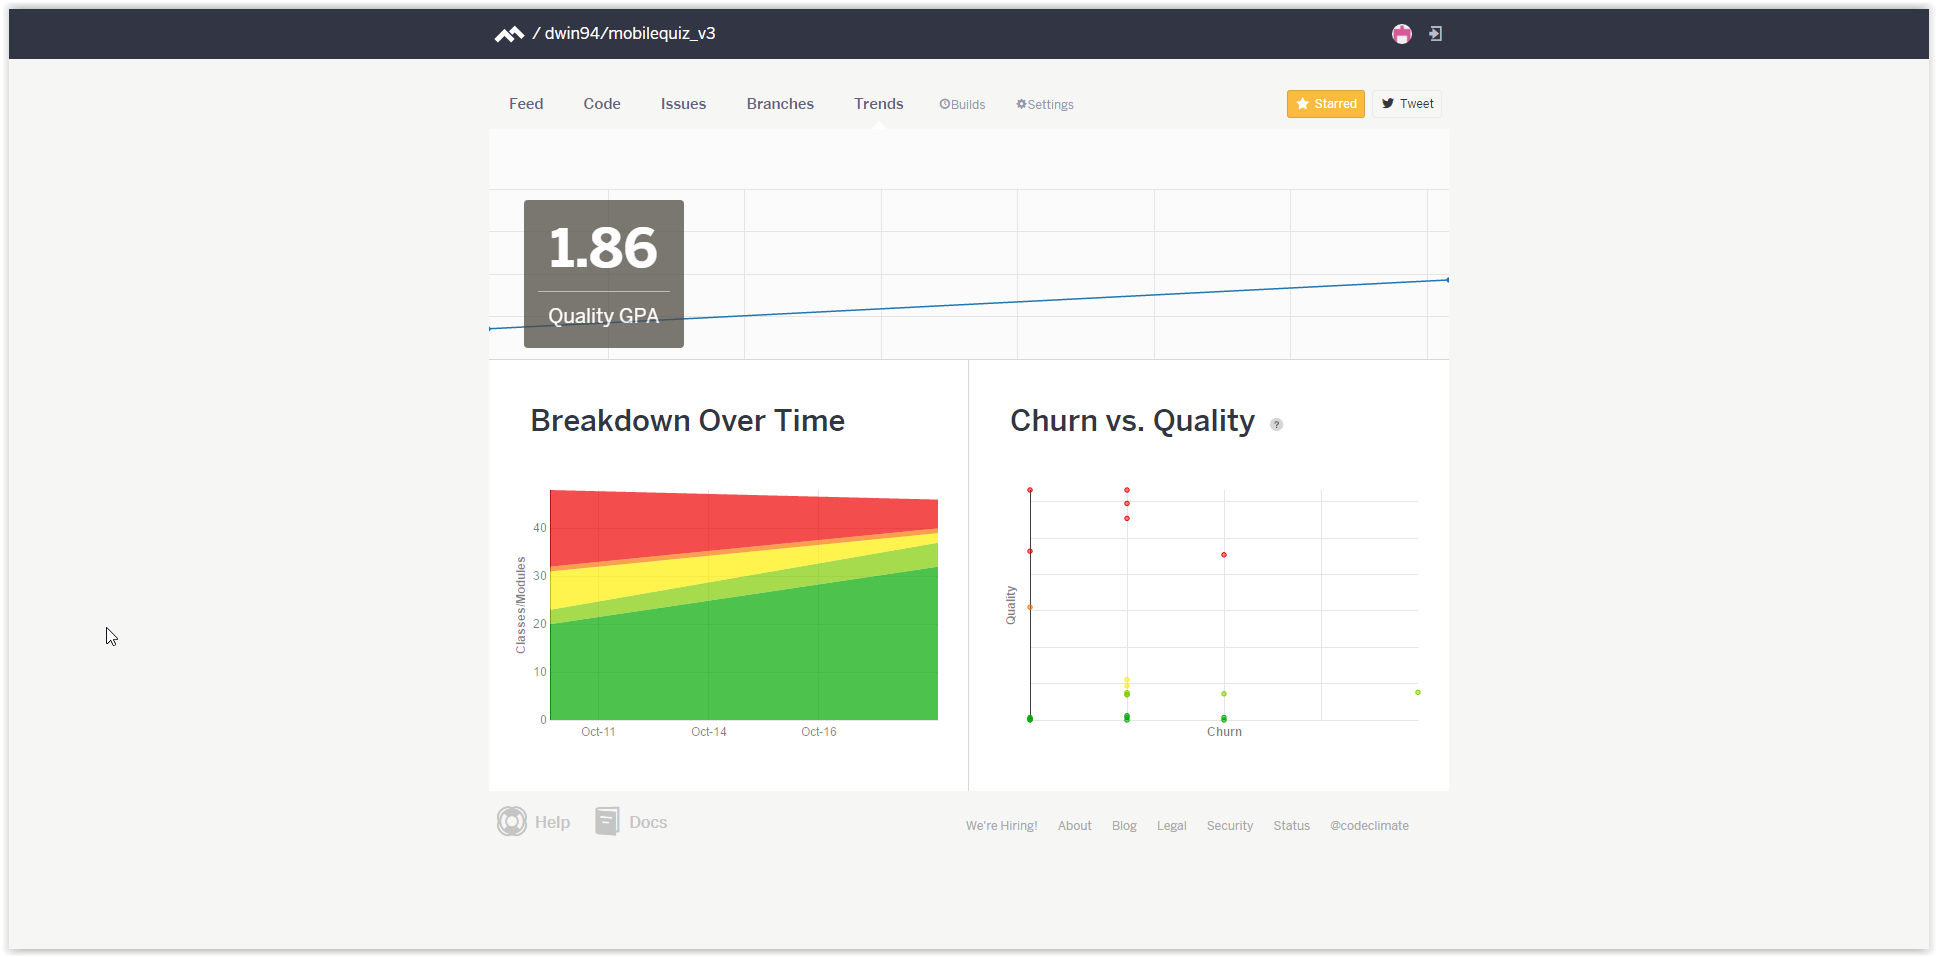
\includegraphics[width=1\textwidth
	]{Images/Stand_Beginn_181016.PNG}
	\caption{Code Climate Stand 18.10.2016 - nach der Verfeinerung der Regeln}
\end{figure}


\section{Systemtests mit Selenium}
%automatisierte Systemtests mit Selenium
Selenium IDE ist ein Firefox AddOn für Web-\acrfull{UI}-Tests. Es ermöglicht das Aufnehmen, die Bearbeitung, das Debuggen und das Abspielen von Tests. 

Mit der Hilfe dieses Tools können einfach \gls{User Interface} Tests durchgeführt werden.

\subsection{Methoden}
%Konkretes Vorgehen beschreiben
Mit dem Firefox Plugin von Selenium können die Abläufe die getestet werden sollen einfach aufgenommen werden. Das heisst der Benutzer spielt den korrekten Ablauf durch. Das einzige was von Hand gemacht werden muss, ist das assert-Statement, also die Prüfung, ob der Test korrekt durchgelaufen ist.

Alle erfassten Tests werden abgespeichert und können danach einfach abgespielt werden.

\subsection{Erkenntnisse}
%Was haben wir mit Hilfe von (siehe Titel) herausgefunden und wie werden wir es verbessern?
%Folgen sobald das Tool konkret eingesetzt wurde

\section{Code Review}
%Code Review mit GitHub Branch
%Einleitung
Mit einem Code Review wird die Codequalität sichergestellt. Dabei schaut sich jeweils derjenige, welcher den Code nicht geschrieben, den Code des anderen an. 


\subsection{Methoden}
%Konkretes Vorgehen beschreiben
Die Code Reviews wurden mit Github Branches gemacht. Das heisst der Entwickler eröffnet für seine neuen Features ein Github Branch und bevor dieser wieder in den Master merged werden kann, schaut sich das andere Teammitglied den Branch an und gibt in frei.

\subsection{Erkenntnisse}
%Was haben wir mit Hilfe von (siehe Titel) herausgefunden und wie werden wir es verbessern?
%Folgen sobald konkret eingesetzt wurde

\section{Unit-Tests}
%Unit-Tests mit PHPUnit
%Einleitung
Die Unit-Tests sind dazu da, einzelne Funktionen zu testen. Wenn eine Basis von Unit-Test bestehen, welche die Funktionalität des Codes abdecken, kann gut Refactoring betrieben werden. 

\subsection{Methoden}
%Konkretes Vorgehen beschreiben
Das Testen wurde mit PHPUnit umgesetzt. Diese Test werden bei jedem commit automatisch vom Continuous Integration Server, in unserem Fall Travis CI, ausgeführt. So wird bei jedem commit geschaut, ob noch alles funktioniert

\subsection{Erkenntnisse}
%Was haben wir mit Hilfe von (siehe Titel) herausgefunden und wie werden wir es verbessern?
%Folgen sobald konkret eingesetzt wurde



	
	
	
	
	\chapter{Literaturverzeichnis}
	%Im Literaturverzeichnis sind alle verwendeten Quellen (Bücher, Publikationen, Application Notes, Links (url), sowie Hinweise auf Gespräche mit bestimmten Personen) aufgeführt. Typischerweise werden die Quellenangaben nummeriert (z.B. [1], [2]) und in der Reihenfolge geordnet, wie sie im Bericht vorkommen. Man kann die Quellen auch mit den (abgekürzten) Namen der Autoren und dem Erscheinungsjahr bezeichnen (z.B. [Schueli90], [Shannon49]), wobei die Einträge dann alphabetisch geordnet werden. Jede Referenz ist so anzugeben, dass sie einfach auffindbar ist (evtl. inklusive Seitenzahl, Bibliothek Bestellnummer). Eine Referenz, welche die allgemeine Grundlage für ein ganzes Kapitel bildet, wird im Titel bzw. in einer Fussnote aufgeführt. Für Referenzen aus dem Internet soll ein kommentierter URL angegeben werden.
	\patchcmd{\thebibliography}{\chapter*}{\section*}{}{}
	\renewcommand{\bibname}{}
	\bibliographystyle{IEEEtran}
	\bibliography{zotero}
	
	
	\chapter{Abkürzungsverzeichnis (Glossar)}
	%Das Abhkürzungsverzeichnis (Glossar) enthält alle im Bericht vorkommenden Abkürzungen in alphabetischer Reihenfolge. Häufig wird hier auch eine Kurzbeschreibung zu den Begriffen angegeben. In diesem Fall nennt man den Abschnitt eher "Glossar".
	\renewcommand{\glossarysection}[2][]{}
	\printglossaries
	
	
	\chapter{Abbildungsverzeichnis}
	\renewcommand{\listfigurename}{}
	\listoffigures
	
	
	\part{Anhang}
	%Der Anhang enthält Abschnitte, welche den Rahmen oder die Kontinuität der Hauptkapitel stören, da sie nicht von zentraler Bedeutung für die Endlösung sind. Auch administrative Teile der Arbeit, welche von der Schule gefordert, für das Verständnis des Endergebnisses der Arbeit weniger wichtig sind, sollen im Anhang aufgeführt sein. Die im folgenden hervorgehobenen Punkte müssen in jeder Arbeit enthalten sein, die übrigen Punkte können je nach Situation vorkommen oder nicht.
	
	
	\chapter{Persönliche Berichte zur Arbeit}
	%Persönliche Berichte zur Arbeit (wie von HSR verlangt)
	\section{Persönlicher Bericht von Andrea Hauser}
	% !TEX root = Projektdokumentation.tex

Da wir das Thema unserer Studienarbeit auf eigenen Wunsch mit einbringen konnten, habe ich mich schon vor dem Semesterbeginn sehr darauf gefreut, diese Arbeit anzupacken. Dementsprechend hoch war auch die Motivation, die Studienarbeit anzugehen. Mit voller Überzeugung kann ich sagen, dass die Freude und die Motivation durchgehend bestehen geblieben sind. 

\bigskip

Die vierzehn Wochen, in welchen diese Studienarbeit bearbeitet wurde, sind wie im Flug vergangen. Dies lag sicher auch daran, dass wir mit insgesamt 36 ECTS einen gut gefüllten Stundenplan und sehr viele Abgaben hatten.
Auch wenn es teilweise stressige Zeiten gab und ich dann zum Schluss mit meinem Implementierungsteil nicht mehr ganz fertig geworden bin, kann ich sagen, dass ich mit dem Schlussresultat unserer Arbeit zufrieden bin.

\bigskip

Ich habe das Gefühl, dass ich anhand dieser Arbeit sehr viel mehr lernen konnte, als wenn ich das ganze nur in der Theorie angeschaut hätte. Ich hatte vorher noch nie in PHP programmiert und auch den ganze Umgang mit Servern kannte ich vorher noch nicht. Auch wenn ich bei der Zeiteinschätzung der Arbeitspakete manchmal stark daneben lag, hilft mir dies, in meinen in Zukunft anfallende Arbeiten realistischere Zeitschätzungen zu erhalten. Ich bin froh, dass ich diese Erfahrungen bereits hier im Studium sammeln konnte.

\bigskip
Zusammenfassend kann ich sagen, dass ich von dieser Studienarbeit nur profitieren konnte. Ich habe neben dem Engineering Projekt nun ein weiteres Projekt erfolgreich durchführen können und hoffe, dass ich für die Zeiteinschätzung weiter hinzugelernt habe.

	\newpage
	\section{Persönlicher Bericht von David Windler}
	% !TEX root = Projektdokumentation.tex

Die Studienarbeit ist mein zweites grosses Informatik-Projekt im Studium und auch in meiner bisherigen Laufbahn. Da ich zuvor eine KV-Lehre absolvierte und als Quereinsteiger ins Informatik-Studium startete fehlte mir vor allem die Praxiserfahrung. Trotz noch so vielem Lernaufwand konnte diese nie weggemacht werden. Aus diesem Grund bin ich sehr froh um die drei Praktischen Projekte während des Studiums - das Engineering-Projekt, die Studienarbeit und die Bachelorarbeit. Durch diese lerne ich den theoretisch erlernten Stoff des Studiums praktisch umzusetzen und Wissenslücken selbstständig zu schliessen.

\bigskip

Zu Beginn dieser Arbeit hatte ich mit vielen der eingesetzten Technologien von Mobile Quiz noch nie gearbeitet und sehr grossen Respekt davor. Kann ich wirklich selbst einen Apache-Server aufsetzen? Wie bekomme ich die Webseite auf den Server? Alles Fragen, welche ein Informatik-Lernender leicht hätte beantworten können, ich jedoch nicht wusste.
Diese und viele weitere Fragen beschäftigten mich, bis Andrea und ich, mit grosser Unterstützung von Patrick Eichler, Apache auf einer Server-Instanz der HSR zum laufen brachten. Von da an wusste ich, dass auch die restlichen Technologien mit genügend Ehrgeiz zu erlernen sind. Dies bewahrheitete sich auch, denn das Erlernen PHP und Latex bereiteten keine Mühe und auch die SQL-Kenntnisse aus dem ersten Semester konnten schnell wieder in Erinnerung gerufen werden.

\bigskip

Während des Projektes war ich vom vielen Recherche- und Schreibaufwand überrascht und freute mich deshalb umso mehr auf das Implementieren der erarbeiteten Konzepte. Diese Phase fiel jedoch mit vielen Abgaben von anderen Modulen zusammen, wodurch sich die Stunden am Computer anhäuften. Trotzdem machte es viel Spass zu sehen, wie schnell man neue Programmiersprachen lernt, wenn man sie nur oft genug verwendet.

\bigskip

Kurz zusammengefasst: Eine intensive, aber sehr spannende und lehrreiche Zeit.
	
	
	\chapter{Details zur Lösungsfindung}
	%Details zur Lösungsfindung (z.B. Analyseschritte, Designschritte, umfangreiche Herleitungen, Tabellen, Messergebnisse, Testauswertungen)
	
	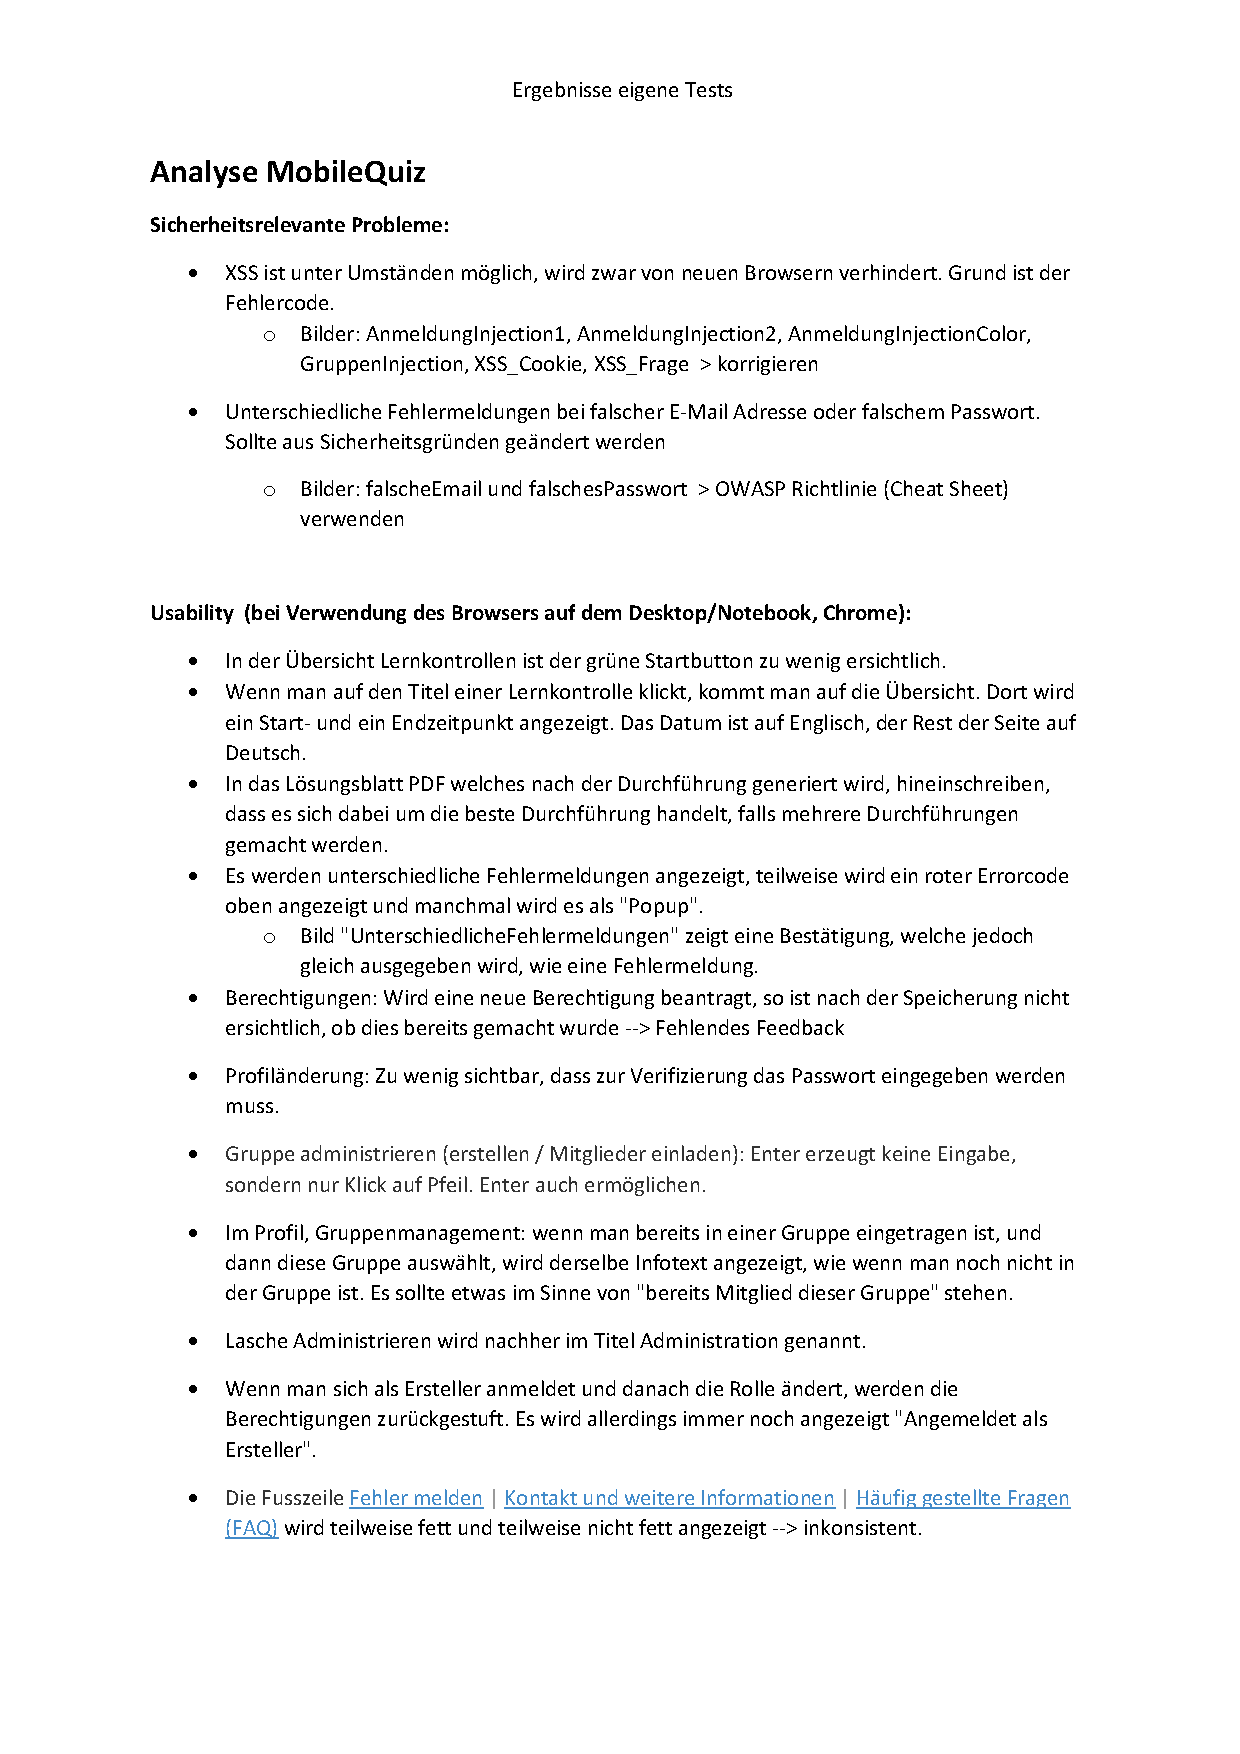
\includepdf[pages={1-5}, pagecommand={}]{PDFs/Ergebnisse_eigene_Tests.pdf}
	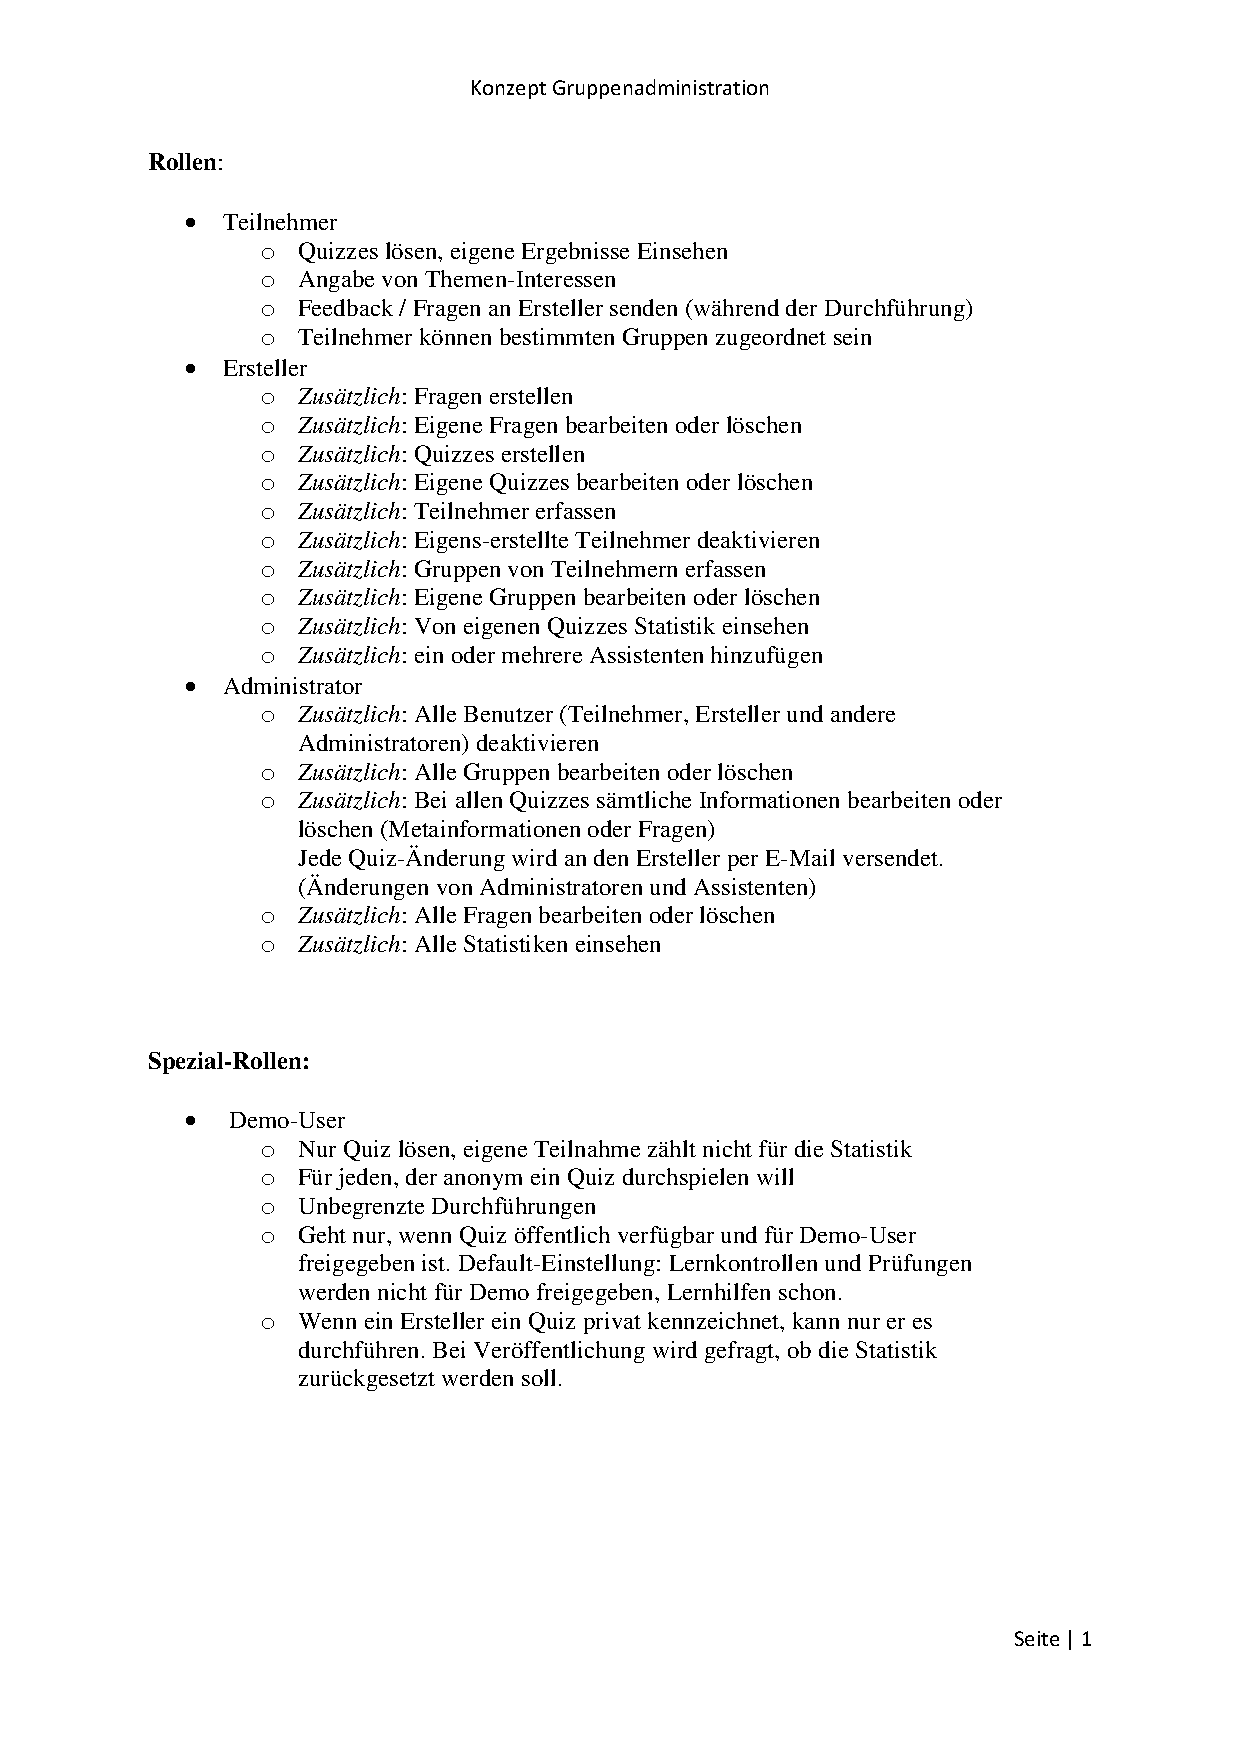
\includepdf[pages={1-6}, pagecommand={}]{PDFs/Gruppenadministration.pdf}
	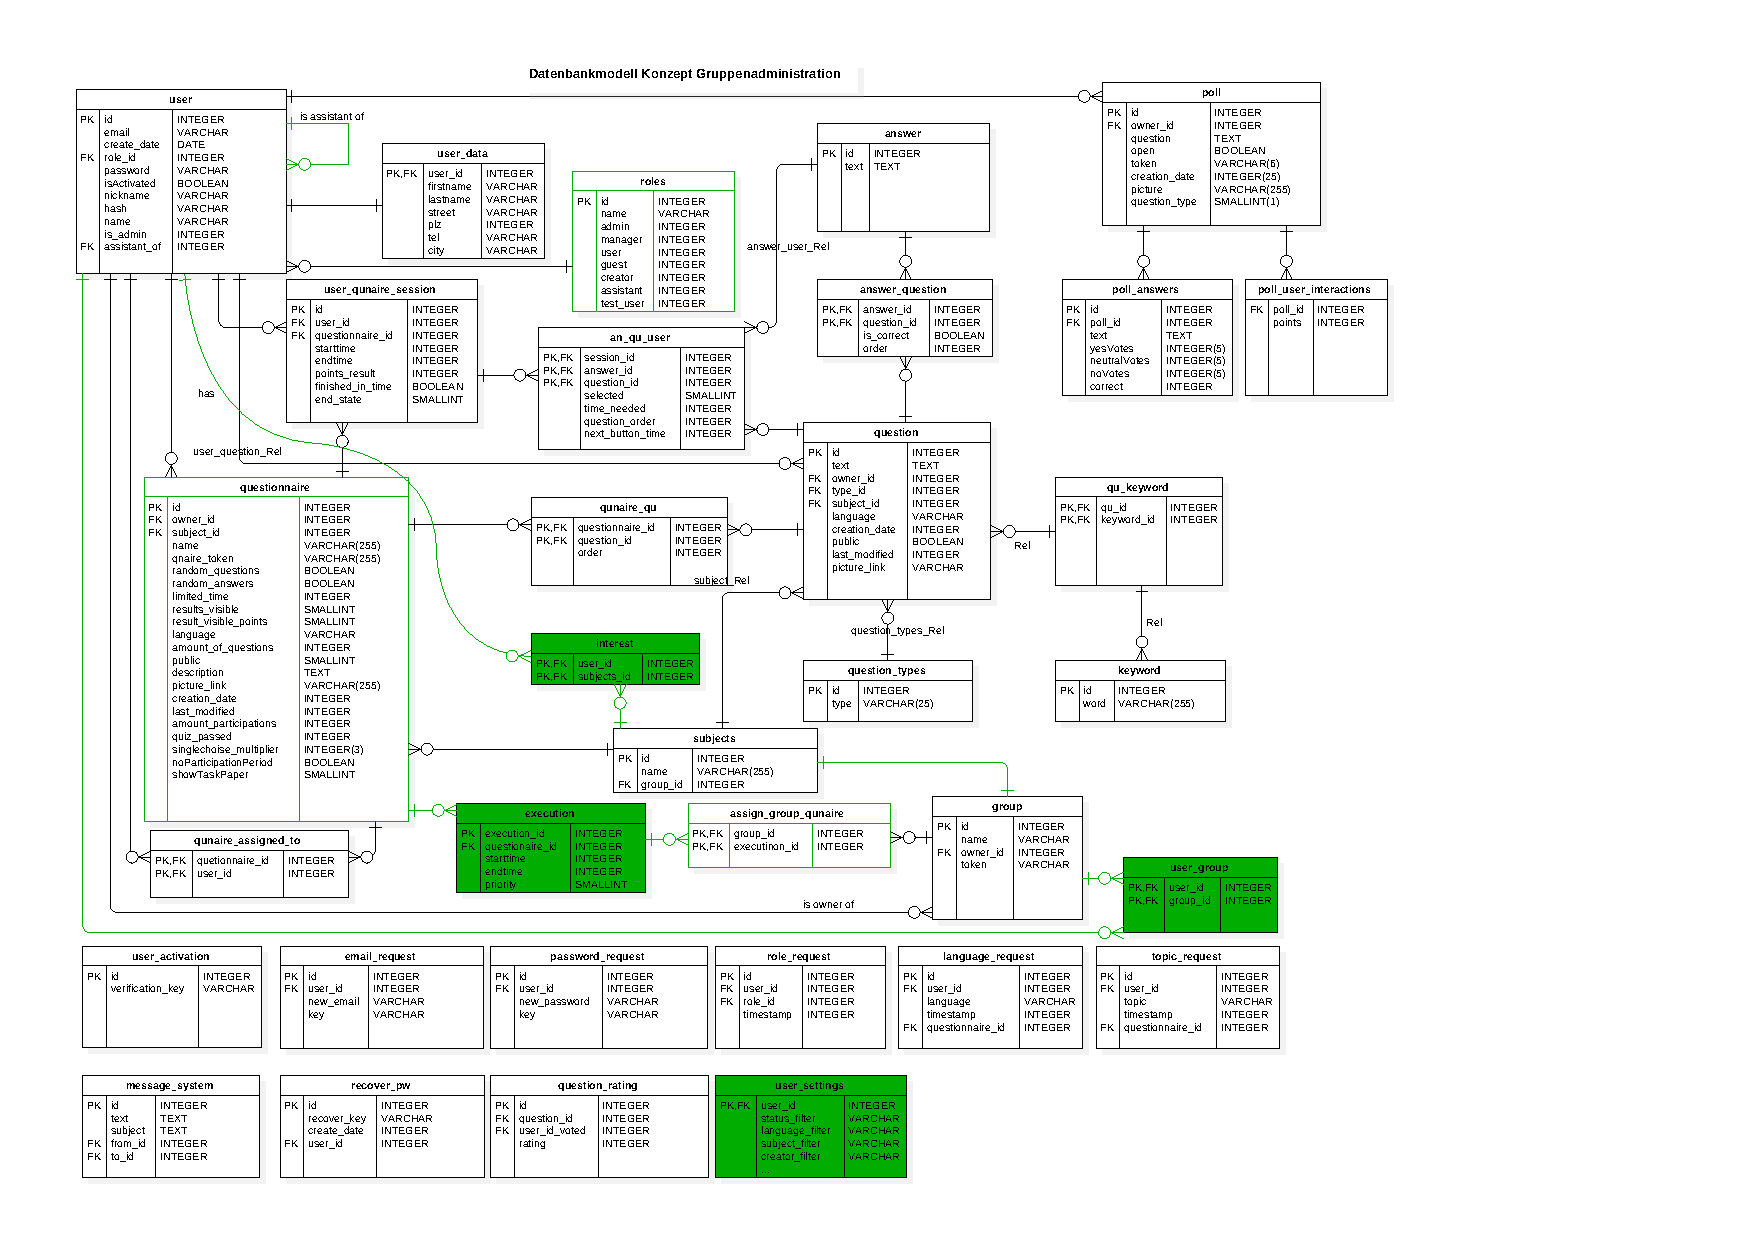
\includepdf[landscape=true, pagecommand={}]{PDFs/Gruppenadministration_DB.pdf}
	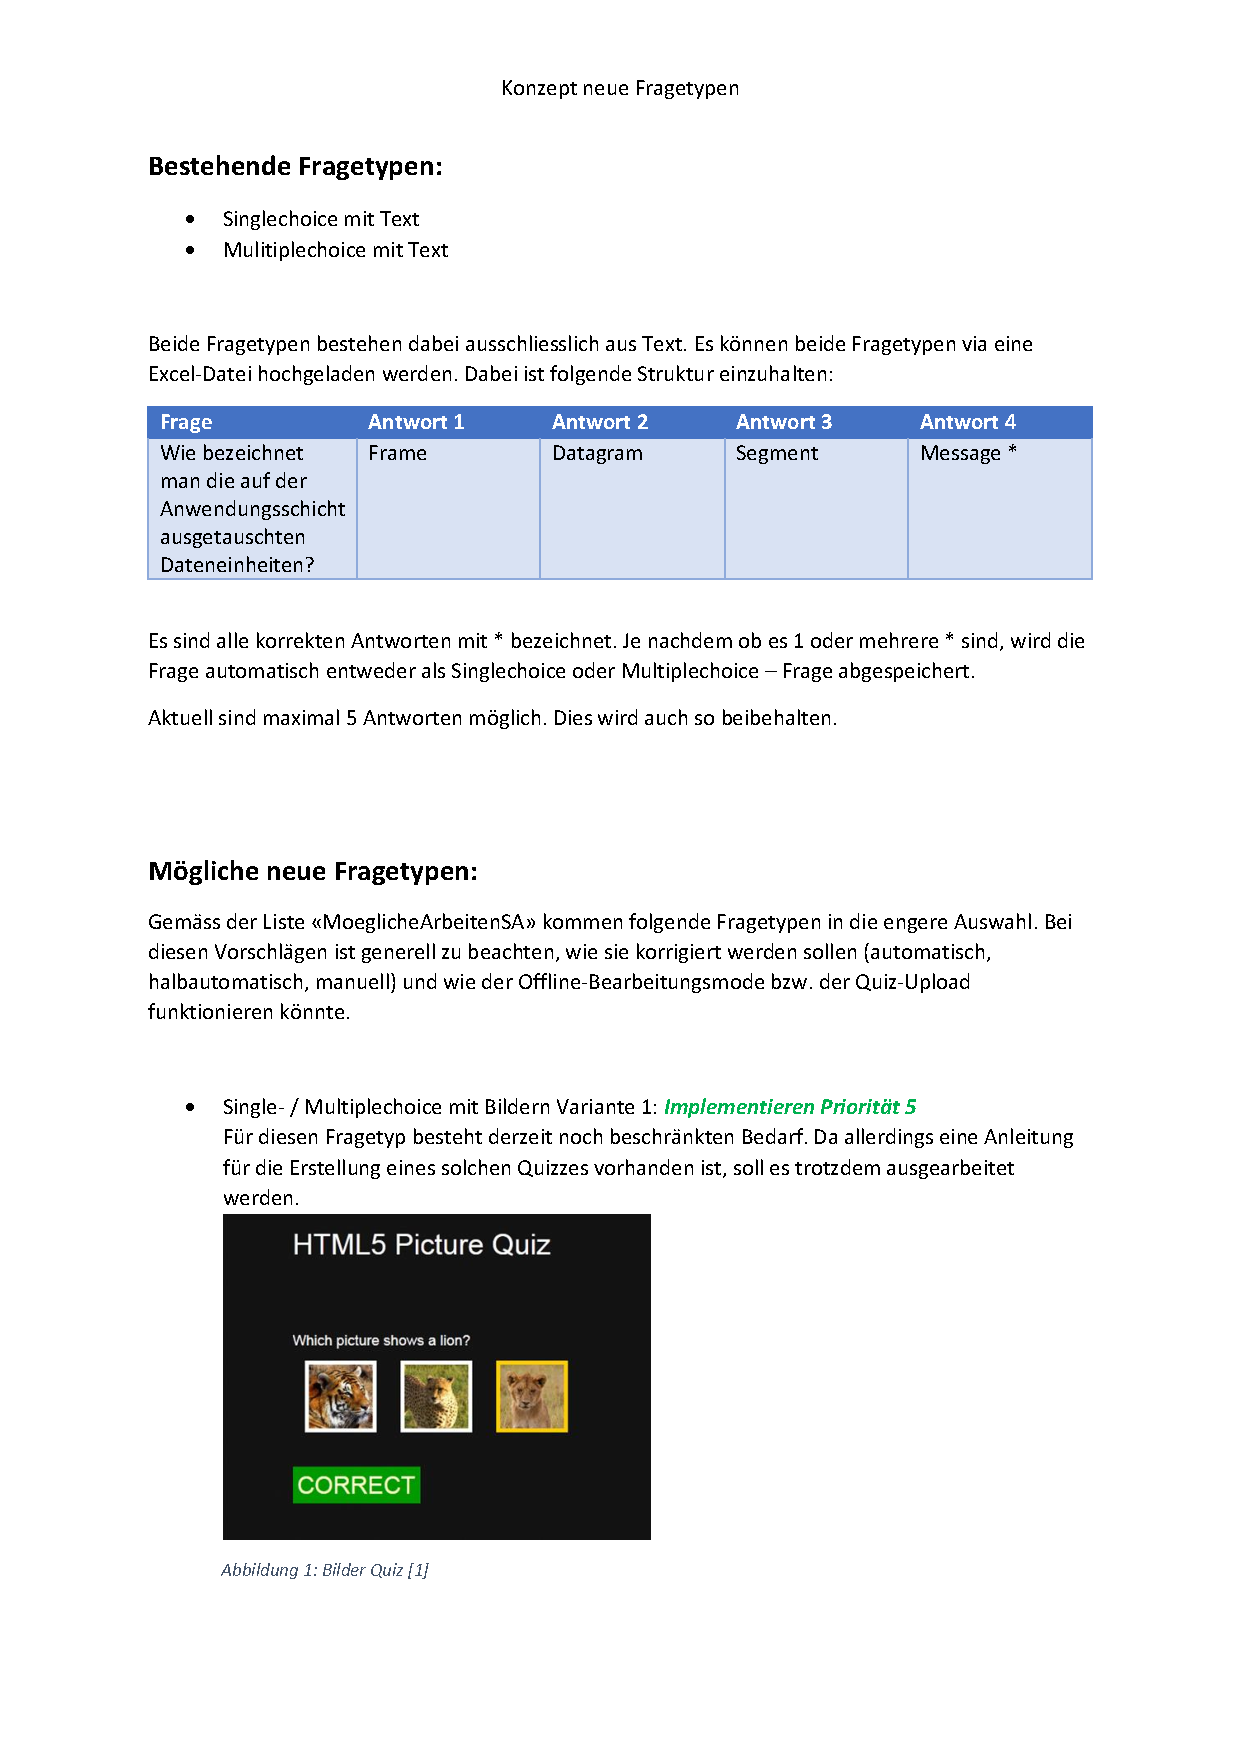
\includepdf[pages={1-13}, pagecommand={}]{PDFs/Neue_Fragetypen.pdf}
	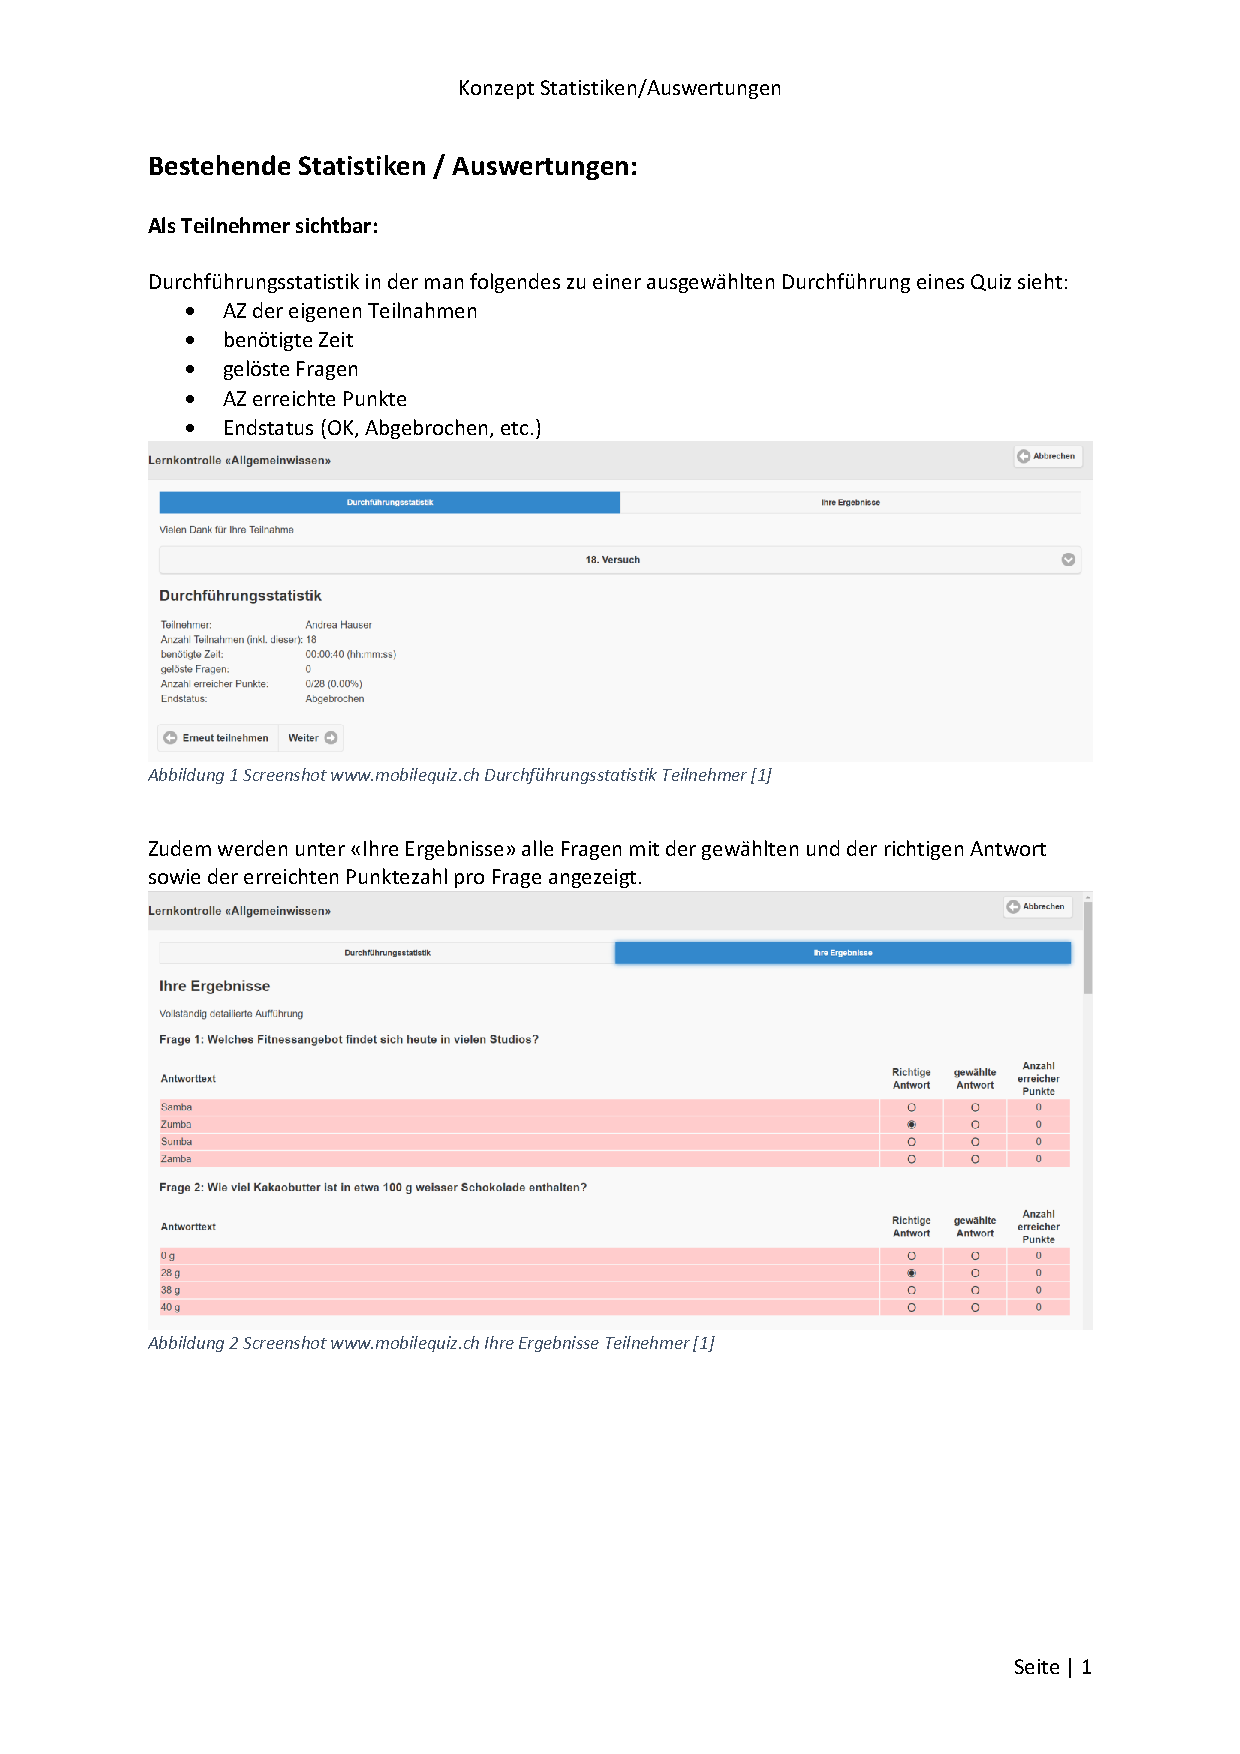
\includepdf[pages={1-12}, pagecommand={}]{PDFs/Statistiken_Auswertungen.pdf}
	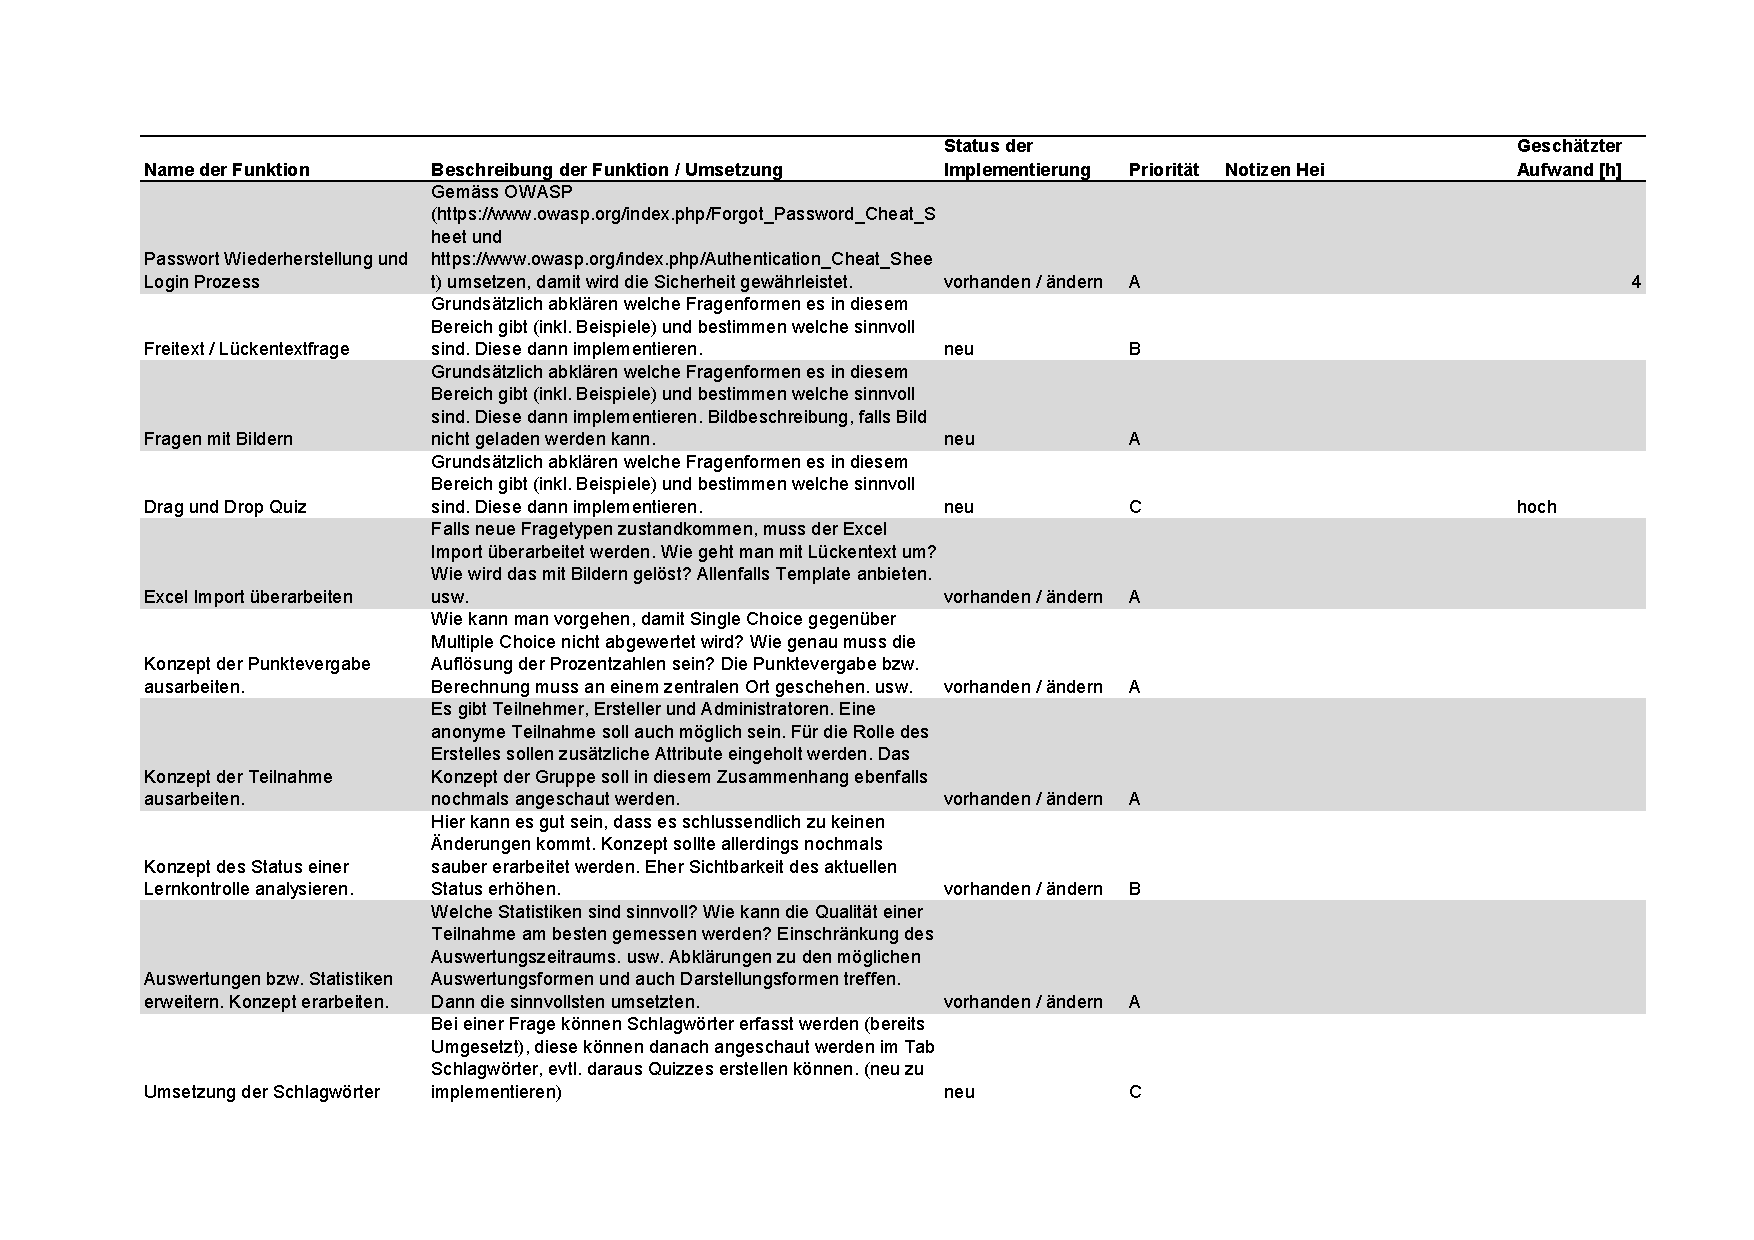
\includepdf[pages={1-3}, landscape=true, pagecommand={}]{PDFs/MoeglicheArbeitenSA.pdf}
	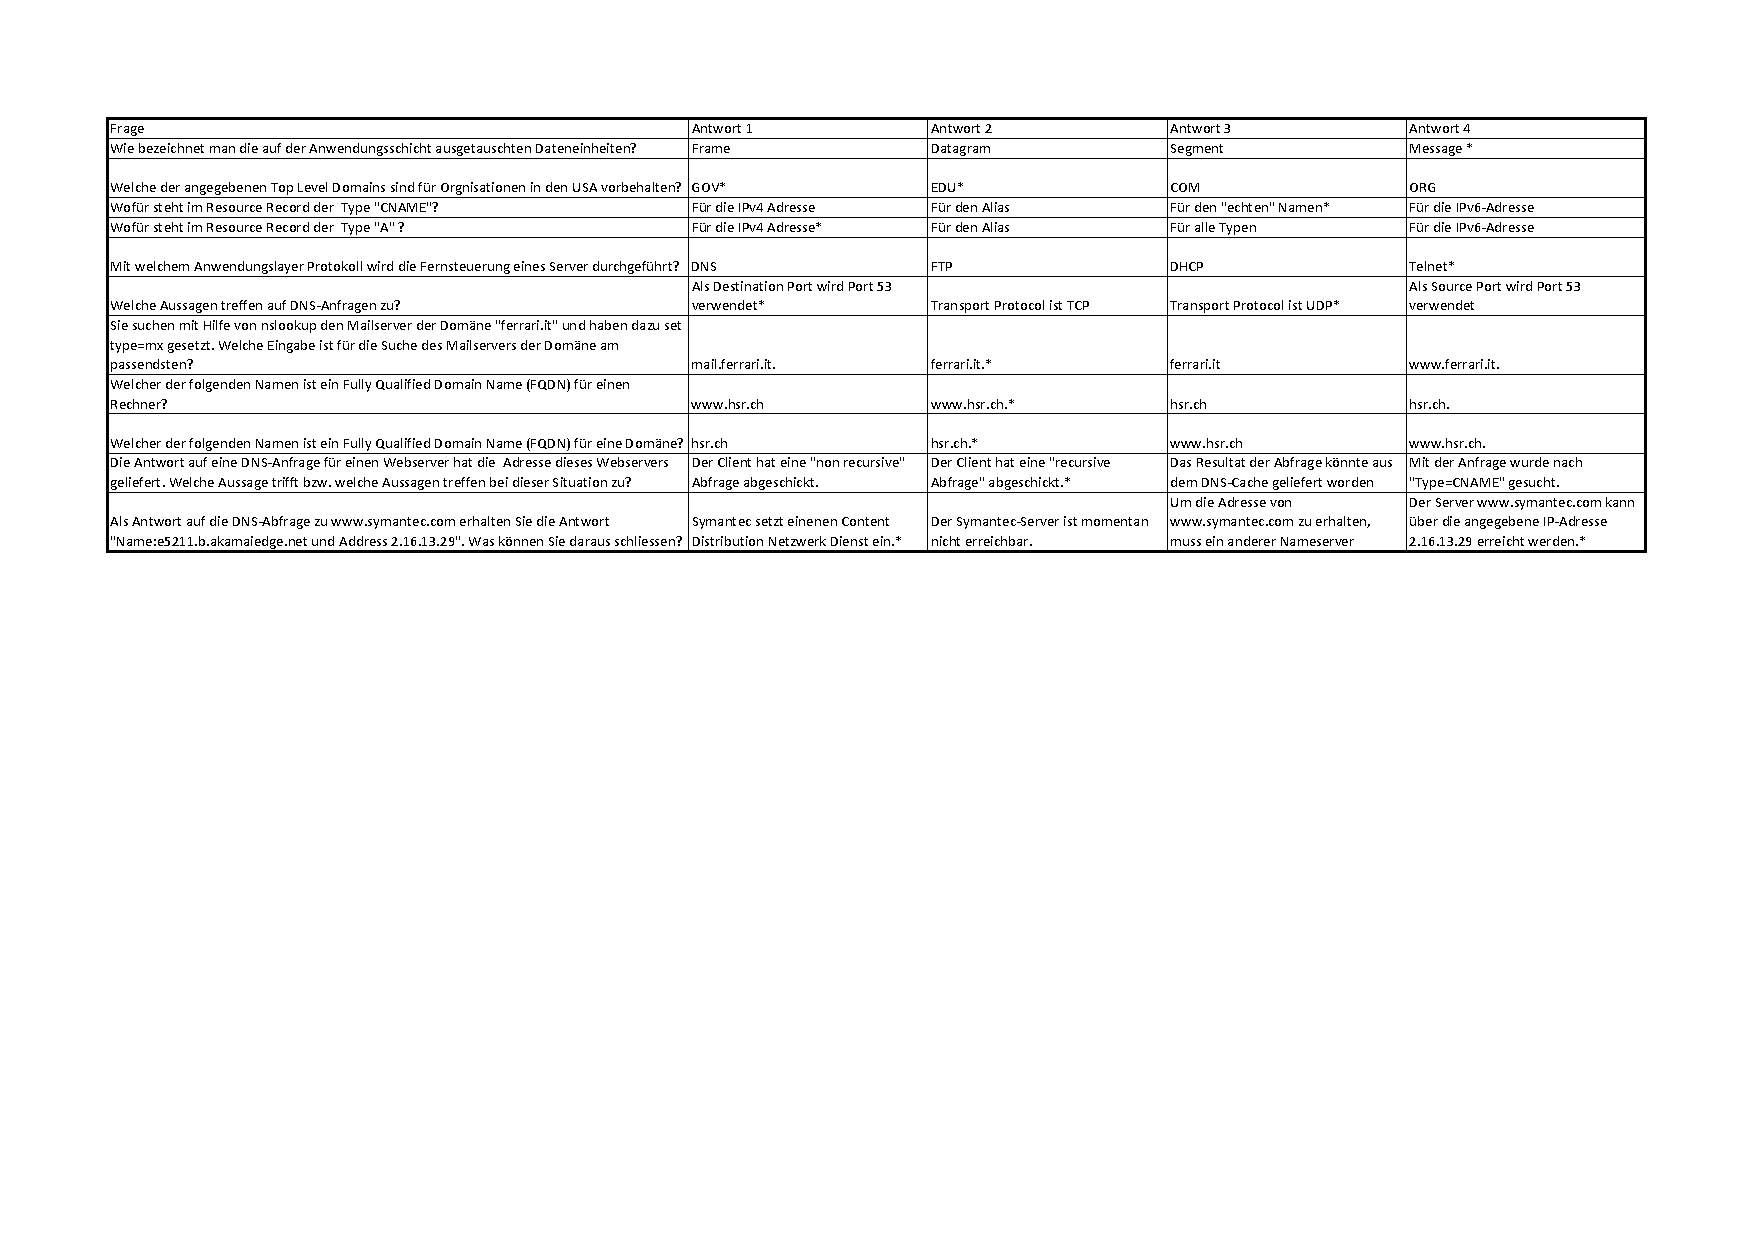
\includepdf[landscape=true, pagecommand={}]{PDFs/CSV_Template.pdf}
	\includepdf[landscape=true, pagecommand={}]{PDFs/socrativeQuizTemplate.pdf}
	\includepdf[landscape=true, pagecommand={}]{PDFs/Excel-Frage-Template.pdf}
	\includepdf[pages={1-3}, pagecommand={}]{PDFs/Recherchetipps_book-a-librarian.pdf}
	
	
	\chapter{Mockups}
	\label{chap:mockups}
	Alle nachfolgenden Mockups wurden mit dem Online-Mockup-Tool myBalsamiq erstellt. Die Lizenz wurde von der HSR zur Verfügung gestellt.
	
	Durch die nachträgliche Besprechung mit dem Betreuer wurden die nachfolgenden  Änderungen beschlossen, wodurch nicht mehr alle Mockups auf dem neusten Stand sind.
	\begin{itemize}
		\item Quiz-Informations-Seite\\
		Bereits umgesetzt:\\
		Auf dieser Seite wird der \glqq Start-Button\grqq nach rechts verschoben, links wird neu ein \glqq zur Übersicht\grqq - Button hinzugefügt. Zudem werden «Anzahl Fragen» und «Maximal mögliche Punktzahl» in der Reihenfolge geändert.\\
		Noch offen:\\
		Wenn der Start nicht mehr möglich ist, soll der Button ausgegraut werden.
		\item Durchführungsstatistik\\
		Noch offen:\\
		Das Datum der Durchführung soll immer angezeigt werden.
		\item Quiz-Erstellung\\
		Bereits umgesetzt:\\
		Statt \glqq Beschreibung\grqq soll \glqq Kommentar\grqq verwendet werden. Die Tabs im Quiz Erstellen sollen \glqq Allgemeine Informationen, Fragen und Durchführung\grqq heissen. Die Quiz Administration fällt weg. Das Hinzufügen von speziellen Berechtigungen wird in den Allgemeinen Informationen gemacht. Um die neuen Fragen zu erstellen wird das gleiche Konzept wie bei der Quiz Erstellung verwendet. Es wird dann vom Button \glqq Fragen erstellen\grqq auf die neue Seite \glqq Fragen erstellen\grqq weitergeleitet.
		
		\item Durchführungsoptionen\\
		Durchführungsoptionen sollen so nicht umgesetzt werden, stattdessen wird immer gleich die Einstellung in der Standardeinstellung angezeigt, wie dies bereits beim bestehenden Mobile Quiz der Fall ist. Rechts ist jeweils ein \glqq Zurücksetzen\grqq - Button, mit die jeweilige Einstellung auf den Standard-Wert zurückgesetzt werden kann.
		
	\end{itemize}
	
	\includepdf[pages={1-19}, landscape=true, pagecommand={}]{PDFs/MockupsVersion2.pdf}
	
	
	\chapter{Server-Anpassungen}
	%Alle Änderungen am Server, welche während der Entwicklung vorgenommen wurden
	
	\section{Änderungen am Server}
	\textbf{Wichtig:} 
	Für den Server-Upload müssen die folgenden zwei Dinge gegeben sein:
	\begin{itemize}
		\item Die PHP-Library 'GD' muss für die Bildverarbeitung installiert sein. Ob dies der Falls ist kann mittels PHPInfo() oder nachfolgendem Code festgestellt werden. \cite{zoopable.com} Sollte 'GD' nicht installiert sein, so ist unten ebenfalls der Installationsbefehl aufgeführt. \cite{askubuntu.com_php_extension}
	\end{itemize}
	\begin{lstlisting}
	<?php
	if (extension_loaded('gd') && function_exists('gd_info')) {
	echo "PHP GD library is installed on your web server";
	}
	else {
	echo "PHP GD library is NOT installed on your web server";
	}
	?>
	
	sudo apt-get install php5.6-gd
	\end{lstlisting}
	
	\begin{itemize}
		\item Die Childprozesse des Apache-Servers, welche die Anfragen beantworten, benötigen Schreibrechte auf den Upload-Ordner. Ob dies gegeben ist, kann mittels folgendem Befehl überprüft und geändert werden. \cite{askubuntu.com_permissions} 
	\end{itemize}
	\begin{lstlisting}
	ps -ef | grep apache | grep -v grep
	\end{lstlisting}
	
	\begin{lstlisting}
	root      5001     1  0 07:21 ?    00:00:00 /usr/sbin/apache2 -k start
	www-data  5021  5001  0 07:21 ?    00:00:00 /usr/sbin/apache2 -k start
	www-data  5022  5001  0 07:21 ?    00:00:00 /usr/sbin/apache2 -k start
	www-data  5023  5001  0 07:21 ?    00:00:00 /usr/sbin/apache2 -k start
	\end{lstlisting}
	
	Ist die Ausgabe wie oben ersichtlich, so werden die Anfragen von Prozessen der Benutzergruppe 'www-data' beantwortet. Die Schreibrechte an diese Gruppe können wie folgt vergeben werden:
	\begin{lstlisting}
	chgrp www-data /path/to/mydir
	chmod g+w /path/to/mydir
	\end{lstlisting}
	
	\includepdf[pages={1-4}, pagecommand={}]{PDFs/V2_Apache_PHP_MySQL-Docker.pdf}
	\includepdf[pages={1-3}, pagecommand={}]{PDFs/V3_Apache_PHP_MySQL-Ubuntu.pdf}
	\includepdf[pagecommand={}]{PDFs/Anleitung_Redmine_Datenbank_Backup.pdf}
	\includepdf[pagecommand={}]{PDFs/Aenderungen_Studenten_nach_Patrick_Eichler.pdf}
	
	\chapter{Projektmanagementplan}
	%Projektmanagementplan (kommentierter Arbeitsplan, Zeiterfassung: Durch den Einbezug des Arbeitsplans in den Bericht sollen die Studenten zu einer bewussten Arbeitsplanung animiert werden, sodass sie lernen den Arbeitsaufwand abzuschätzen und die Arbeit optimal zu organisieren.
	
	Da für die Umsetzung der neuen Features voraussichtlich mehr Zeit benötigt wird, wird eine weitere Construction-Phase angehängt und die erste Transition-Phase gestrichen.
	
	Bemerkung zur Präsentation:
	Am Anfang wäre eine Zeitachse mit den Meilensteinen noch gut gewesen, um eine Projekt-Übersicht zu geben. Diese Zeitachse hätte man dann als roter Faden verwenden können.
	
	% !TEX root = Projektdokumentation.tex

 \section{Kostenvoranschlag}
 Das Projekt läuft im Rahmen der Studienarbeit. Diese sieht einen Personenaufwand von 240 Stunden pro Person vor, was bei einer 2-Personen-Gruppe einen Aufwand von 480 Stunden macht. 
 Der Projektrahmen ist das Herbstsemester 2016, welches vom 19.09 - 23.12.2016 dauert und somit 14 Wochen umfasst. Es ist damit ein durchschnittlicher Wochenaufwand von 17 Stunden pro Person vorgesehen.
 
 
 \section{Zeitliche Planung}
 
 \subsection{Phasen / Iterationen}
 Das Projekt ist in die Phasen Inception, Elaboration, Construction und Transition aufgeteilt. Die Inception-Phase hat bereits in der Woche vor dem Semesterbeginn stattgefunden. Die restlichen Phasen sind, wie in der Grafik auf der nächsten Seite ersichtlich, über das Herbstsemesters 2017 verteilt.
 
 \includepdf[landscape=true]{Zeitplan_Spitzenbelastung.pdf}
 \todo{David Plan anpassen}
 
 \subsection{Meilensteine}
 
 %Die Meilensteine sollen konkret und messbar dargestellt werden.
 
 \begin{tabularx}{\linewidth}{|X|c|X|}
 	\hline
 	\textbf{Meilenstein} & \textbf{Datum} & \textbf{Beschreibung} \\
 	\hline
 	Finalisierte Aufgabenstellung & 09.10.2016 & Herr Heinzmann hat die zu erledigenden Arbeiten in einer Aufgabenstellung zusammengestellt und an die Studenten abgegeben. \\
 	\hline
 	End of Elaboration & 16.10.2016 & Die Umfeldanalyse ist abgeschlossen und es ist bekannt, welche Arbeiten im Rahmen der Studienarbeit angegangen werden. \\
 	\hline
 	Erster Teil des Berichts komplett & 30.10.2016 & Die Ergebnisse der Analyse-Phase sind vollständig niedergeschrieben, damit Herr Heinzmann diese gegenlesen kann. \\
 	\hline
 	Zwischenpräsentation & 13.11.2016 & Die bisher erarbeiteten Ergebnisse wurden Herrn Heinzmann als Vortrag präsentiert. \\
 	\hline
 	Erster Prototyp & 13.11.2016 & Die Code-Änderungen für eine verbesserte Usability wurden vollständig implementiert, damit in der Folgewoche die zweiten Usability-Tests durchgeführt werden können. \\
 	\hline
 	End of Construction & 11.12.2016 & Alle Änderungen am Code wurden implementiert, sodass dieser wieder auf den cnlab-Server übertragen werden kann. \\
 	\hline
 	Schlussabgabe & 23.12.2016 & Alle Dokumente wurden abgabekonform erstellt, die Dokumentation gebunden, der Code auf CD gebrannt und alles an Herrn Heinzmann abgegeben. \\
 	\hline
 \end{tabularx}
 
 
 
 \section{Zeiterfassung}
 Für alle Arbeiten werden in Redmine Arbeitspakete erfasst. Sofort nachdem ein Paket bearbeitet wurde, wird die Zeit darauf verbucht. Da alle Pakete einer Kategorie zugeordnet sind, kann am Ende des Projekts genau festgestellt werden, wie viel Zeit beispielsweise für alle Dokumentationen aufgewendet wurde.
 
 Die bereits erfassten Pakete sowie deren Fortschritt sind auf den folgenden Seiten abgebildet:
 
 \includepdf[landscape=true,pages={1-3}]{sa_mobilequiz-gantt_22-10-2016.pdf}
	
	\chapter{Risikomanagement}
	%Bezug nehmen auf das Excel.
	Eine Übersicht aller technischen Risiken befindet sich auf der folgenden Seite. Darin ist der aktuelle Zustand aller uns bekannten Risiken ersichtlich.
	
	\section{Umgang mit Risiken}
	Die Teammitglieder sind bereit, bei unerwarteten oder nicht vorhergesehenen Zwischenfällen das Arbeitspensum für die Studienarbeit zu erhöhen, um den fristgerechten Abschluss der Arbeit zu gewährleisten, solange es sich dabei nicht um einen Dauerzustand handelt. Zusätzlich wird bei der Schätzung der Aufwände immer darauf geachtet, für unerwartetes eine Reserve einzuplanen.
	Nach jeder Iteration werden die bestehenden Risiken neu evaluiert und falls nötig angepasst oder neue Risiken aufgenommen.
	
	\includepdf[landscape=true, pagecommand={}]{PDFs/TechnischeRisiken.pdf} 

	\chapter{Verwendete Werkzeuge}
	\label{chap:werkzeuge}
	% !TEX root = Projektdokumentation.tex

\section{Dokumentenverwaltung}

\begin{description}
	\item [OneDrive] ist ein Dienst von Microsoft, um Dateien auf einem zentralen Speicherort abzulegen. Auf diesen kann über das Internet zugegriffen werden. \cite{wikipedia_filehosting} \cite{wikipedia_oneDrive}
	\begin{itemize}
		\item Einsatzzweck: Dokumentenablage
		\item Version: 17.3
		\item Bezugsquelle: https://onedrive.live.com/about/de-de/download/
		\item Beachten: Benötigt kostenlose Registrierung auf https://onedrive.live.com/
	\end{itemize}
	
	
	\item [GitHub] ist ein Online Versionsverwaltungssystem für Software.
	\begin{itemize}
		\item Einsatzzweck: Versionskontrolle für Code und Latex-Projektdokumentation
		\item Version: unbekannt
		\item Webseite: https://github.com/
		\item Beachten: Benötigt kostenlose Registrierung auf https://github.com/join. Gratis Private-Repositories gibt es als Studenten mit der Registrierung auf https://education.github.com/pack
	\end{itemize}
	
	
	\item [GitHub Desktop] ist ein Programm für Windows und macOS, um GitHub-Repositories zu lokal synchronisieren und verwalten.
	\begin{itemize}
		\item Einsatzzweck: Synchronisation von Code und Latex-Projektdokumentation
		\item Version: 3.3.1.0
		\item Bezugsquelle: https://desktop.github.com/
	\end{itemize}
\end{description}



\newpage
\section{Server-Zugriff}

\begin{description}
	\item [FileZilla Client] ist ein Programm für Windows, macOS und Linux, um mittels FTP (File Transfer Protocol) Daten auf einen Server hoch- und herunterzuladen. \cite{wikipedia_filezilla}
	\begin{itemize}
		\item Einsatzzweck: Dateien auf HSR-Server hochladen
		\item Version: 3.22.1
		\item Bezugsquelle: http://filezilla.de/
	\end{itemize}
	
	
	\item [PuTTY] ist ein Programm für Windows und Linux, um Verbindungen mittels SSH (Secure Shell), Telnet oder über eine serielle Schnittstelle herzustellen. \cite{wikipedia_putty}
	\begin{itemize}
		\item Einsatzzweck: SSH-Verbindung zum HSR-Server, um Installationen oder Konfigurationen vorzunehmen.
		\item Version: 0.67
		\item Bezugsquelle: http://www.putty.org/
	\end{itemize}
\end{description}



\section{Projektverwaltung}

\begin{description}
	\item [Redmine] ist eine web-basierte Projektmanagement-Software.
	\begin{itemize}
		\item Einsatzzweck: Projektplanung, Ticketverwaltung und Zeiterfassung
		\item Version: 3.3.0.stable
		\item Bezugsquelle: Von Schule vorinstalliert.
	\end{itemize}
\end{description}


\newpage
\section{Dokumentation}

\begin{description}
	\item [Microsoft Office] ist ein Paket von Büro-Software für Windows, macOS, iOS, Android und Windows Phone. \cite{wikipedia_microsoft-office}
	\begin{itemize}
		\item Einsatzzweck: Dokumenten- und Tabellenerstellung, ausser Projektdokumentation
		\item Version: 1609
		\item Bezugsquelle: https://products.office.com/
		\item Beachten: Das Office-Paket kann als HSR-Student kostenlos heruntergeladen werden.
	\end{itemize}
	
	
	\item [TeXstudio] ist ein LaTex-Editor für Windows, macOS und Linux.
	\begin{itemize}
		\item Einsatzzweck: Erstellung von LaTex-Dokumenten, vor allem für Projektdokumentation
		\item Version: 2.11.0
		\item Bezugsquelle: http://www.texstudio.org/
		\item Beachten: Für die Erstellung von LaTex-Dokumenten benötigt es eine TeX-Distribution (siehe MiKTeX). Weiter ist ein Perl-Interpreter Voraussetzung, um ein Glossar zu erstellen.
	\end{itemize}
	
	
	\item [MiKTeX] ist eine TeX-Distribution für Windows. \cite{wikipedia_miktex}
	\begin{itemize}
		\item Einsatzzweck: Interpretation und Kompilation von LaTex-Dokumenten
		\item Version: 2.9
		\item Bezugsquelle: https://miktex.org/download
	\end{itemize}
	
	
	\item [ActivePerl] ist ein Perl-Interpreter für Windows.
	\begin{itemize}
		\item Einsatzzweck: Erstellung von LaTex-Glossaren
		\item Version: 5.24.0
		\item Bezugsquelle: http://www.activestate.com/activeperl
	\end{itemize}
	
	
	\item [Zotero] ist eine Quellenverwaltungs-Software für Windows, macOS und Linux.
	\begin{itemize}
		\item Einsatzzweck: Quellenverwaltung
		\item Version: 4.0.29.10
		\item Bezugsquelle: https://www.zotero.org/download/
		\item Beachten: Für das Speichern von neuen Quellen eignet sich das Browser-AddOn. Weiter können die Exporteinstellungen des Zotero-Standalone auf BibTeX eingestellt werden, was es ermöglicht, neue Quellen per Drag\&Drop einer .bib-Datei hinzuzufügen. So können neue Quellen schnell und einfach in LaTeX eingebunden werden.
	\end{itemize}
\end{description}



\section{Software-Entwicklung}

\begin{description}
	\item [PHP Eclipse] ist eine PHP-Entwicklungsumgebung für Windows, macOS und Linux.
	\begin{itemize}
		\item Einsatzzweck: PHP-Entwicklung
		\item Version: Neon.1 Release (4.6.1)
		\item Bezugsquelle: https://eclipse.org/pdt/
	\end{itemize}	
	
	
	\item [XAMPP Control Panel] ist eine PHP-Entwicklungsumgebung für Windows, macOS und Linux. Sie enthält Apache, MariaDB, PHP und Perl.
	\begin{itemize}
		\item Einsatzzweck: Lokale PHP-Entwicklung und Debugging. Über phpMyAdmin konnte die Datenbank leicht lokal installiert werden. Weiter ist der Apache-Server schnell eingerichtet. Da der Eclipse-Workspace im htdocs von Apache liegt, können Änderungen sofort nachvollzogen werden. Zudem ermöglicht die Kombination mit easy Xdebug (s. unten) ein einfaches Debugging mit Firefox und Eclipse.
		\item Version: 3.2.2
		\item Bezugsquelle: https://www.apachefriends.org/de/index.html
	\end{itemize}
	
	
	\item [easy Xdebug (with moveable icon)] ist ein Firefox AddOn, um einfaches Debugging mittels Eclipse zu ermöglichen.
	\begin{itemize}
		\item Einsatzzweck: Debugging mit Eclipse
		\item Version: 0.9.4
		\item Bezugsquelle: https://addons.mozilla.org/de/firefox/addon/easy-xdebug-with-moveable-
		\item Beachten: Es ist folgendermassen vorzugehen, um PHP mit Eclipse zu debuggen:
		\begin{enumerate}
			\item XAMPP Control Panel: Start von MySQL und Apache
			\item Start von Eclipse und Öffnen des Projekts
			\item Start von Firefox
			\item Firefox: Aktivierung des Toggle xdebug (roter Punkt sichtbar)
			\item Firefox: Navigation zu localhost/\textless Projektname in htdocs\textgreater
			\item Nun sollte Eclipse aufleuchten und fragen, ob in den Debug-Mode umgestellt werden soll.
		\end{enumerate}
	\end{itemize}
	
	
	\item [Selenium IDE] ist ein Firefox AddOn für Web-UI-Tests. Es ermöglicht das Aufnehmen, die Bearbeiten, das Debuggen und das Abspielen von Tests.
	\begin{itemize}
		\item Einsatzzweck: Erstellen und Abspielen von Web-UI-Tests
		\item Version: 2.9.1.1
		\item Bezugsquelle: https://addons.mozilla.org/de/firefox/addon/selenium-ide/
	\end{itemize}
\end{description}



\section{Continuous Integration}

\begin{description}
	\item [Travis] ist ein Online Continuous-Integration Service für GitHub-Projekte.
	\begin{itemize}
		\item Einsatzzweck: Builden und Unit-Testen von PHP-Code
		\item Version: unbekannt
		\item Webseite: https://travis-ci.org/ und https://travis-ci.com/
		\item Beachten: Als Student mit dem GitHub Student Developer Pack kann man unter https://travis-ci.com/ Private-Repositories kostenlos builden.
	\end{itemize}
	
	
	\item [Code Climate] ist ein Online Service, um die Code-Qualität und Test-Coverage zu messen.
	\begin{itemize}
		\item Einsatzzweck: Qualitätsmessung des PHP-Codes
		\item Version: 1.0
		\item Webseite: https://codeclimate.com/
		\item Beachten: Code Climate kann mit Travis verknüpft werden. Hat Travis alle Tests durchgeführt, so leitet er dann die Ergebnisse direkt weiter. Siehe dazu die Datei '.travis.yml'. Die Konfiguration für die Qualitäts-Tests von Code Climate sind in '.codeclimate.yml' festgelegt.
	\end{itemize}
\end{description}



\section{Usability}

\begin{description}
	\item [myBalsamiq] ist ein Online Service für die Erstellung von Mockups.
	\begin{itemize}
		\item Einsatzzweck: Erstellung von Mockups
		\item Version: Build \#release/4832 - 4832
		\item Webseite: https://www.mybalsamiq.com/
		\item Beachten: Als HSR-Student kann man dem Informatik-Studiengangleiter eine Anfrage schreiben, um kostenlos ein Projekt auf myBalsamiq erstellen zu können.
	\end{itemize}
\end{description}

	
	
	\chapter{Kontaktadressen}
	\label{LastPage}
	%Kontaktadressen von allen beteiligten Personen (Adressen der Studenten, über welche sie auch nach der Zeit an der HSR erreicht werden können, Industriepartner, Betreuer, weitere Personen)
	\begin{multicols}{2}
	\noindent \textbf{Studenten:}
	\\
	Andrea Hauser\\
	Waldheim 1\\
	8825 Hütten\\
	E-Mail: andrea.hauser@hotmail.ch\\
	\\
	David Windler\\
	Heid 320\\
	9502 Braunau\\
	\columnbreak
	E-Mail: david.windler@windowslive.com\\
	\textbf{Betreuer:}\\
	Prof. Dr. Peter Heinzmann (Dozent)\\
	E-Mail: peter.heinzmann@hsr.ch\\
	\\
	Patrick Eichler (Assistent)\\
	E-Mail: patrick.eichler@hsr.ch\\
	
	\end{multicols}
	
	

	
	
	
\end{document}